\documentclass{article}

  % packages
    % basic stuff for rendering math
    \usepackage[letterpaper, top=1in, bottom=1in, left=1in, right=1in]{geometry}
    \usepackage[utf8]{inputenc}
    \usepackage[english]{babel}
    \usepackage{amsmath} 
    \usepackage{amssymb}
    % \usepackage{amsthm}

    % extra math symbols and utilities
    \usepackage{mathtools}        % for extra stuff like \coloneqq
    \usepackage{mathrsfs}         % for extra stuff like \mathsrc{}
    \usepackage{centernot}        % for the centernot arrow 
    \usepackage{bm}               % for better boldsymbol/mathbf 
    \usepackage{enumitem}         % better control over enumerate, itemize
    \usepackage{hyperref}         % for hypertext linking
    \usepackage{fancyvrb}          % for better verbatim environments
    \usepackage{newverbs}         % for texttt{}
    \usepackage{xcolor}           % for colored text 
    \usepackage{listings}         % to include code
    \usepackage{lstautogobble}    % helper package for code
    \usepackage{parcolumns}       % for side by side columns for two column code
    

    % page layout
    \usepackage{fancyhdr}         % for headers and footers 
    \usepackage{lastpage}         % to include last page number in footer 
    \usepackage{parskip}          % for no indentation and space between paragraphs    
    \usepackage[T1]{fontenc}      % to include \textbackslash
    \usepackage{footnote}
    \usepackage{etoolbox}

    % for custom environments
    \usepackage{tcolorbox}        % for better colored boxes in custom environments
    \tcbuselibrary{breakable}     % to allow tcolorboxes to break across pages

    % figures
    \usepackage{pgfplots}
    \pgfplotsset{compat=1.18}
    \usepackage{float}            % for [H] figure placement
    \usepackage{tikz}
    \usepackage{tikz-cd}
    \usepackage{circuitikz}
    \usetikzlibrary{arrows}
    \usetikzlibrary{positioning}
    \usetikzlibrary{calc}
    \usepackage{graphicx}
    \usepackage{algorithmic}
    \usepackage{caption} 
    \usepackage{subcaption}
    \captionsetup{font=small}

    % for tabular stuff 
    \usepackage{dcolumn}

    \usepackage[nottoc]{tocbibind}
    \pdfsuppresswarningpagegroup=1
    \hfuzz=5.002pt                % ignore overfull hbox badness warnings below this limit

  % New and replaced operators
    \DeclareMathOperator*{\argmin}{\arg\!\min}
    \DeclareMathOperator*{\argmax}{\arg\!\max}
    \newcommand{\qed}{\hfill$\blacksquare$}     % I like QED squares to be black

  % Custom Environments
    \newtcolorbox[auto counter, number within=section]{exercise}[1][]
    {
      colframe = teal!25,
      colback  = teal!10,
      coltitle = teal!20!black,  
      breakable, 
      title = \textbf{Exercise \thetcbcounter ~(#1)}
    }
    \newtcolorbox[auto counter, number within=section]{solution}[1][]
    {
      colframe = violet!25,
      colback  = violet!10,
      coltitle = violet!20!black,  
      breakable, 
      title = \textbf{Solution \thetcbcounter}
    }
    \newtcolorbox[auto counter, number within=section]{theorem}[1][]
    {
      colframe = red!25,
      colback  = red!10,
      coltitle = red!20!black,  
      breakable, 
      title = \textbf{Theorem \thetcbcounter ~(#1)}
    } 
    \newtcolorbox[auto counter, number within=section]{proof}[1][]
    {
      colframe = orange!25,
      colback  = orange!10,
      coltitle = orange!20!black,  
      breakable, 
      title = \textbf{Proof. }
    } 
    \newtcolorbox[auto counter, number within=section]{definition}[1][]
    {
      colframe = yellow!25,
      colback  = yellow!10,
      coltitle = yellow!20!black,  
      breakable, 
      title = \textbf{Definition \thetcbcounter ~(#1)}
    } 
    \newtcolorbox[auto counter, number within=section]{example}[1][]
    {
      colframe = blue!25,
      colback  = blue!10,
      coltitle = blue!20!black,  
      breakable, 
      title = \textbf{Example \thetcbcounter ~(#1)}
    } 
    \newtcolorbox[auto counter, number within=section]{code}[1][]
    {
      colframe = green!25,
      colback  = green!10,
      coltitle = green!20!black,  
      breakable, 
      title = \textbf{Code \thetcbcounter ~(#1)}
    } 
    \newtcolorbox[auto counter, number within=section]{algo}[1][]
    {
      colframe = green!25,
      colback  = green!10,
      coltitle = green!20!black,  
      breakable, 
      title = \textbf{Algorithm \thetcbcounter ~(#1)}
    } 

    \definecolor{dkgreen}{rgb}{0,0.6,0}
    \definecolor{gray}{rgb}{0.5,0.5,0.5}
    \definecolor{mauve}{rgb}{0.58,0,0.82}
    \definecolor{darkblue}{rgb}{0,0,139}
    \definecolor{lightgray}{gray}{0.93}
    \renewcommand{\algorithmiccomment}[1]{\hfill$\triangleright$\textcolor{blue}{#1}}

    % default options for listings (for code)

    \lstdefinelanguage{arm}{
      keywords={add, adds, adc, adcs, sub, subs, sbc, sbcs, neg, negs, mul, smull, umull, smulh, umulh, madd, msub, sdiv, udiv, smaddl, smsubl, umaddl, umsubl, and, orr, eor, bic, orn, eon, mvn, lsl, lsr, asr, ror, cmp, cmn, tst, csel, csinc, csinv, csneg, ldr, ldrb, ldrh, ldrsb, ldrsh, ldrsw, str, strb, strh, ldp, stp, ldur, stur, ldar, stlr, ldxr, stxr, ldaxr, stlxr, b, bl, br, blr, ret, cbz, cbnz, tbz, tbnz, beq, bne, bcs, bhs, bcc, blo, bmi, bpl, bvs, bvc, bhi, bls, bge, blt, bgt, ble, bal, svc, hvc, smc, brk, hlt, isb, dsb, dmb, nop, yield, wfe, wfi, sev, sevl, fadd, fsub, fmul, fdiv, fabs, fneg, fsqrt, frintn, frintp, frintm, frintz, frinta, fcmp, fcmpe, fccmp, fccmpe, fcsel, fmov, fcvt, fcvtas, fcvtau, fcvtms, fcvtmu, fcvtns, fcvtnu, fcvtps, fcvtpu, fcvtzs, fcvtzu, scvtf, ucvtf, dup, ins, ext, zip1, zip2, uzp1, uzp2, trn1, trn2, rev16, rev32, rev64, cas, casa, casal, casl, swp, swpa, swpal, swpl, ldadd, ldclr, ldeor, ldset, ldsmax, ldsmin, ldumax, ldumin, mov, movk, movn, movz, adr, adrp, sxtb, sxth, sxtw, uxtb, uxth, uxtw, cls, clz, rbit, rev, sbfm, ubfm, bfm, extr, hint, prfm, prfum,
      },
      keywordstyle=\color{blue}\bfseries,
      comment=[l]{//},
      commentstyle=\color{green!60!black}\itshape,
      string=[b]",
      stringstyle=\color{red},
      basicstyle=\ttfamily\small,
      showstringspaces=false,
      breaklines=true,
      frame=single,
      numbers=left,
      numberstyle=\tiny\color{gray}
    }
    \lstdefinelanguage{assembly}{
      keywords={.globl, .local, .extern, .weak, .byte, .word, .quad, .asciz, .ascii, .space, .fill, .align, .p2align, .balign, .text, .data, .bss, .section, .ifdef, .else, .endif, .macro, .endm, mov, stp, bl, ret},
      keywordstyle=\color{blue}\bfseries,
      comment=[l]{//},
      commentstyle=\color{green!60!black}\itshape,
      string=[b]",
      stringstyle=\color{red},
      basicstyle=\ttfamily\small,
      showstringspaces=false,
      breaklines=true,
      frame=single,
      numbers=left,
      numberstyle=\tiny\color{gray}
    }

    \lstset{
      autogobble,
      frame=ltbr,
      language=assembly,
      aboveskip=3mm,
      belowskip=3mm,
      showstringspaces=false,
      columns=fullflexible,
      keepspaces=true,
      basicstyle={\small\ttfamily},
      numbers=left,
      firstnumber=1,                        % start line number at 1
      numberstyle=\tiny\color{gray},
      keywordstyle=\color{blue},
      commentstyle=\color{dkgreen},
      stringstyle=\color{mauve},
      backgroundcolor=\color{lightgray}, 
      breaklines=true,                      % break lines
      breakatwhitespace=true,
      tabsize=3, 
      xleftmargin=2em, 
      framexleftmargin=1.5em, 
      stepnumber=1
    }

  % Page style
    \pagestyle{fancy}
    \fancyhead[L]{Assembly}
    \fancyhead[C]{Muchang Bahng}
    \fancyhead[R]{Fall 2024} 
    \fancyfoot[C]{\thepage / \pageref{LastPage}}
    \renewcommand{\footrulewidth}{0.4pt}          % the footer line should be 0.4pt wide
    \renewcommand{\thispagestyle}[1]{}  % needed to include headers in title page
\begin{document}

\title{Assembly}
\author{Muchang Bahng}
\date{Fall 2024}

\maketitle
\tableofcontents
\pagebreak

This covers computability theory, complexity theory, and automata theory. 
Alphabet. Boolean logic


\section{ARM Data Movement} 

  At this point (assuming you are going through my computer science notes in order), we have encountered our first lexical computer language. We aren't just describing things with psuedocode like we did with architecture, and we aren't relying on hardware-like systems like circuits or Conway's game of life here. This extra level of abstraction is nice to work with, but in order to fully appreciate it, we must know how to convert assembly into machine code. As we have seen, this is done in two steps. 
  \begin{enumerate}
    \item \textit{Assemblers} convert them into object files. 
    \item \textit{Linkers} use a relocation table to convert them into executables, written in machine code. 
  \end{enumerate} 
  This is essentially a translation from one language into another, and to do this, we might want to have some organization in our code. Therefore, we divide \texttt{.s} files into \textit{sections}. Furthermore, we might want to include instructions that tell the assembler---not the CPU---how to process your code, analogous to preprocessing text or tuning parameters for translation. 

  Both sections and directives have a period \texttt{.} at the front of their name, so you must tell them apart by context. 

  \begin{definition}[Section]
    In order for assemblers and linkers to interpret your programs, we must organize them into \textbf{sections}. Each section---specified by the distinctive \texttt{.} at the front of its name---specifies the following non-exhaustive list of properties. 
    \begin{enumerate}
      \item The read/write/executable permissions. 
      \item How data is initialized. 
    \end{enumerate}
  \end{definition} 

  \begin{example}[Must-Know Sections]
    The main sections you should be familiar with are 
    \begin{enumerate}
      \item \texttt{.text} (read+execute). This is where you write your code. 
      \item \texttt{.data} (read+write). This is where you store data and memory. 
      \item \texttt{.rodata} (read). Stores constant data that should not be modified during program execution. 
      \item \texttt{.bss} (read+write). Zero-initialized and stores uninitialized variables. 
    \end{enumerate}
  \end{example} 

  You can also create your own sections. 

\subsection{Loading}

  The first thing you should know about are registers. Here are the register conventions for ARM64. 

  \begin{definition}[ARM64 Registers]
    A 64-bit program on an ARM processor has access to 31-general purpose registers, a program counter, and a stack pointer (aka a combination zero register). 
    \begin{enumerate}
      \item \texttt{X0} - \texttt{X30}. These 31 registers are general purpose. You can use them for anything you want, though there are some standards. 
      \item \texttt{SP, XZR}. The link register. If you call a function, this register will be used to hold the return address. 
      \item \texttt{PC}. Program counter. The memory address of the currently executing instruction. 
    \end{enumerate}
    All the X registers can be operated on as 32-bit registers by referring to them as W0–W30 and WZR. When we do this, the instruction will use the lower 32 bits of the register and set the upper 32 bits to zero. Using 32 bits saves memory, since you only use 4 bytes rather than 8 bytes for each quantity saved. 
    Some Apple specific things: 
    \begin{enumerate}
      \item Apple reserves X18 for its own use. Do not use this register. 
      \item The frame pointer register (\texttt{FP}, \texttt{X29}) must always address a valid frame record. This is for backtraces. 
    \end{enumerate}
  \end{definition}

  \begin{definition}[Data Movement Operations]
    \begin{lstlisting}[language=arm]
      # Basic move operations
      mov x0, x1            // Move register to register
      mov x0, #42           // Move immediate to register
      
      # Move with zero/not/keep
      movz x0, #0x1234      // Move immediate, zero other bits
      movn x0, #0x1234      // Move NOT of immediate
      
      # Conditional moves (covered in logical section)
      csel x0, x1, x2, eq   // Conditional select
      csinc x0, x1, x2, ne  // Conditional select and increment
      
      # Register to register with operations
      sxtb x0, w1           // Sign extend byte to 64-bit
      sxth x0, w1           // Sign extend halfword to 64-bit
      sxtw x0, w1           // Sign extend word to 64-bit
      uxtb w0, w1           // Zero extend byte to 32-bit
      uxth w0, w1           // Zero extend halfword to 32-bit
    \end{lstlisting}
  \end{definition} 

  \begin{definition}[Exit Codes]
    \textbf{Exit codes} are values that represent the status of a program upon termination. It is usually the number residing in \texttt{x0} and can take in value between $0$ and $255$, inclusive. Any other numbers will be truncated to its 8 LSBs. 
  \end{definition}

  \begin{definition}[Basic Load Operations]
    \begin{lstlisting}[language=arm]
      ldr x0, [x1]          // Load 64-bit from [x1]
      ldr w0, [x1]          // Load 32-bit from [x1]
      ldrh w0, [x1]         // Load 16-bit halfword (zero extend)
      ldrb w0, [x1]         // Load 8-bit byte (zero extend)
      
      # Sign-extending loads
      ldrsw x0, [x1]        // Load 32-bit, sign extend to 64-bit
      ldrsh x0, [x1]        // Load 16-bit, sign extend to 64-bit
      ldrsh w0, [x1]        // Load 16-bit, sign extend to 32-bit
      ldrsb x0, [x1]        // Load 8-bit, sign extend to 64-bit
      ldrsb w0, [x1]        // Load 8-bit, sign extend to 32-bit
    \end{lstlisting}
  \end{definition}

  \begin{definition}[Basic Store Operations]
    \begin{lstlisting}[language=arm]
      str x0, [x1]          // Store 64-bit to [x1]
      str w0, [x1]          // Store 32-bit to [x1]
      strh w0, [x1]         // Store 16-bit halfword to [x1]
      strb w0, [x1]         // Store 8-bit byte to [x1]
    \end{lstlisting}
  \end{definition}

  \begin{definition}[Addressing Modes]
    \begin{lstlisting}[language=arm]
      # Immediate offset
      ldr x0, [x1, #8]      // Load from [x1 + 8]
      str x0, [x1, #16]     // Store to [x1 + 16]
      
      # Register offset
      ldr x0, [x1, x2]      // Load from [x1 + x2]
      ldr x0, [x1, x2, lsl #3]  // Load from [x1 + (x2 << 3)]
      
      # Pre-indexed (update base register before)
      ldr x0, [x1, #8]!     // x1 = x1 + 8, then load from [x1]
      str x0, [x1, #-16]!   // x1 = x1 - 16, then store to [x1]
      
      # Post-indexed (update base register after)
      ldr x0, [x1], #8      // Load from [x1], then x1 = x1 + 8
      str x0, [x1], #16     // Store to [x1], then x1 = x1 + 16
    \end{lstlisting}
  \end{definition}

  \begin{definition}[Pair Load/Store Operations]
    \begin{lstlisting}[language=arm]
      # Load/store register pairs
      ldp x0, x1, [x2]      // Load pair: x0=[x2], x1=[x2+8]
      stp x0, x1, [x2]      // Store pair: [x2]=x0, [x2+8]=x1
      
      # With immediate offset
      ldp x0, x1, [x2, #16] // Load pair from [x2+16], [x2+24]
      stp x0, x1, [x2, #32] // Store pair to [x2+32], [x2+40]
      
      # Pre/post-indexed pairs
      ldp x0, x1, [x2, #16]!    // x2+=16, then load pair
      stp x0, x1, [x2], #16     // Store pair, then x2+=16
      
      # Mixed register sizes
      ldp w0, w1, [x2]      // Load 32-bit pair
      stp w0, w1, [x2]      // Store 32-bit pair
    \end{lstlisting}
  \end{definition}

  \begin{definition}[Atomic and Exclusive Operations]
    \begin{lstlisting}[language=arm]
      # Load/store exclusive
      ldxr x0, [x1]         // Load exclusive 64-bit
      stxr w2, x0, [x1]     // Store exclusive 64-bit (w2 = status)
      ldxrh w0, [x1]        // Load exclusive 16-bit
      stxrh w2, w0, [x1]    // Store exclusive 16-bit
      ldxrb w0, [x1]        // Load exclusive 8-bit
      stxrb w2, w0, [x1]    // Store exclusive 8-bit
      
      # Clear exclusive monitor
      clrex                 // Clear exclusive access monitor
      
      # Load/store exclusive pairs
      ldxp x0, x1, [x2]     // Load exclusive pair
      stxp w3, x0, x1, [x2] // Store exclusive pair (w3 = status)
    \end{lstlisting}
  \end{definition}

  \begin{definition}[PC-Relative Addressing]
    \begin{lstlisting}[language=arm]
      # Address generation
      adr x0, label         // Load address of label (PC + offset)
      adrp x0, label        // Load page address of label
      
      # PC-relative loads
      ldr x0, =value        // Load literal (assembler places in literal pool)
      ldr x0, label         // Load from label address
      
      # Combined page + offset addressing
      adrp x0, symbol@PAGE
      add x0, x0, symbol@PAGEOFF
      ldr x1, [x0]          // Load from symbol
    \end{lstlisting}
  \end{definition}

  \begin{definition}[Advanced Load/Store]
    \begin{lstlisting}[language=arm]
      # Load with acquire, store with release (memory ordering)
      ldar x0, [x1]         # Load acquire
      stlr x0, [x1]         # Store release
      ldarb w0, [x1]        # Load acquire byte
      stlrb w0, [x1]        # Store release byte
      ldarh w0, [x1]        # Load acquire halfword
      stlrh w0, [x1]        # Store release halfword
      
      # Prefetch operations
      prfm pldl1keep, [x0]  # Prefetch for load, L1 cache, keep
      prfm pstl1strm, [x0, #64]  # Prefetch for store, L1, streaming
      
      # Non-temporal loads/stores
      ldnp x0, x1, [x2]     # Load pair non-temporal
      stnp x0, x1, [x2]     # Store pair non-temporal
    \end{lstlisting}
  \end{definition}

\subsection{Arithmetic} 

  \begin{definition}[Addition]
    \begin{lstlisting}[language=arm]
      add x0, x1, x2      # x0 = x1 + x2 (64-bit)
      add w0, w1, w2      # w0 = w1 + w2 (32-bit)
      add x0, x1, #42     # x0 = x1 + 42 (immediate)
      adds x0, x1, x2     # Add and set flags
      adc x0, x1, x2      # Add with carry
      adcs x0, x1, x2     # Add with carry and set flags
    \end{lstlisting}
  \end{definition}

  \begin{definition}[Subtraction]
    \begin{lstlisting}[language=arm]
      sub x0, x1, x2      # x0 = x1 - x2
      sub w0, w1, w2      # 32-bit subtract
      sub x0, x1, #42     # x0 = x1 - 42
      subs x0, x1, x2     # Subtract and set flags
      sbc x0, x1, x2      # Subtract with carry
      sbcs x0, x1, x2     # Subtract with carry and set flags
      neg x0, x1          # x0 = -x1 (negate)
      negs x0, x1         # Negate and set flags
    \end{lstlisting}
  \end{definition}

  \begin{definition}[Multiplication]
    \begin{lstlisting}[language=arm]
      mul x0, x1, x2      # x0 = x1 * x2 (low 64 bits)
      smull x0, w1, w2    # Signed multiply 32 to 64 bit
      umull x0, w1, w2    # Unsigned multiply 32 to 64 bit
      smulh x0, x1, x2    # Signed multiply high (upper 64 bits)
      umulh x0, x1, x2    # Unsigned multiply high
      madd x0, x1, x2, x3 # x0 = x3 + (x1 * x2) (multiply-add)
      msub x0, x1, x2, x3 # x0 = x3 - (x1 * x2) (multiply-subtract)
    \end{lstlisting}
  \end{definition}

  \begin{definition}[Division]
    \begin{lstlisting}[language=arm]
      sdiv x0, x1, x2     # x0 = x1 / x2 (signed)
      udiv x0, x1, x2     # x0 = x1 / x2 (unsigned)
    \end{lstlisting}
  \end{definition}

  \begin{definition}[Multiply-Accumulate]
    \begin{lstlisting}[language=arm]
      madd x0, x1, x2, x3   # x0 = x3 + (x1 * x2)
      msub x0, x1, x2, x3   # x0 = x3 - (x1 * x2)
      smaddl x0, w1, w2, x3 # x0 = x3 + (w1 * w2) signed 32 to 64
      smsubl x0, w1, w2, x3 # x0 = x3 - (w1 * w2) signed 32 to 64
      umaddl x0, w1, w2, x3 # x0 = x3 + (w1 * w2) unsigned 32 to 64
      umsubl x0, w1, w2, x3 # x0 = x3 - (w1 * w2) unsigned 32 to 64
    \end{lstlisting}
  \end{definition}

  \begin{definition}[Bitwise Operations]
    \begin{lstlisting}[language=arm]
      and x0, x1, x2      # Bitwise AND
      orr x0, x1, x2      # Bitwise OR
      eor x0, x1, x2      # Bitwise XOR (exclusive OR)
      bic x0, x1, x2      # Bit clear (x0 = x1 & ~x2)
      orn x0, x1, x2      # OR NOT (x0 = x1 | ~x2)
      eon x0, x1, x2      # XOR NOT (x0 = x1 ^ ~x2)
      mvn x0, x1          # Move NOT (x0 = ~x1)
    \end{lstlisting}
  \end{definition}

  \begin{definition}[Shift Operations]
    \begin{lstlisting}[language=arm]
      lsl x0, x1, #5      # Logical shift left by 5
      lsr x0, x1, #3      # Logical shift right by 3
      asr x0, x1, #2      # Arithmetic shift right by 2
      ror x0, x1, #4      # Rotate right by 4
    \end{lstlisting}
  \end{definition}

  \begin{definition}[Combined Operations]
    \begin{lstlisting}[language=arm]
      # Add with shifted register
      add x0, x1, x2, lsl #3    # x0 = x1 + (x2 << 3)
      sub x0, x1, x2, asr #2    # x0 = x1 - (x2 >> 2)
      
      # Bitwise with shifted register  
      and x0, x1, x2, ror #4    # x0 = x1 & (x2 rotated right 4)
      orr x0, x1, x2, lsl #1    # x0 = x1 | (x2 << 1)
    \end{lstlisting}
  \end{definition}

  \begin{definition}[Comparison Operations]
    \begin{lstlisting}[language=arm]
      cmp x1, x2          # Compare (sets flags, x1 - x2)
      cmn x1, x2          # Compare negative (sets flags, x1 + x2)
      tst x1, x2          # Test (sets flags, x1 & x2)
    \end{lstlisting}
  \end{definition}

  \begin{definition}[Conditional Operations]
    \begin{lstlisting}[language=arm]
      csel x0, x1, x2, eq    # x0 = (condition) ? x1 : x2
      csinc x0, x1, x2, ne   # x0 = (condition) ? x1 : x2+1
      csinv x0, x1, x2, gt   # x0 = (condition) ? x1 : ~x2
      csneg x0, x1, x2, lt   # x0 = (condition) ? x1 : -x2
    \end{lstlisting}
  \end{definition}

  \begin{definition}[Absolute Value and Min/Max]
    \begin{lstlisting}[language=arm]
      # Using conditional select for abs(x1)
      cmp x1, #0
      csneg x0, x1, x1, ge    # x0 = (x1 >= 0) ? x1 : -x1
      
      # Min/max using conditional select
      cmp x1, x2
      csel x0, x1, x2, lt     # x0 = min(x1, x2)
      csel x0, x1, x2, gt     # x0 = max(x1, x2)
    \end{lstlisting}
  \end{definition}

  \begin{definition}[Increment/Decrement]
    \begin{lstlisting}[language=arm]
      add x0, x0, #1      # Increment by 1
      sub x0, x0, #1      # Decrement by 1
      adds x0, x0, #1     # Increment and set flags
      subs x0, x0, #1     # Decrement and set flags
    \end{lstlisting}
  \end{definition}

  \begin{definition}[Modulo Operation]
    \begin{lstlisting}[language=arm]
      # x0 = x1 % x2 (signed) - No direct instruction
      sdiv x3, x1, x2     # x3 = x1 / x2
      msub x0, x3, x2, x1 # x0 = x1 - (x3 * x2)
    \end{lstlisting}
  \end{definition}

  \begin{definition}[Power of 2 Operations]
    \begin{lstlisting}[language=arm]
      # Multiply by power of 2
      lsl x0, x1, #3      # x0 = x1 * 8 (2^3)
      
      # Divide by power of 2
      lsr x0, x1, #2      # x0 = x1 / 4 (unsigned)
      asr x0, x1, #2      # x0 = x1 / 4 (signed)
    \end{lstlisting}
  \end{definition}

\subsection{Logical Operations}

  \begin{definition}[Bit Field Operations]
    \begin{lstlisting}[language=arm]
      sbfx x0, x1, #5, #8   # Signed bit field extract
      ubfx x0, x1, #5, #8   # Unsigned bit field extract  
      sbfiz x0, x1, #5, #8  # Signed bit field insert zeros
      ubfiz x0, x1, #5, #8  # Unsigned bit field insert zeros
      bfi x0, x1, #5, #8    # Bit field insert
      bfxil x0, x1, #5, #8  # Bit field extract and insert low
    \end{lstlisting}
  \end{definition}

  \begin{definition}[Bit Manipulation]
    \begin{lstlisting}[language=arm]
      rbit x0, x1           # Reverse bits
      rev x0, x1            # Reverse bytes (64-bit)
      rev32 x0, x1          # Reverse bytes in 32-bit words
      rev16 x0, x1          # Reverse bytes in 16-bit halfwords
      clz x0, x1            # Count leading zeros
      cls x0, x1            # Count leading sign bits
    \end{lstlisting}
  \end{definition}

  \begin{definition}[Advanced Logical Operations]
    \begin{lstlisting}[language=arm]
      # Bitwise operations with immediates
      and x0, x1, #0xFF00   # AND with immediate mask
      orr x0, x1, #0x0F0F   # OR with immediate mask
      eor x0, x1, #0xAAAA   # XOR with immediate mask
      
      # Test and branch on bit
      tbz x1, #5, label     # Test bit zero and branch
      tbnz x1, #5, label    # Test bit non-zero and branch
    \end{lstlisting}
  \end{definition}

  \begin{definition}[Conditional Logic]
    \begin{lstlisting}[language=arm]
      ccmp x1, x2, #0, eq   # Conditional compare
      ccmn x1, x2, #0, ne   # Conditional compare negative
      cset x0, eq           # Conditional set (x0 = condition ? 1 : 0)
      csetm x0, ne          # Conditional set mask (x0 = condition ? -1 : 0)
      cinc x0, x1, gt       # Conditional increment
      cinv x0, x1, lt       # Conditional invert
      cneg x0, x1, ge       # Conditional negate
    \end{lstlisting}
  \end{definition}

  \begin{definition}[Logical Shift Operations]
    \begin{lstlisting}[language=arm]
      # Standalone shift operations
      lsl x0, x1, x2        # Logical shift left by register
      lsr x0, x1, x2        # Logical shift right by register
      asr x0, x1, x2        # Arithmetic shift right by register
      ror x0, x1, x2        # Rotate right by register
      
      # Shift with immediate
      lsl x0, x1, #5        # Logical shift left by immediate
      lsr x0, x1, #3        # Logical shift right by immediate
      asr x0, x1, #2        # Arithmetic shift right by immediate
      ror x0, x1, #4        # Rotate right by immediate
    \end{lstlisting}
  \end{definition}

  \begin{definition}[Pattern Operations]
    \begin{lstlisting}[language=arm]
      # Extract and duplicate patterns
      extr x0, x1, x2, #8   # Extract from register pair
      dup v0.8b, w1         # Duplicate scalar to vector
      
      # Bit pattern generation
      movz x0, #0x1234      # Move with zero (clear other bits)
      movn x0, #0x1234      # Move with NOT (invert pattern)
      movk x0, #0x5678, lsl #16  # Move and keep (insert pattern)
    \end{lstlisting}
  \end{definition}

\subsection{Assembling and Disassembling} 

  \begin{definition}[Instruction Syntax]
    Every ARM instruction---regardless of whether we're in 32-bit or 64-bit ARM---can be fit into 32 bits of memory. The fixed-length variable of this is good for speed.   
    
    \begin{figure}[H]
      \centering 
      \begin{tabular}{|c|c|c|c|c|c|c|c|c|c|}
      \hline
      \textbf{31} & \textbf{30} & \textbf{29} & \textbf{28-24} & \textbf{23-22} & \textbf{21} & \textbf{20-16} & \textbf{15-10} & \textbf{9-5} & \textbf{4-0} \\
      \hline
      Bits & Opcode & Set Condition Code & Opcode & Shift & 0 & Rm & Imm & Rn & Rd \\
      \hline
      \end{tabular}
      \caption{Instruction encoding format.} 
    \end{figure}

    \begin{enumerate}
      \item \textit{Bits}. If this bit is $0$, then any registers are interpreted as the 32-bit \texttt{W} version. If $1$, then they are the full 64-bit version of the register.\footnote{You cannot mix W and Z bits in the same instruction!}

      \item \textit{Opcode}. which instruction are we performing, e.g. \texttt{ADD} or \texttt{MUL}. 

      \item \textit{Shift}. These two bits specify shifting operations that could be applied to the data. 

      \item \textit{Set Condition Code}. A single bit indicating if this instruction should update any condition flags. If we don't want the result of this instruction to affect following branch instructions, we set it to $0$. 

      \item \textit{Rm, Rn}. Operand registers to use as input. 
        
      \item \textit{Rd}. Destination register, i.e. where to put the result of whatever this instruction does. 

      \item \textit{Imm6}. An immediate operand which is usually a small bit of data that you can specify directly in the instruction. So, if you want to add 1 to a register, you could have this as 1, rather than putting 1 in another register and adding the two registers. These are usually the bits left over after everything else is specified.
    \end{enumerate}
  \end{definition}

  A \textbf{dump} refers to a representation of the contents and structure of an object file or memory at a specific point in time. Once a file is assembled it's almost impossible to read. Fortunately, there are some nice shell commands to help us. 

  \begin{definition}[\texttt{objdump}]
    Taken from the man pages, the \textbf{objdump} utility prints the contents of object files and final linked images named on the command line. 
    \begin{enumerate}
      \item \texttt{-d}, \texttt{--disassemble}. Disassemble all executable sections found in the input files. On some architectures (AArch64, PowerPC, x86), all known instructions are disassembled by default. 
      \item \texttt{-t}, \texttt{--syms}. Display the symbol table. 
    \end{enumerate}
  \end{definition}

  \begin{example}[\texttt{objdump -d}]
    \begin{figure}[H]
      \centering 
      \begin{lstlisting}
        .text
          .globl _main
          _main:
              mov x0, #0x1
              b _exit
      \end{lstlisting}
      \caption{} 
    \end{figure} 

    \begin{figure}[H]
      \centering 
      \begin{lstlisting}
        > objdump -d hello 

        hello:  file format mach-o arm64

        Disassembly of section __TEXT,__text:

        00000001000003c0 <_main>:
        1000003c0: d2800020     mov     x0, #0x1                ; =1
        1000003c4: 14000001     b       0x1000003c8 <_exit+0x1000003c8>

        Disassembly of section __TEXT,__stubs:

        00000001000003c8 <__stubs>:
        1000003c8: 90000030     adrp    x16, 0x100004000 <_exit+0x100004000>
        1000003cc: f9400210     ldr     x16, [x16]
        1000003d0: d61f0200     br      x16
        
      \end{lstlisting}
      \caption{} 
    \end{figure}

    The mov command has the hex command \texttt{d2800020}, which translates in binary to 
    \begin{lstlisting}
      1101 0010 1000 0000 0000 0000 0010 0000
    \end{lstlisting}

    \begin{enumerate}
      \item The first bit is 1, meaning use the 64-bit version of the registers, in this case X0 rather than W0.

      \item The third bit is 0, which means that this instruction doesn’t set any flags that would affect conditional instructions.

      \item The second bit combined with the fourth to ninth bits make up the opcode for this MOV instruction. This is move wide immediate, meaning it contains a 16-bit immediate value.

      \item The next 2 bits of 0 indicate there is no shift operation involved.

      \item The next 16 bits are the immediate value which is 1.

      \item The last 5 bits are the register to load. These are 0 since we are loading register X0.
    \end{enumerate}
  \end{example}

  \begin{definition}[\texttt{xxd}]
    Taken from the man pages, the \textbf{xxd} utility makes hex dump of a given file or standard input. It can also convert a hex dump back to its original binary form. 
  \end{definition} 

\subsection{Directive}

  \begin{definition}[Directive]
    A \textbf{directive} is an instruction to the assembler. It tells the assembler how to process your code, but doesn't generate machine instructions, making it like commands for the assembler and not the CPU. 

    \begin{enumerate}
      \item 
    \end{enumerate}
  \end{definition}

  \begin{example}[Symbol Control]
    \begin{lstlisting}[language=assembly]
      .globl _main       // Make symbol globally visible
      .local helper      // Keep symbol local to this file
      .extern _printf    // Reference external symbol
      .weak _optional    // Make symbol weakly defined
    \end{lstlisting}
  \end{example}

  \begin{example}[Data Creation]
    \begin{lstlisting}[language=assembly]
      .byte 0x42         // Create 1-byte value
      .word 42           // Create 4-byte value  
      .quad 42           // Create 8-byte value
      .asciz "hello"     // Create null-terminated string
      .ascii "hello"     // Create string (no null terminator)
      .space 64          // Reserve 64 bytes of space
      .fill 10, 4, 0     // Fill 10 4-byte words with 0
    \end{lstlisting}
  \end{example}

  \begin{example}[Alignment]
    \begin{lstlisting}[language=assembly]
      .align 4           // Align to 4-byte boundary
      .p2align 2         // Align to 2^2 = 4-byte boundary  
      .balign 16         // Align to 16-byte boundary
    \end{lstlisting}
  \end{example}

  \begin{example}[Section Control]
    \begin{lstlisting}[language=assembly]
      .text              // Switch to code section
      .data              // Switch to data section
      .bss               // Switch to uninitialized data section
      .section my_custom // Create/switch to custom section
    \end{lstlisting}
  \end{example}

  \begin{example}[Conditional Assembly]
    \begin{lstlisting}[language=assembly]
      .ifdef DEBUG
        .asciz "Debug build"
      .else  
        .asciz "Release build"
      .endif
    \end{lstlisting}
  \end{example}

  \begin{example}[Macros]
    \begin{lstlisting}[language=assembly]
      .macro SAVE_REGS
        stp x29, x30, [sp, #-16]!
        mov x29, sp
      .endm

      # Usage:
      _my_function:
        SAVE_REGS          // Expands to the macro content
        // ... function body
        ret
    \end{lstlisting}
  \end{example}

  \begin{example}[]
    \begin{lstlisting}
      
    \end{lstlisting}
  \end{example}

  \begin{example}
    
    \begin{lstlisting}
      # DIRECTIVES (instructions to assembler):
      .globl _main        # "Make this symbol global"
      .align 4            # "Align the next thing to 4 bytes"
      .asciz "hello"      # "Create a null-terminated string here"

      # INSTRUCTIONS (actual CPU operations):
      mov x0, #42         # CPU instruction: move 42 into x0
      bl _printf          # CPU instruction: branch with link
      ret                 # CPU instruction: return 
    \end{lstlisting}
  \end{example}


  You open up your text editor on an M1 Mac, and every assembly program should start with this. 

  \begin{lstlisting}
    .globl _main
    _main:
      ...
      b _exit
  \end{lstlisting}
  
  \texttt{.globl} is an assembler directive that makes the symbol \texttt{\_main} globally visible to the linker. This allows other files/modules to reference this \texttt{\_main} function. \texttt{b \_exit} is a specific function that tell the program to shut down. 


\section{ARM Arithmetic Operations} 


\section{ARM Control Flow} 


\section{x86 Data Movement} 

  \begin{definition}[Data Types]
    In x86, 
    \begin{enumerate}
      \item A \textbf{word} refers to 
    \end{enumerate}
  \end{definition}

\subsection{Registers}

  The specific type of registers that are available to a CPU depends on the computer architecture, or more specifically, the ISA, but here is a list of common ones for the x86-64. We have \texttt{\%rax}, \texttt{\%rbx}, \texttt{\%rcx}, \texttt{\%rdx}, \texttt{\%rsi}, \texttt{\%rdi}, \texttt{\%rbp}, \texttt{\%rsp}, \texttt{\%r8}, \texttt{\%r9}, \texttt{\%r10}, \texttt{\%r11}, \texttt{\%r12}, \texttt{\%r13}, \texttt{\%r14}, \texttt{\%r15}. Therefore, the x86-64 Intel CPU has a total of 16 registers for storing 64 bit data. However, it is important to know which registers are used for what. 

  \begin{definition}[Parameter Registers]
    Compilers typically store the first six parameters of a function in registers 
    \begin{equation}
      \texttt{\%rdi}, \texttt{\%rsi}, \texttt{\%rdx}, \texttt{\%rcx}, \texttt{\%r8}, \texttt{\%r9}, 
    \end{equation}
    respectively. 
  \end{definition}

  \begin{definition}[Return Register]
    The return value of a function is stored in the 
    \begin{equation}
      \texttt{\%rax} 
    \end{equation}
    register.
  \end{definition}

  \begin{definition}[Stack and Frame Pointers]
    The \texttt{\%rsp} register is the \textbf{stack pointer}, which points to the top of the stack. The \texttt{\%rbp} register is the \textbf{frame pointer}, or \textbf{base pointer}, which points to the base of the current stack frame. In a typical function prologue, \textbf{\%rbp} is set to the current stack pointer (\textbf{\%rsp}) value, and then \texttt{\%rsp} is adjusted to allocate space for the local variables of the function. This establishes a fixed point of reference (\texttt{\%rbp}) for accessing those variables and parameters, even as the stack pointer (\texttt{\%rbp}) moves.
  \end{definition}

  \begin{definition}[Instruction Pointer]
    The \texttt{\%rip} register is the \textbf{instruction pointer}, which points to the next instruction to be executed. Unlike all the registers that we have shown so far, programs cannot write directly to \texttt{\%rip}. 
  \end{definition}

  \begin{definition}[Notation for Accessing Lower Bytes of Registers]
    Sometimes, we need a more fine grained control of these registers, and x86-64 provides a way to access the lower bits of the 64 bit registers. We can visualize them with the diagram below. 
    \begin{figure}[H]
      \centering 
      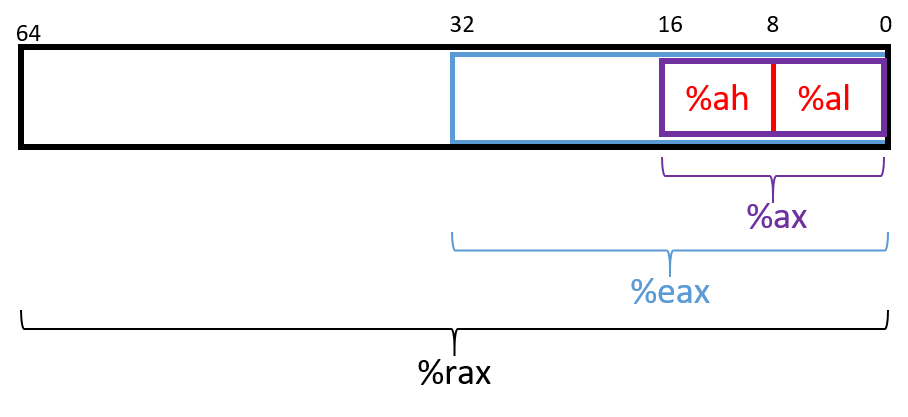
\includegraphics[scale=0.6]{img/register_subsets.png}
      \caption{The names that refer to subsets of register \texttt{\%rax}.} 
      \label{fig:register_subsets}
    \end{figure}
    A complete list is shown below. 
    \begin{table}[H]
      \centering
      \begin{tabular}{|l|l|l|l|}
      \hline
      \textbf{64-bit Register} & \textbf{32-bit Register} & \textbf{Lower 16 Bits} & \textbf{Lower 8 Bits} \\ \hline
      \%rax & \%eax & \%ax & \%al \\ \hline
      \%rbx & \%ebx & \%bx & \%bl \\ \hline
      \%rcx & \%ecx & \%cx & \%cl \\ \hline
      \%rdx & \%edx & \%dx & \%dl \\ \hline
      \%rdi & \%edi & \%di & \%dil \\ \hline
      \%rsi & \%esi & \%si & \%sil \\ \hline
      \%rsp & \%esp & \%sp & \%spl \\ \hline
      \%rbp & \%ebp & \%bp & \%bpl \\ \hline
      \%r8 & \%r8d & \%r8w & \%r8b \\ \hline
      \%r9 & \%r9d & \%r9w & \%r9b \\ \hline
      \%r10 & \%r10d & \%r10w & \%r10b \\ \hline
      \%r11 & \%r11d & \%r11w & \%r11b \\ \hline
      \%r12 & \%r12d & \%r12w & \%r12b \\ \hline
      \%r13 & \%r13d & \%r13w & \%r13b \\ \hline
      \%r14 & \%r14d & \%r14w & \%r14b \\ \hline
      \%r15 & \%r15d & \%r15w & \%r15b \\ \hline
      \end{tabular}
      \caption{Register mapping in x86-64 architecture}
      \label{table:register_mapping}
    \end{table}
  \end{definition}

\subsection{Addressing Modes}

  \begin{example}[Immediate Addressing]
    \begin{lstlisting} 
      movq $0x4, %rax
    \end{lstlisting}
  \end{example}

  \begin{example}[Normal Addressing]
    The following example shows the source operand being a memory address, with normal addressing, and the destination operand being a register.  
    \begin{lstlisting} 
      movq (%rax), %rbx
    \end{lstlisting}
  \end{example}

  \begin{example}[Displacement Addressing]
    The following example shows the source operand being a memory address and the destination operand being a register. They are both addressed normally. 
    \begin{lstlisting} 
      movq 8(%rdi), %rdx
    \end{lstlisting}
  \end{example}

  \begin{example}[Indexed Addressing]
    The following shows the source operand being a memory address and the destination operand being a register. Say that \texttt{\%rdx = 0xf000} and \texttt{\%rcx = 0x0100}. Then 
    \begin{equation}
      \texttt{0x80(,\%rdx,2) = Mem[2*0xF000 + 0x80] = Mem[0x1E080]}
    \end{equation}
    We see that 
    \begin{lstlisting} 
      movq 0x100(%rdi, %rsi, 8), %rdx
    \end{lstlisting}
  \end{example}


\section{x86 Arithmetic Operations} 

  \begin{definition}[Size Specifier]
    In x86 assembly, the \textbf{size specifier} can be appended to this instruction mnemonic to specify the size of the operands. 
    \begin{enumerate} 
      \item \textbf{b} (byte) for 1 byte 
      \item \textbf{w} (word) for 2 bytes
      \item \textbf{l} (long) for 4 bytes 
      \item \textbf{q} (quad word) for 8 bytes
    \end{enumerate}
    Note that due to backwards compatibility, word means 2 bytes in instruction names. Furthermore, the maximum size is 8 bytes since that is the size of each register in x86\_64. 
  \end{definition}

  Like higher level programming languages, we can perform operations, do comparisons, and jump to different parts of the code. Instructions can be generally categorized into three types: 
  \begin{enumerate} 
    \item \textbf{Data Movement}: These instructions move data between memory and registers or between the registery and registery. Memory to memory transfer cannot be done with a single instruction. 
      \begin{lstlisting} 
        %reg = Mem[address]     # load data from memory into register
        Mem[address] = %reg     # store register data into memory
      \end{lstlisting}
    \item \textbf{Arithmetic Operation}: Perform arithmetic operation on register or memory data. 
      \begin{lstlisting} 
        %reg = %reg + Mem[address]     # add memory data to register
        %reg = %reg - Mem[address]     # subtract memory data from register
        %reg = %reg * Mem[address]     # multiply memory data to register
        %reg = %reg / Mem[address]     # divide memory data from register
      \end{lstlisting}
    \item \textbf{Control Flow}: What instruction to execute next. 
      \begin{lstlisting} 
        jmp label     # jump to label
        je label      # jump to label if equal
        jne label     # jump to label if not equal
        jg label      # jump to label if greater
        jl label      # jump to label if less
        call label    # call a function
        ret           # return from a function
      \end{lstlisting}
  \end{enumerate}

  Now unlike compiled languages, which are translated into machine code by a compiler, assembly code is translated into machine code through a two-step process. First, we \textbf{assemble} the assembly code into an \textbf{object file} by an \textbf{assembler}, and then we \textbf{link} the object file into an executable by a \textbf{linker}. Some common assemblers are \textbf{NASM} (Netwide Assembler) and \textbf{GAS/AS} (GNU Assembler), and common linkers are \textbf{ld} (GNU Linker) and \textbf{lld} (LLVM Linker), both installable with \textbf{sudo pacman -S nasm ld}. 

  \begin{definition}[mov]
    Let's talk about the \texttt{mov} instruction. A good diagram to see is the following: 
    \begin{center}  
      % 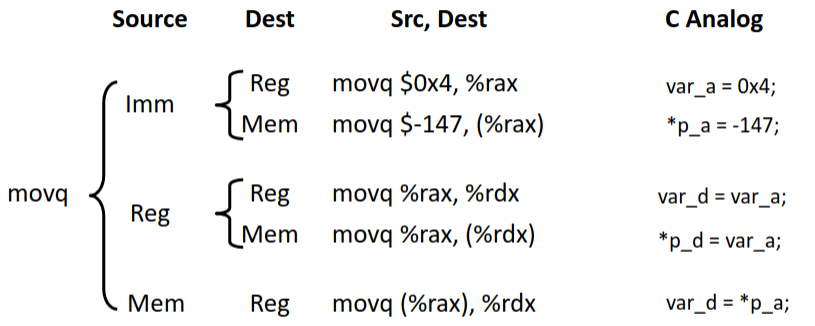
\includegraphics[scale=0.5]{img/movq.png}
    \end{center} 
    Parantheses indicate that we are using a pointer dereference. 
  \end{definition}

  \begin{definition}[int]
    The \texttt{int} instruction is used to generate a software interrupt. It is often used to invoke a system call.
  \end{definition}

  \begin{definition}[ret]
    The \texttt{ret} instruction is used to return from a function. It returns the value in the \texttt{\%rax} register. 
  \end{definition}

  \begin{example}[Swap Function]
    In \textbf{gdb}, we may have a function that swaps two integers. 
    \begin{lstlisting} 
      swap:
        movq (%rdi), %rax
        movq (%rsi), %rdx
        movq %rdx, (%rdi)
        movq %rax, (%rsi)
        ret
    \end{lstlisting}
    which is the assembly code for the following C code.
    \begin{lstlisting} 
      void swap(long *xp, long *yp) {
        long t0 = *xp;
        long t1 = *yp;
        *xp = t1;
        *yp = t0;
      }
    \end{lstlisting}
  \end{example}

  Let's talk about moving instructions first. 

  \begin{definition}[mov]
    Let's talk about the \texttt{mov} instruction which copies data from the source to the destination (the data in the source still remains!) and has the syntax 
    \begin{equation}
      \texttt{mov\_ src, dest}
    \end{equation}
    \begin{enumerate}
      \item The source can be a register (\texttt{\%rsi}), a value (\texttt{\$0x4}), or a memory address (\texttt{0x4}).
      \item The destination can be a register or a memory address. 
      \item The \texttt{\_} is defined to be one of the size operands, which determine how big the data is. For example, we can call \texttt{movq} to move 8 bytes of data (which turns about to be the maximum size of a register). 
    \end{enumerate}
    A good diagram to see is the following: 
    \begin{center}  
      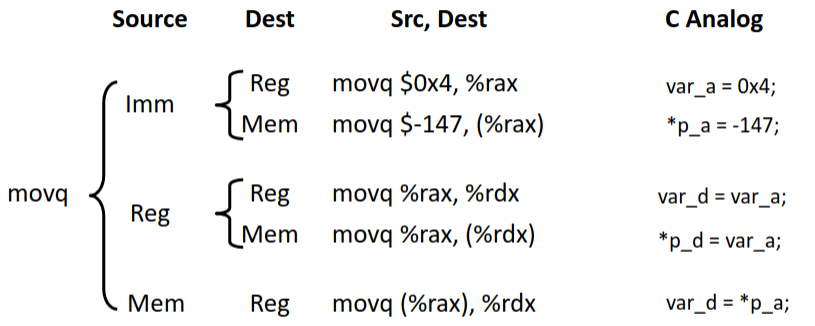
\includegraphics[scale=0.5]{img/movq.png}
    \end{center} 
  \end{definition}

  Even with just the mov instruction, we can look at a practical implementation of a C program in Assembly. 

  \begin{example}[Swap Function]
    Let us take a look at a function that swaps two integers. Let's see what they do. 
    \begin{enumerate}
      \item In C, we dereference both \texttt{xp} and \texttt{yp} (note that they are pointers to longs, so they store 8 bytes), and assign these two values to two temporary variables. Then, we assign the value of \texttt{yp} to \texttt{xp} and the value of \texttt{xp} to \texttt{yp}.
      \item In Assembly, we first take the registers \texttt{\%rdi} and \texttt{\%rsi}, which are the 1st and 2nd arguments of the function, dereference them with the parantheses, and store them in the temporary registers \texttt{\%rax} and \texttt{\%rdx}. Then, we store the value of \texttt{\%rdx} into the memory address of \texttt{\%rdi} and the value of \texttt{\%rax} into the memory address of \texttt{\%rsi}. Note that the input values (the actual of )
    \end{enumerate}

    \noindent\begin{minipage}{.5\textwidth}
    \begin{lstlisting}[]{Code}
      void swap(long *xp, long *yp) {
        long t0 = *xp;
        long t1 = *yp;
        *xp = t1;
        *yp = t0;
      }
    \end{lstlisting}
    \end{minipage}
    \hfill
    \begin{minipage}{.49\textwidth}
    \begin{lstlisting}[]{Output}
      swap:
        movq (%rdi), %rax
        movq (%rsi), %rdx
        movq %rdx, (%rdi)
        movq %rax, (%rsi)
        ret
    \end{lstlisting}
    \end{minipage}
  \end{example}

  \begin{definition}[movz and movs]
    The \texttt{movz} and \texttt{movs} instructions are used to move data from the source to the destination, but with zero and sign extension, respectively. It is used to copy from a smaller source value to a larger destination, with the syntax 
    \begin{align*}
      \texttt{movz\_\_ src, dest} \\ 
      \texttt{movs\_\_ src, dest} 
    \end{align*}
    where the first $\_$ is the size of the source and the second $\_$ is the size of the destination. 
    \begin{enumerate}
      \item The source can be from a memory or register. 
      \item The destination must be a register. 
    \end{enumerate}
  \end{definition}

  \begin{example}[Simple example with movz]
    Take a look at the code below. 
    \begin{lstlisting}
      movzbq %al, %rbx
    \end{lstlisting}
    The \texttt{\%al} represents the last byte of the \texttt{\%rax} register. It is 1 byte long. The \texttt{\%rbx} register is 8 bytes long, so we can fill in the rest of the 7 bytes with zeros. 
    \begin{center}  
      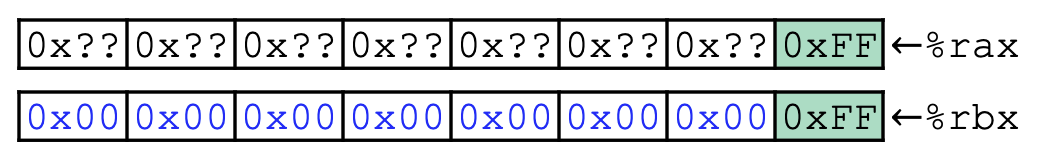
\includegraphics[scale=0.5]{img/movzbq.png}
    \end{center}
  \end{example}

  \begin{example}[Harder example with movs]
    Take a look at the code below. 
    \begin{lstlisting}
      movsbl (%rax), %ebx
    \end{lstlisting}
    You want to move the value at the memory address in \texttt{\%rax} into \texttt{\%ebx}. Since the source size is set to 1 byte, you take that byte, say it is \texttt{0x80}, from the memory, and then sign extend it (by a size of 4 bytes!) into \texttt{\%ebx}. Note that therefore, the first four bytes of \texttt{\%rbx} will not be affected since it's not a part of \texttt{\%ebx}. An exception to this is that in x86-64, any instruction that generates a 32-bit long word value for a register also sets the high-order 32 bits of the register to 0, so this ends up clearing the first 4 bytes to 0. 
    \begin{center}  
      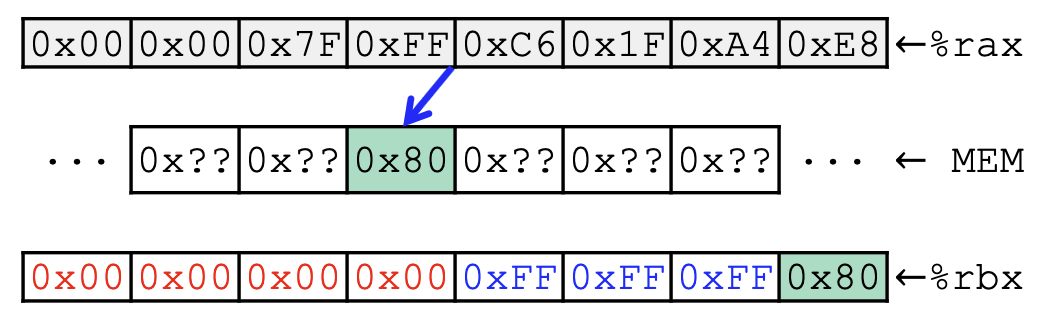
\includegraphics[scale=0.5]{img/movsbl.png}
    \end{center}
  \end{example}

  Now we can talk about control transfer. Say that you have the following C and Assembly code. 
  
  \begin{figure}[H]
    \centering 
    \noindent\begin{minipage}{.5\textwidth}
    \begin{lstlisting}[]{Code}
      int add(int x) {
        return x + 2; 
      }

      int main() {
        int a = 2; 
        int b = add(a); 
        return 0; 
      }
    \end{lstlisting}
    \end{minipage}
    \hfill
    \begin{minipage}{.49\textwidth}
    \begin{lstlisting}[]{Output}
      add: 
        movq %rdi, %rax 
        addq $2, %rax 
        ret 
      main:
        movq $3, $rdi 
        call add 
        movq $0, %rax 
        ret 
    \end{lstlisting}
    \end{minipage}
    \caption{A simple function. } 
    \label{fig:stack_example}
  \end{figure}

  If you go through the instructions, you see that in main, you first move \texttt{\$3} into the \texttt{\%rdi} register. Then, you call the \texttt{add} function, and within it you also have the \texttt{\%rdi} register. This is a conflict in the register, and we don't want to simply overwrite the value of \texttt{\%rdi} in the \texttt{main} function. Simply putting it to another register isn't a great idea since we can't always guarantee that it will be free. Therefore, we must use the memory itself. 

  Recall the stack, which we can think of as a giant array in which data gets pushed and popped in a last-in-first-out manner. The stack is used to store data and return addresses, and is used to manage function calls. Visually, we want to think of the elements getting pushed in from the bottom (upside down) towards lower memory addresses. 

  \begin{definition}[Stack Pointer]
    Note that every time we want to push or pop something from the stack, we must know \textit{where} to push or pop it. This is where the \textbf{stack pointer} comes in. It is a special register that always points to the top of the stack, and is used to keep track of the stack.
  \end{definition}

  \begin{definition}[Push and Pop]
    The \texttt{push} and \texttt{pop} instructions are used to push and pop data onto and off the stack, respectively. 
    \begin{align*}
      \texttt{push\_ src} && \texttt{rsp = rsp - 8; Mem[rsp] = src} \\
      \texttt{pop\_ dest} && \texttt{dest = Mem[rsp]; rsp = rsp + 8} 
    \end{align*}
    \begin{enumerate}
      \item When we push the source, we fetch the value at the source and store it at the memory address pointed to by the stack pointer \texttt{\%rsp}. Then, we decrement \texttt{\%rsp} by 8.
      \item When we pop from the stack, we fetch the value at the memory address pointed to by the stack pointer \texttt{\%rsp} and store it in the destination. Then, we increment \texttt{\%rsp} by 8.
    \end{enumerate}
    Note that no matter what the size of the operand, we always subtract 8 from the stack pointer. This is because the stack grows downwards, and we want to make sure that the next element is pushed into the next available space.
  \end{definition}

  Note that the register \texttt{\%rsp} is the stack pointer, which points to the top of the stack. The stack is used to store data and return addresses, and is used to manage function calls. 

  \begin{definition}[Push and Pop]
    The \texttt{push} and \texttt{pop} instructions are used to push and pop data onto and off the stack, respectively. 
    \begin{align*}
      \texttt{push\_ src} && \texttt{rsp = rsp - 8; Mem[rsp] = src} \\
      \texttt{pop\_ dest} && \texttt{dest = Mem[rsp]; rsp = rsp + 8} 
    \end{align*}
    The \texttt{\_} is a size operand, which determines how big the data is.
  \end{definition}

  \begin{definition}[Call and Ret]
    The \texttt{call} instruction pushes the return address onto the stack and jumps to the function. The \texttt{ret} instruction pops the return address from the stack and jumps to it.
  \end{definition}

  We also talked about how there is instruction code that is even below the stack that is stored. This is where all the machine code/assembly is stored, and we want to find out where we are currently at in this code. This is done with the program counter. 

  \begin{definition}[Program Counter, Instruction Pointer] 
    The \textbf{program counter}, or \textbf{instruction pointer}, is a special register \textbf{rip} that points to the current instruction in the program. It is used to keep track of the next instruction to be executed.
  \end{definition}

  Let's go through one long example to see in detail how this is calculated. 
  
  \begin{example}[Evaluating a Function]
    Say that we have the following C code. 
    \begin{lstlisting}
      int adder2(int a) {
        return a + 2; 
      }

      int main() {
        int x = 40; 
        x = adder2(x); 
        printf("x is: %d\n", x);
        return 0; 
      }
    \end{lstlisting}
    When we compile this program, we can view its full assembly code by calling \texttt{objdump -d a.out}. The output is quite long, so we will focus on the instruction for the \texttt{adder2} function. 
    \begin{figure}[H]
      \centering 
      \begin{lstlisting}
        0000000000400526 <adder2>:
        400526:       55                      push   %rbp
        400527:       48 89 e5                mov    %rsp,%rbp
        40052a:       89 7d fc                mov    %edi,-0x4(%rbp)
        40052d:       8b 45 fc                mov    -0x4(%rbp),%eax
        400530:       83 c0 02                add    $0x2,%eax
        400533:       5d                      pop    %rbp
        400534:       c3                      retq
      \end{lstlisting}
      \caption{The output of objdump for the \texttt{adder2} function. The leftmost column represents the addresses (in hex) of where the actual instructions lie. The second column represents the machine code that is being executed. The third column represents the assembly code.}
      \label{fig:adder2} 
    \end{figure}
    Note some things. Since \texttt{adder2} is taking in an integer input value, we want to load it into the lower 32 bits (4 bytes) of the \texttt{\%rdi} register, which is the first parameter. So we use \texttt{\%edi}. Likewise for the return value, we want to output an int so we use \texttt{\%eax} rather than \texttt{\%rax}. Let's go through some of the steps. 
    \begin{enumerate}
      \item By the time we get into calling \texttt{adder2}, we can take a look at the relevant registers. 

        \begin{center}
          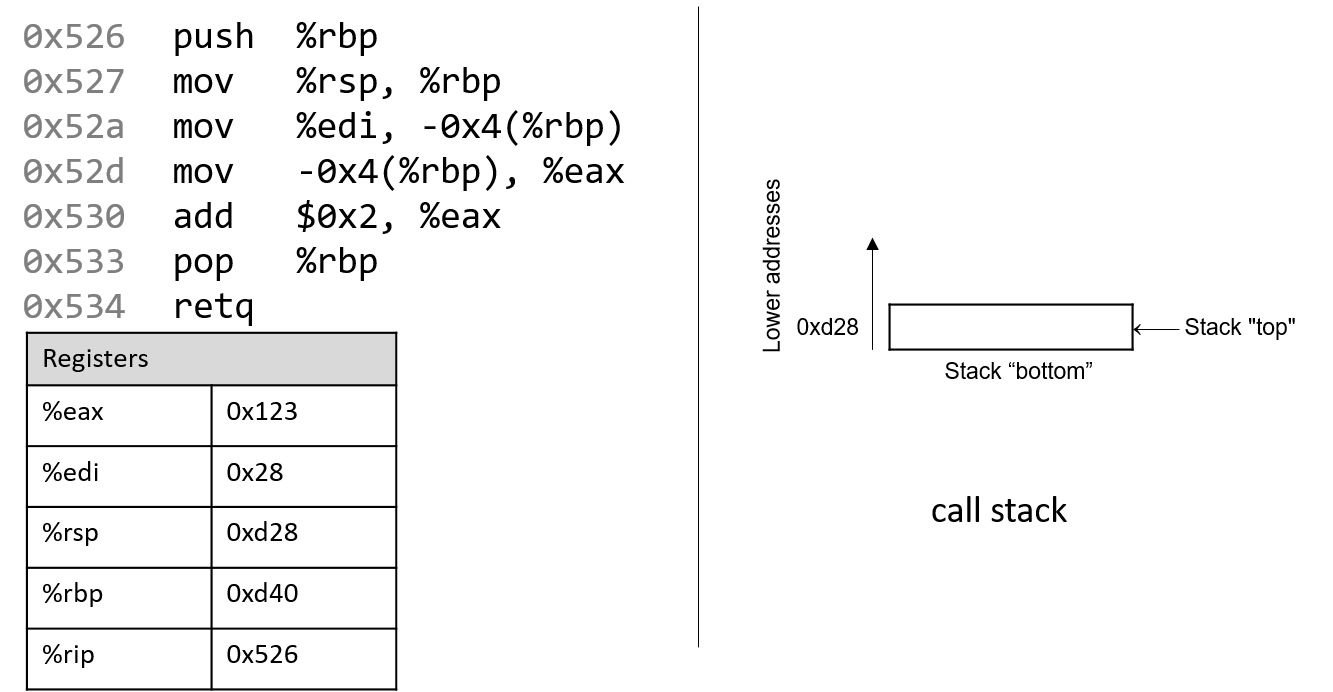
\includegraphics[scale=0.5]{img/ex1_1.png}
        \end{center}
        \begin{enumerate}
          \item First, the \texttt{\%eax} is filled with garbage, which are leftovers from previous programs that haven't been overwritten yet. 
          \item Second, the \texttt{\%edi=0x28} since we have set \texttt{x=40} in \texttt{main}, before calling \texttt{adder2}, so it lingers on. 
          \item \texttt{\%rsp=0xd28} since that is where the top of the stack is. 
          \item \texttt{\%rbp=0xd40} 
          \item \texttt{\%rip=0x526} since that is where we are currently at in our instruction (we are about to do it, but haven't done it yet). 
        \end{enumerate}

      \item When we execute the first line of code, we simply push the value at \texttt{\%rbp} into the stack. The top of the stack gets decremeneted by 8 and the value at \texttt{\%rbp} is stored there. This means that the top of the stack is at \texttt{\%rsp=0xd20} and the next instruction will be at \texttt{\%rip=0x527}.  

        \begin{center}
          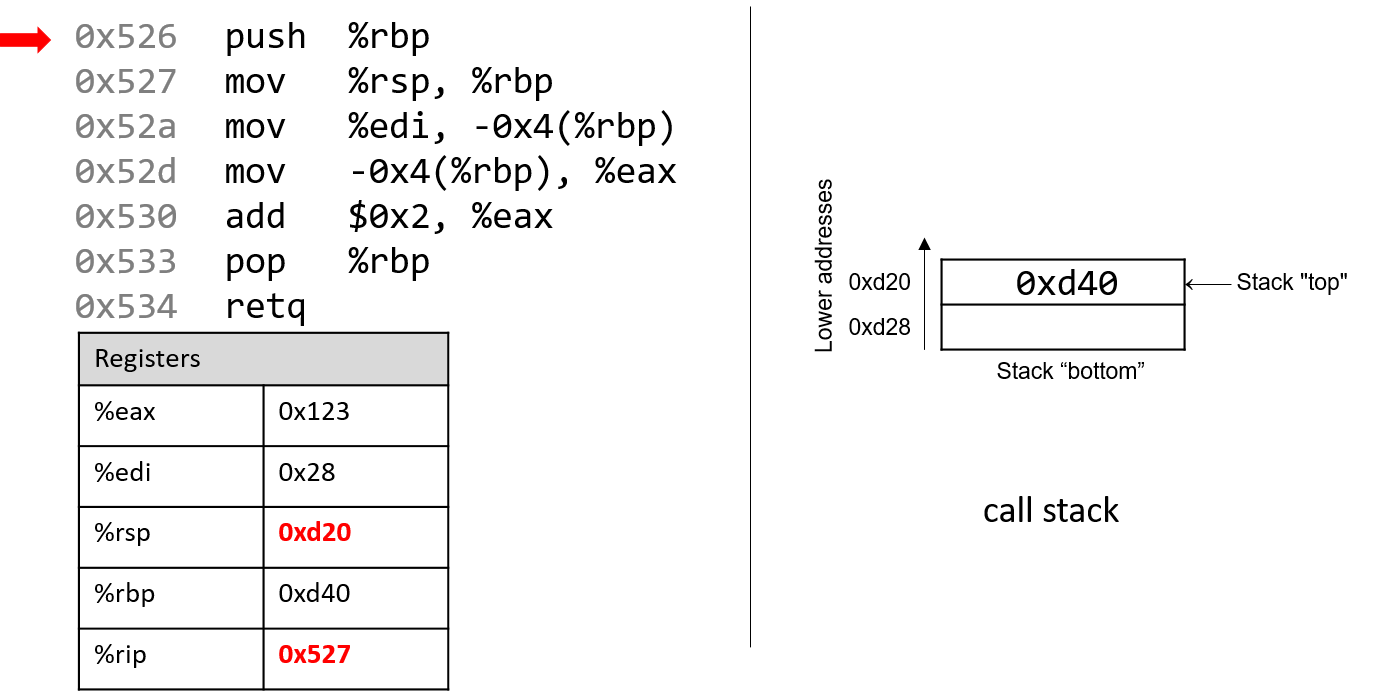
\includegraphics[scale=0.5]{img/ex1_2.png}
        \end{center}

      \item The reason we have pushed \texttt{\%rbp} onto the stack is that we want to save it before it gets overwritten by this next execution. We basically move the value of \texttt{\%rsp} into \texttt{\%rbp}, and the \texttt{\%rip} advances to the next instruction. \texttt{\%rip} moves to the next instruction. 

        \begin{center}
          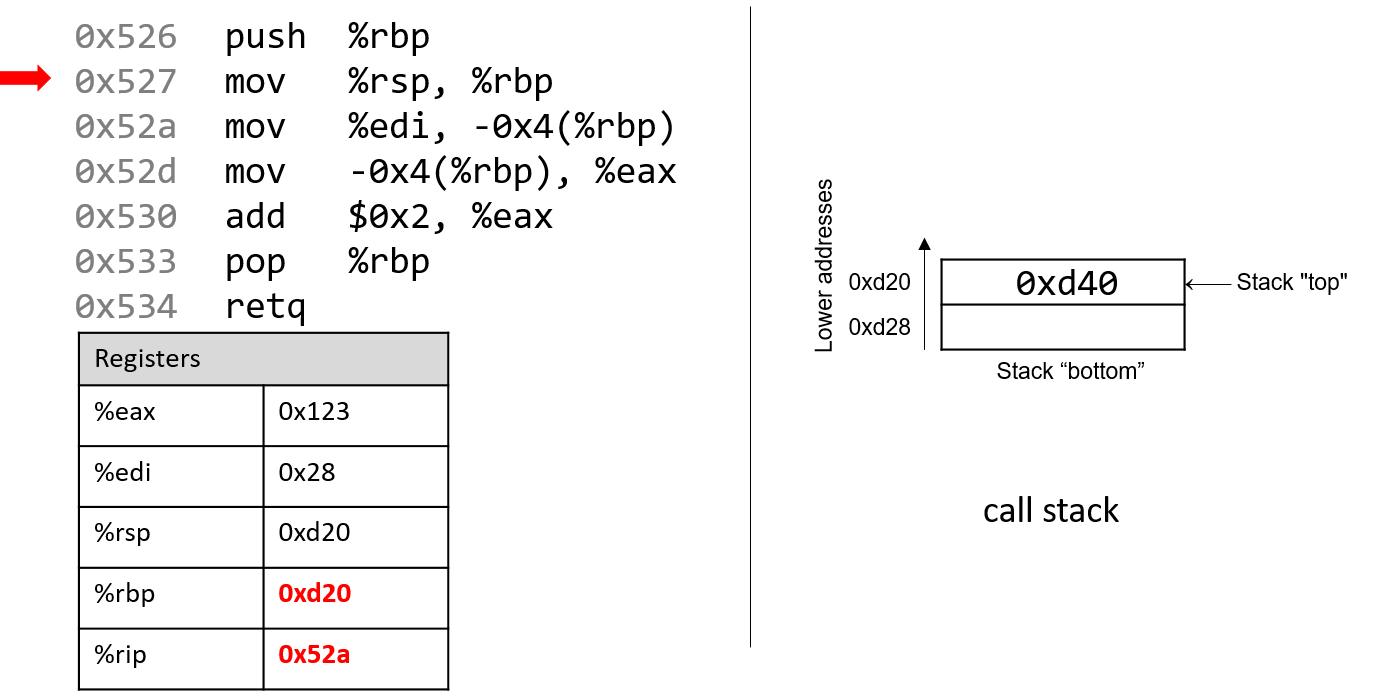
\includegraphics[scale=0.5]{img/ex1_3.png}
        \end{center}

      \item Now we want to take our first argument \texttt{\%edi} and store it in memory. Note that since this is 4 bytes, we can move this value into memory that is 4 bytes below the stack (\texttt{-0x4(\%rbp)}). Note that the storing the value of \texttt{\%edi} into memory doesn't affect the stack pointer \texttt{\%rsp}. As far as the program is concerned, the top of this stack is still address \texttt{0xd20}. 

        \begin{center}
          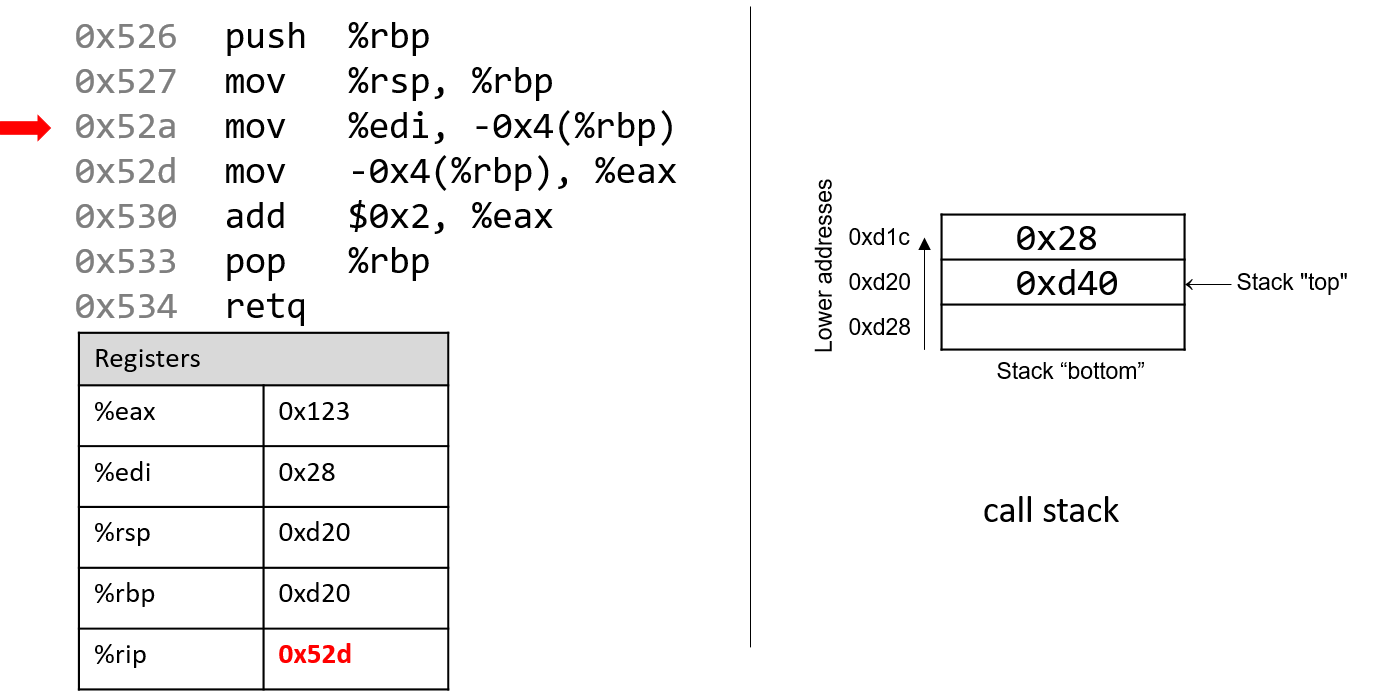
\includegraphics[scale=0.5]{img/ex1_4.png}
        \end{center}

      \item The next instruction simply goes into memory 4 bytes below the stack pointer, takes the value there, and stores it into \texttt{\%eax}. This is the value of \texttt{\%edi} that we just stored. This may seem redundant since we are making a round trip to memory and back to ultimately move the value of \texttt{\%edi} into \texttt{\%eax}, but compilers are not smart and just follow these instructions. 

        \begin{center}
          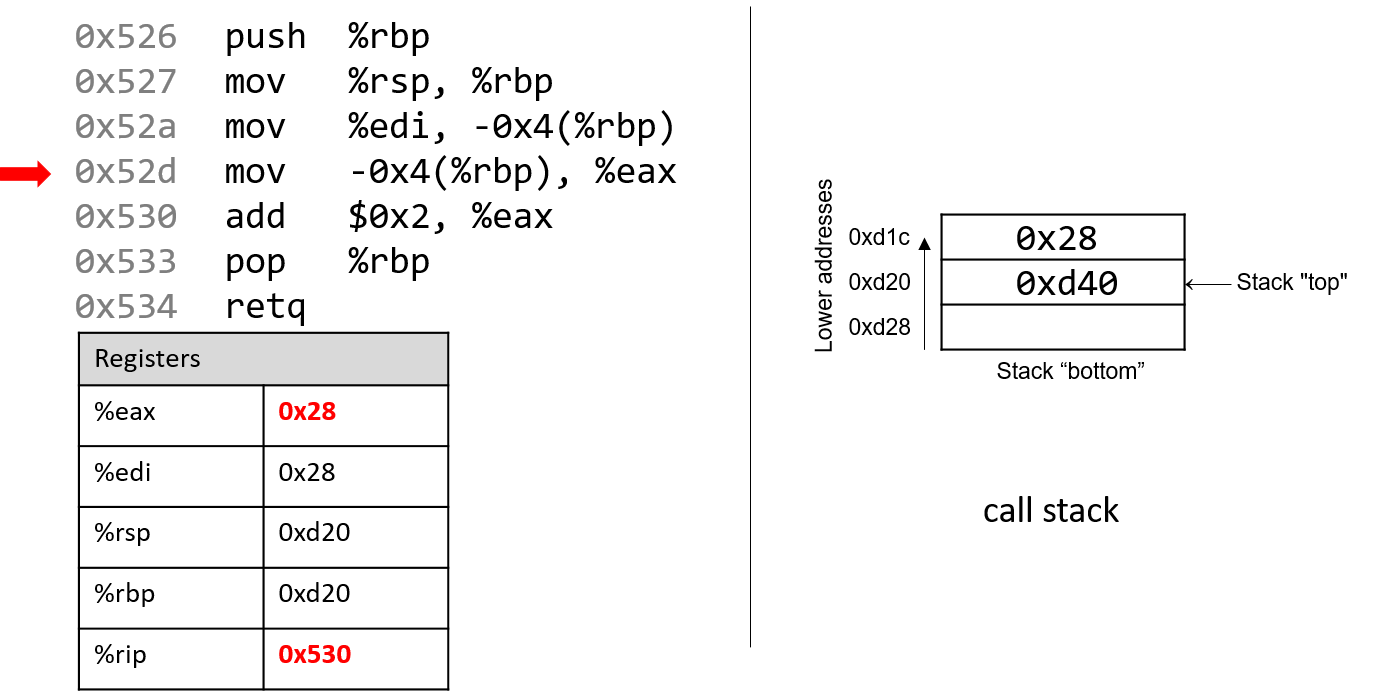
\includegraphics[scale=0.5]{img/ex1_5.png}
        \end{center}

      \item Finally, we add the value \texttt{\$0x2} to \texttt{\%eax} and store it back into \texttt{\%eax}. 

        \begin{center}
          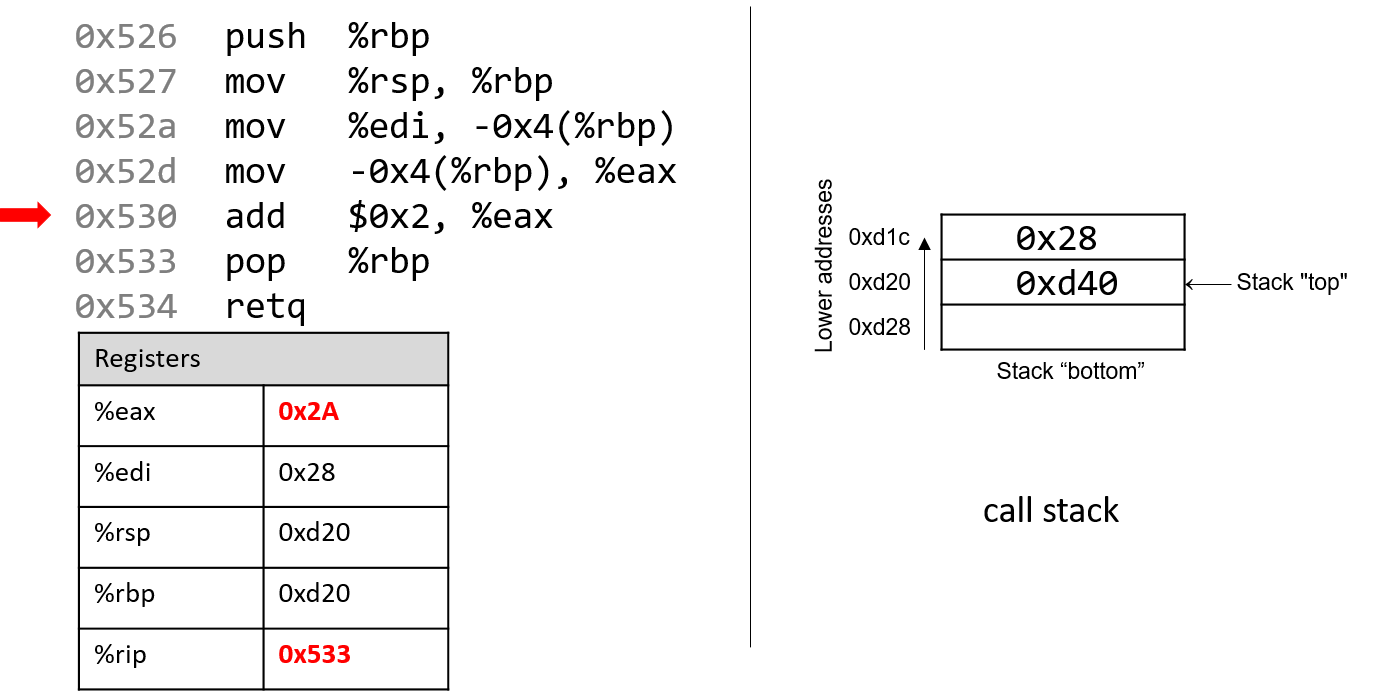
\includegraphics[scale=0.5]{img/ex1_6.png}
        \end{center}

      \item Finally, we pop the value at the top of the stack and store it into \texttt{\%rbp}. Note that this is \textit{not} the value \texttt{0x28}. It is simply the value that is stored at \texttt{\%rsp=0xd20}, which is \texttt{(\%rsp)=0xd40}. 

        \begin{center}
          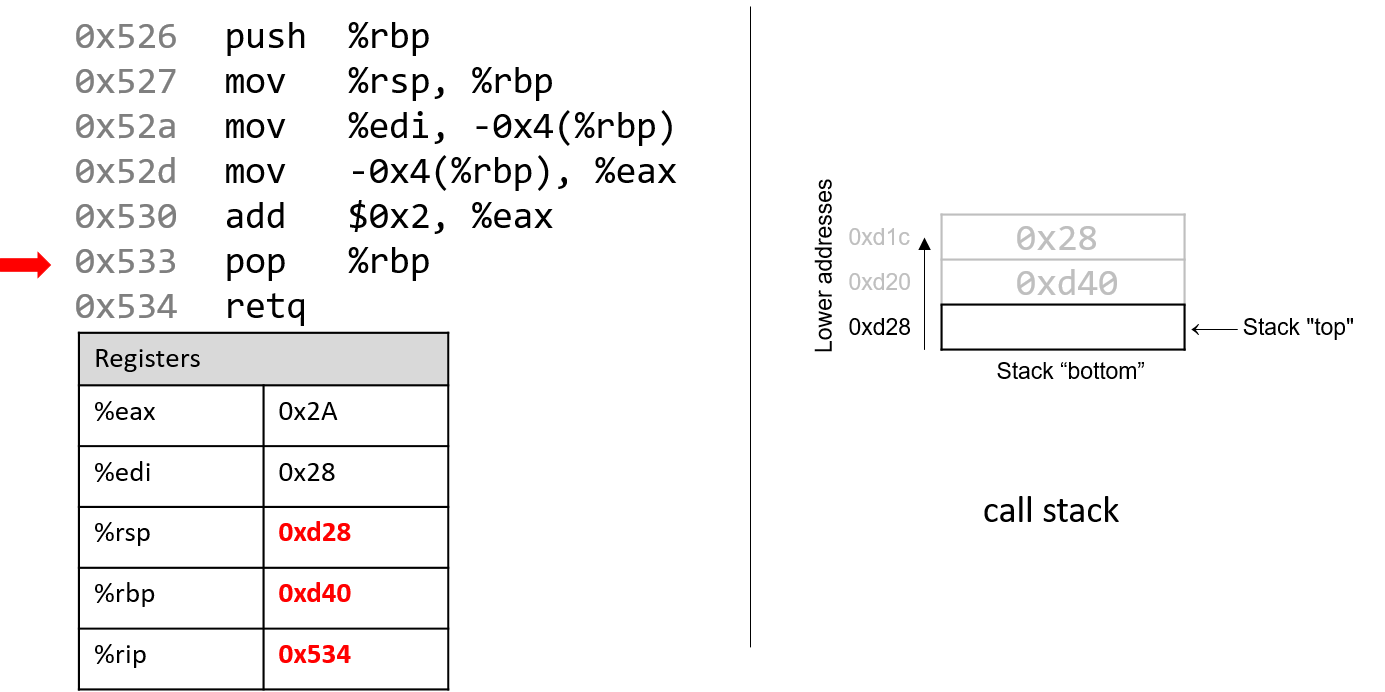
\includegraphics[scale=0.5]{img/ex1_7.png}
        \end{center}

      \item Finally, we return the value with \texttt{retq}. 
    \end{enumerate}
  \end{example}

  Note that the final values in the registers \texttt{\%rsp} and \texttt{\%rip} are \texttt{0xd28} and \texttt{0x534}, respectively, which are the same values as when the function started executing! This is normal and expected behavior with the call stack, which just stores temporary variable sand data of each function as it executes a program. Once a function completes executing, the stack returns to the state it was in prior to the function call. Therefore, it is common to see the following two instructions at the beginning of a function: 
  \begin{lstlisting}
    push %rbp 
    mov %rsp, %rbp
  \end{lstlisting}
  and the following two at the end of a function 
  \begin{lstlisting}
    pop %rbp 
    retq
  \end{lstlisting}

  Now arithemtic operations are quite simple.

  \begin{definition}[Add, Subtract, Multiply]
    The \textbf{add} and \textbf{sub} instructions are used to add and subtract data from the destination. 
    \begin{align*}
      \texttt{add\_ src, dest} && \texttt{dest = dest + src} \\
      \texttt{sub\_ src, dest} && \texttt{dest = dest - src}
    \end{align*}
    The \textbf{imul} instruction is used to multiply data between the source and destination and store it in the destination.  
    \begin{align*}
      \texttt{imul\_ src, dest} && \texttt{dest = dest * src} 
    \end{align*}
    Again the \texttt{\_} is a size operand, which determines how big the data is. 
  \end{definition}

  \begin{definition}[Increment, Decrement]
    The \textbf{inc} and \textbf{dec} instructions are used to increment and decrement the value in the destination. 
    \begin{align*}
      \texttt{inc\_ dest} && \texttt{dest = dest + 1} \\
      \texttt{dec\_ dest} && \texttt{dest = dest - 1}
    \end{align*}
  \end{definition}

  \begin{definition}[Negative]
    The \textbf{neg} instruction is used to negate the value in the destination. 
    \begin{align*}
      \texttt{neg\_ dest} && \texttt{dest = -dest} 
    \end{align*}
  \end{definition}

  \begin{example}[Basic Arithmetic Function]
    The following represents the same program in C and in assembly. Let's go through each one: 
    \begin{enumerate}
      \item In C, we first initialize \texttt{a = 4}, then \texttt{b = 8}, add them together to get \texttt{c}, and then return \texttt{c}.
      \item In Assembly, we move the value $4$ to the \texttt{\%rax} register, then move the value $8$ to the \texttt{\%rbx} register, add the two values together to store it into \texttt{\%rax}, and then return the value in the \texttt{\%rax} register.
    \end{enumerate}
    \noindent\begin{minipage}{.5\textwidth}
    \begin{lstlisting}[]{Code}
      int main() {
        int a = 4, b = 8; 
        int c = a + b; 
        return c; 
      }
    \end{lstlisting}
    \end{minipage}
    \hfill
    \begin{minipage}{.49\textwidth}
    \begin{lstlisting}[]{Output}
      main:
        movq $4, %rax
        movq $8, %rbx
        addq %rbx, %rax
        ret
    \end{lstlisting}
    \end{minipage}
    It is slightly different in Assembly since rather than storing $4$ in some intermediate register, we immediately store it in the return register. In a way it is more optimized, and this is what the compiler does for you so that as few registers are used. 
  \end{example}

  A shorthand way to do this is with \texttt{lea}, which stands for load effective address. 

  \begin{definition}[Load Effective Address]
    The \textbf{lea} instruction is used to load the effective address of the source into the destination. For now, we will focus on the arithmetic operations that it can do
    \begin{align*}
      \texttt{lea\_ (src1, src2), dest} && \texttt{dest = src1 + src2}  \\ 
      \texttt{lea\_ (src1, src2, scale), dest} && \texttt{dest = src1 + src2*scale}  \\ 
      \texttt{lea\_ const(src1, src2), dest} && \texttt{dest = src1 + src2 + const} \\ 
      \texttt{lea\_ const(src1, src2, scale), dest} && \texttt{dest = src1 + src2*scale + const}
    \end{align*}
    This is useful for doing arithmetic operations on the address of a variable.
  \end{definition}

  \begin{definition}[Bitwise]
    The \textbf{and}, \textbf{or}, \textbf{xor}, and \textbf{not} instructions are used to perform bitwise operations on the source and destination. 
    \begin{align*}
      \texttt{and src, dest} && \texttt{dest = dest \& src}  \\
      \texttt{or src, dest} && \texttt{dest = dest | src}  \\
      \texttt{xor src, dest} && \texttt{dest = dest \^ src}  \\
      \texttt{neg dest} && \texttt{dest = -dest}  \\
      \texttt{not dest} && \texttt{dest = $\sim$dest}  
    \end{align*}
  \end{definition}

  \begin{definition}[Arithmetic and Logical Bit Shift]
    The \texttt{sal} arithmetic instruction is used to shift the bits of the destination to the left by the number of bits specified in the source. The \texttt{shr} instruction is used to shift the bits of the destination to the right by the number of bits specified in the source.
    \begin{align*}
      \texttt{sal src, dest} && \texttt{dest = dest << src}  \\
      \texttt{shr src, dest} && \texttt{dest = dest >> src}
    \end{align*}
    The \texttt{sar} instruction is used to shift the bits of the destination to the right by the number of bits specified in the source, and fill the leftmost bits with the sign bit. The \texttt{shl} instruction is used to shift the bits of the destination to the left by the number of bits specified in the source, and fill the rightmost bits with zeros. 
    \begin{align*}
      \texttt{sar src, dest} && \texttt{dest = dest >> src}  \\
      \texttt{shl src, dest} && \texttt{dest = dest << src}
    \end{align*}
  \end{definition}

  \begin{example}[Harder Arithmetic Example]
    The following two codes are equivalent. 

    \noindent\begin{minipage}{.5\textwidth}
    \begin{lstlisting}[]{Code}
      long arith(long x, long y, long z) {
        long t1 = x + y; 
        long t2 = z + t1; 
        long t3 = x + 4; 
        long t4 = y * 48; 
        long t5 = t3 + t4;
        long rval = t2 * t5; 
        return rval; 
      }
      .
      .
      .
      .
      .
    \end{lstlisting}
    \end{minipage}
    \hfill
    \begin{minipage}{.49\textwidth}
    \begin{lstlisting}[]{Output}
      arith: 
        # rax/t1 = x + y
        leaq  (%rdi, %rsi), %rax
        # rax/t2 = z + t1
        addq  %rdx, %rax
        #rdx = 3 * y 
        leaq  (%rsi, %rsi, 2), %rdx
        #rdx/t4 = (3*y) * 16
        salq  $4, %rdx 
        #rcx/t5 = x + t4 + 4
        leaq  4(%rdi, %rdi), %rcx 
        # rax/rval = t5 * t2
        imulq %rcx, %rax 
        ret 
    \end{lstlisting}
    \end{minipage}
  \end{example}

  The final thing in our list is condition codes. 

  Sometimes, we want to move (really copy) some value to another register if some condition is met. This is where we use conditional moves. These conditions are met by the flags register, which is a special register that stores the status of the last operation. It is the value of these flags that determine whether all future conditional statements are met in assembly. 
  
  \begin{definition}[Condition Code Flags]
    The flags register in the x86 CPU keeps 4 \textit{condition code} flag bits internally. Think of these as status flags that are \textit{implicitly} set by the most recent arithmetic operation (think of it as side effects). Note that condition codes are NOT set by \texttt{lea} or \texttt{mov} instructions! 
    \begin{enumerate}
      \item \textbf{Zero Flag}: if the last operation resulted in a zero value.
      \item \textbf{Sign Flag}: if the last operation resulted in a negative value (i.e. the most significant bit is 1).
      \item \textbf{Overflow Flag}: if the last operation resulted in a signed overflow.
      \item \textbf{Carry Flag}: if the last operation resulted in a carry out of the most significant bit, i.e. an unsigned overflow. 
    \end{enumerate}
    Every operation may or may not changes these flags to test for zero or nonzero, positive or negative, or overflow conditions, and combinations of these flags express the full range of conditions and cases, e.g. for signed and unsigned values. 
  \end{definition}

  \begin{example}[Zero Flag]
    If the code below was just run, then ZF would be set to 1. 
    \begin{lstlisting}
      movq $2, %rax 
      subq $2, %rax
    \end{lstlisting}
  \end{example}

  \begin{example}[Sign Flag]
    If the code below was just run, then SF would be set to 1. 
    \begin{lstlisting}
      movq $2, %rax 
      subq $4, %rax
    \end{lstlisting}
  \end{example}

  \begin{example}[Overflow Flag]
    If either code below was just run, then OF would be set to 1. 

    \noindent\begin{minipage}{.5\textwidth}
    \begin{lstlisting}[]{Code}
      movq $0x7fffffffffffffff, %rax 
      addq $1, %rax
    \end{lstlisting}
    \end{minipage}
    \hfill
    \begin{minipage}{.49\textwidth}
    \begin{lstlisting}[]{Output}
      movq 0x8000000000000000, %rax 
      addq 0xffffffffffffffff, %rax
    \end{lstlisting}
    \end{minipage}
    This is because in the left in signed arithmetic, we have a positive + positive = negative (result is \texttt{0x8000000000000000}), which is a signed overflow. Furthermore, in the right we have negative + negative = positive (result is \texttt{0x7fffffffffffffff}). 
  \end{example}

  \begin{example}[Carry Flag]
    If the code below was just run, then CF would be set to 1. 
    \begin{lstlisting}
      movq $0xffffffffffffffff, %rax 
      addq $1, %rax
    \end{lstlisting}
    This is because the result is $0x0$, which is a carry out of the most significant bit and an unsigned overflow.
  \end{example}

  It would be tedious to always set these flags manually, so there are two methods that can be used to \textit{explicitly} set these flags. 

  \begin{definition}[Compare]
    The \textbf{cmp} instruction is used to perform a subtraction between the source and destination, and set the flags accordingly, but it does not store the result.
    \begin{align*}
      \texttt{cmp\_ src, dest} && \texttt{dest - src} 
    \end{align*}
    The following flags are set if the conditions are met: 
    \begin{enumerate}
      \item \textbf{ZF = 1} if \texttt{dest == src} 
      \item \textbf{SF = 1} if \texttt{dest < src} (MSB is 1) 
      \item \textbf{OF = 1} if signed overflow 
      \item \textbf{CF = 1} if unsigned overflow
    \end{enumerate}
  \end{definition}

  \begin{definition}[Test]
    The \textbf{test} instruction is used to perform a bitwise AND operation between the source and destination, and set the flags accordingly. 
    \begin{align*}
      \texttt{test\_ src, dest} && \texttt{dest \& src} 
    \end{align*}
    The following flags are set if the conditions are met. Note that you can't have carry out (CF) or overflow (OF) if these flags are set. 
    \begin{enumerate}
      \item \textbf{ZF = 1} if \texttt{dest \& src == 0} 
      \item \textbf{SF = 1} if \texttt{dest \& src < 0} (MSB is 1) 
    \end{enumerate}
  \end{definition}

  \begin{example}[Compare] 
    Assuming that \texttt{\%al = 0x80} and \texttt{\%bl = 0x81}, which flags are set when we execute \texttt{cmpb \%al, \%bl}? Well we must first compute 
    \begin{equation}
      \texttt{\%bl - \%al = 0x81 - 0x80 = 0x81 + $\sim$ 0x80 + 1 = 0x81 + 0x7F + 1 = 0x101 = 0x01}
    \end{equation}
    \begin{enumerate}
      \item CF=1 since the result is greater than 0xFF (i.e. larger than byte) 
      \item ZF=0 since the result is not 0 
      \item SF=0 since the MSB is 0, i.e. there is unsigned overflow
      \item OF=0 since there is no signed overflow
    \end{enumerate}
  \end{example}

  For conditional moves and jumps later shown, it basically uses these explicit sets and always compares them to $0$. We will see what this means later. 

  Finally, we can actually set a byte in a register to 1 or 0 based on the value of a flag. 

  \begin{definition}[Set]
    
  \end{definition}

  We can then talk about conditional moves and jumps.  

  \begin{definition}[Equality with 0]
    The \texttt{test} instruction is used to perform a bitwise AND operation between the source and destination, and set the flags accordingly. 
    \begin{align*}
      \texttt{test\_ src, dest} && \texttt{dest \& src} 
    \end{align*}
    The \texttt{sete} instruction is used to set the destination to 1 if the zero flag is set, and 0 otherwise. 
    \begin{align*}
      \texttt{sete\_ dest} && \texttt{dest = (ZF == 1) ? 1 : 0} 
    \end{align*}
    The \texttt{cmovne} instruction is used to move the source to the destination if the zero flag is not set. 
    \begin{align*}
      \texttt{cmovne\_ src, dest} && \texttt{dest = (ZF == 0) ? src : dest} 
    \end{align*}
  \end{definition}


  \begin{definition}[Jump]
    There are several jump instructions, but essentially they are used to jump to another part of the code. We can use the following mnemonic to jump to a label. 

    \begin{figure}[H]
      \centering 
      \begin{table}[H]
        \centering
        \begin{tabular}{|l|l|}
        \hline
        \textbf{Letter} & \textbf{Word} \\ \hline
        j & jump \\ \hline
        n & not \\ \hline
        e & equal \\ \hline
        s & signed \\ \hline
        g & greater (signed interpretation) \\ \hline
        l & less (signed interpretation) \\ \hline
        a & above (unsigned interpretation) \\ \hline
        b & below (unsigned interpretation) \\ \hline
        \end{tabular}
        \caption{Letter to Word Mapping}
        \label{table:letter_word_mapping}
      \end{table}
      \caption{Mnemonic for Jump Instructions} 
      \label{fig:jump_instructions_mnemonic}
    \end{figure}

    For completeness, we include all the jump instructions. 
      
    \begin{figure}[H]
      \centering 
      \begin{table}[H]
        \centering
        \begin{tabular}{|l|l|l|}
        \hline
        \textbf{Signed Comparison} & \textbf{Unsigned Comparison} & \textbf{Description} \\ \hline
        je (jz) & & jump if equal (==) or jump if zero \\ \hline
        jne (jnz) & & jump if not equal (!=) \\ \hline
        js & & jump if negative \\ \hline
        jns & & jump if non-negative \\ \hline
        jg (jnle) & ja (jnbe) & jump if greater (>) \\ \hline
        jge (jnl) & jae (jnb) & jump if greater than or equal (>=) \\ \hline
        jl (jnge) & jb (jnae) & jump if less (<) \\ \hline
        jle (jng) & jbe (jna) & jump if less than or equal (<=) \\ \hline
        \end{tabular}
        \caption{Comparison Instructions in Assembly}
        \label{table:comparison_instructions}
      \end{table}
      \caption{All jump instructions} 
      \label{fig:jump_instructions_all}
    \end{figure}
  \end{definition}

  \begin{definition}[int]
    The \texttt{int} instruction is used to generate a software interrupt. It is often used to invoke a system call.
  \end{definition}

  \begin{definition}[ret]
    The \texttt{ret} instruction is used to return from a function. It returns the value in the \texttt{\%rax} register. 
  \end{definition}

  Now we can have a basic idea of how if statements can be used as a sequence of conditionals and jump operators. Let's first look at the \textbf{goto} version of C. 

  \begin{definition}[Goto Syntax]
    The goto version processes instructions sequentially as long as there is no jump. This is useful because compilers translating code into assembly designate a jump when a condition is true. Contrast this behavior with the structure of an if statement, where a "jump" (to the else) occurs when conditions are not true. The goto form captures this difference in logic.
  \end{definition}

  \begin{figure}[H]
    \centering 
    \noindent\begin{minipage}{.5\textwidth}
    \begin{lstlisting}[]{Code}
      int getSmallest(int x, int y) {
        int smallest;
        if ( x > y ) { //if (conditional)
          smallest = y; //then statement
        }
        else {
          smallest = x; //else statement
        }
        return smallest;
      }
      .
      .
      .
      .
      .
    \end{lstlisting}
    \end{minipage}
    \hfill
    \begin{minipage}{.49\textwidth}
    \begin{lstlisting}[]{Output}
      int getSmallest(int x, int y) {
        int smallest;

        if (x <= y ) { //if (!conditional)
          goto else_statement;
        }
        smallest = y; //then statement
        goto done;

      else_statement:
        smallest = x; //else statement

      done:
        return smallest;
      }      
    \end{lstlisting}
    \end{minipage}
    \caption{C vs GoTo code of the same function. While GoTo code allows us to view C more like assmebly, it is generally not readable and is not considered best practice. } 
    \label{fig:c_vs_goto}
  \end{figure}

  Now let's see how if statements are implemented by taking a look at this function straight up in assembly. 

  \begin{figure}[H]
    \centering 
    \noindent\begin{minipage}{.4\textwidth}
    \begin{lstlisting}[]{Code}
      int getSmallest(int x, int y) {
        int smallest;
        if ( x > y ) { //if (conditional)
          smallest = y; //then statement
        }
        else {
          smallest = x; //else statement
        }
        return smallest;
      }
      .
    \end{lstlisting}
    \end{minipage}
    \hfill
    \begin{minipage}{.59\textwidth}
    \begin{lstlisting}[]{Output}
      Dump of assembler code for function getSmallest:
      0x40059a <+4>:   mov    %edi,-0x14(%rbp)
      0x40059d <+7>:   mov    %esi,-0x18(%rbp)
      0x4005a0 <+10>:  mov    -0x14(%rbp),%eax
      0x4005a3 <+13>:  cmp    -0x18(%rbp),%eax
      0x4005a6 <+16>:  jle    0x4005b0 <getSmallest+26>
      0x4005a8 <+18>:  mov    -0x18(%rbp),%eax
      0x4005ae <+24>:  jmp    0x4005b9 <getSmallest+35>
      0x4005b0 <+26>:  mov    -0x14(%rbp),%eax
      0x4005b9 <+35>:  pop    %rbp
      0x4005ba <+36>:  retq
    \end{lstlisting}
    \end{minipage}
    \caption{Assembly code of a simple if statement} 
    \label{fig:if_statement}
  \end{figure}

  Again, note that since we are working with int types, the respective parameter registers are \texttt{\%edi} and \texttt{\%esi}, the respective lower 32-bits of the registers \texttt{\%rdi} and \texttt{\%rsi}. Let's walk through this again. 
  \begin{enumerate}
    \item The first mov instruction copies the value located in register \%edi (the first parameter, x) and places it at memory location \%rbp-0x14 on the call stack. The instruction pointer (\%rip) is set to the address of the next instruction, or 0x40059d.
    \item The second mov instruction copies the value located in register \%esi (the second parameter, y) and places it at memory location \%rbp-0x18 on the call stack. The instruction pointer (\%rip) updates to point to the address of the next instruction, or 0x4005a0.
    \item The third mov instruction copies x to register \%eax. Register \%rip updates to point to the address of the next instruction in sequence.
    \item The cmp instruction compares the value at location \%rbp-0x18 (the second parameter, y) to x and sets appropriate condition code flag registers. Register \%rip advances to the address of the next instruction, or 0x4005a6.
    \item The jle instruction at address 0x4005a6 indicates that if x is less than or equal to y, the next instruction that should execute should be at location <getSmallest+26> and that \%rip should be set to address 0x4005b0. Otherwise, \%rip is set to the next instruction in sequence, or 0x4005a8.
  \end{enumerate}

  With the \texttt{cmov} instruction, this can be a lot shorter. With the gcc compiler with level 1 optimizations turned on, we can see that a lot of redundancies are turned off. 

  \begin{figure}[H]
    \centering 
    \begin{lstlisting}
      <getSmallest>:
      0x400546 <+0>: cmp    %esi,%edi      #compare x and y
      0x400548 <+2>: mov    %esi,%eax      #copy y to %eax
      0x40054a <+4>: cmovle %edi,%eax      #if (x<=y) copy x to %eax
      0x40054d <+7>: retq                  #return %eax
    \end{lstlisting}
    \caption{Compiled with \texttt{gcc -01 -o getSmallest getSmallest.c} } 
    \label{fig:if_statement_optimized}
  \end{figure}

  Like if statements, loops in assembly can be implementing using jump functions that revisit some instruction address based on the result on an evaluated condition. Let's take a look at a basic loop function. 

  \begin{figure}[H]
    \centering 
    \noindent\begin{minipage}{.5\textwidth}
    \begin{lstlisting}[]{Code}
      int sumUp(int n) {
        int total = 0;
        int i = 1;

        while (i <= n) {  
          total += i;   
          i++; 
        }
        return total;
      }
      .
      .
      .
      .
      .
      .
    \end{lstlisting}
    \end{minipage}
    \hfill
    \begin{minipage}{.49\textwidth}
    \begin{lstlisting}[]{Output}
      Dump of assembler code for function sumUp:
      0x400526 <+0>:   push   %rbp
      0x400527 <+1>:   mov    %rsp,%rbp
      0x40052a <+4>:   mov    %edi,-0x14(%rbp)
      0x40052d <+7>:   mov    $0x0,-0x8(%rbp)
      0x400534 <+14>:  mov    $0x1,-0x4(%rbp)
      0x40053b <+21>:  jmp    0x400547 <sumUp+33>
      0x40053d <+23>:  mov    -0x4(%rbp),%eax
      0x400540 <+26>:  add    %eax,-0x8(%rbp)
      0x400543 <+29>:  add    $0x1,-0x4(%rbp)
      0x400547 <+33>:  mov    -0x4(%rbp),%eax
      0x40054a <+36>:  cmp    -0x14(%rbp),%eax
      0x40054d <+39>:  jle    0x40053d <sumUp+23>
      0x40054f <+41>:  mov    -0x8(%rbp),%eax
      0x400552 <+44>:  pop    %rbp
      0x400553 <+45>:  retq
    \end{lstlisting}
    \end{minipage}
    \caption{Simple loop function in C and assembly. } 
    \label{fig:loop_function}
  \end{figure}

  Finally, we want to let the reader know the convention of calle and caller saved registers. The compiler tries to pick these registers, and by convention in x86, we have the following. 

  \begin{figure}[H]
    \centering 
    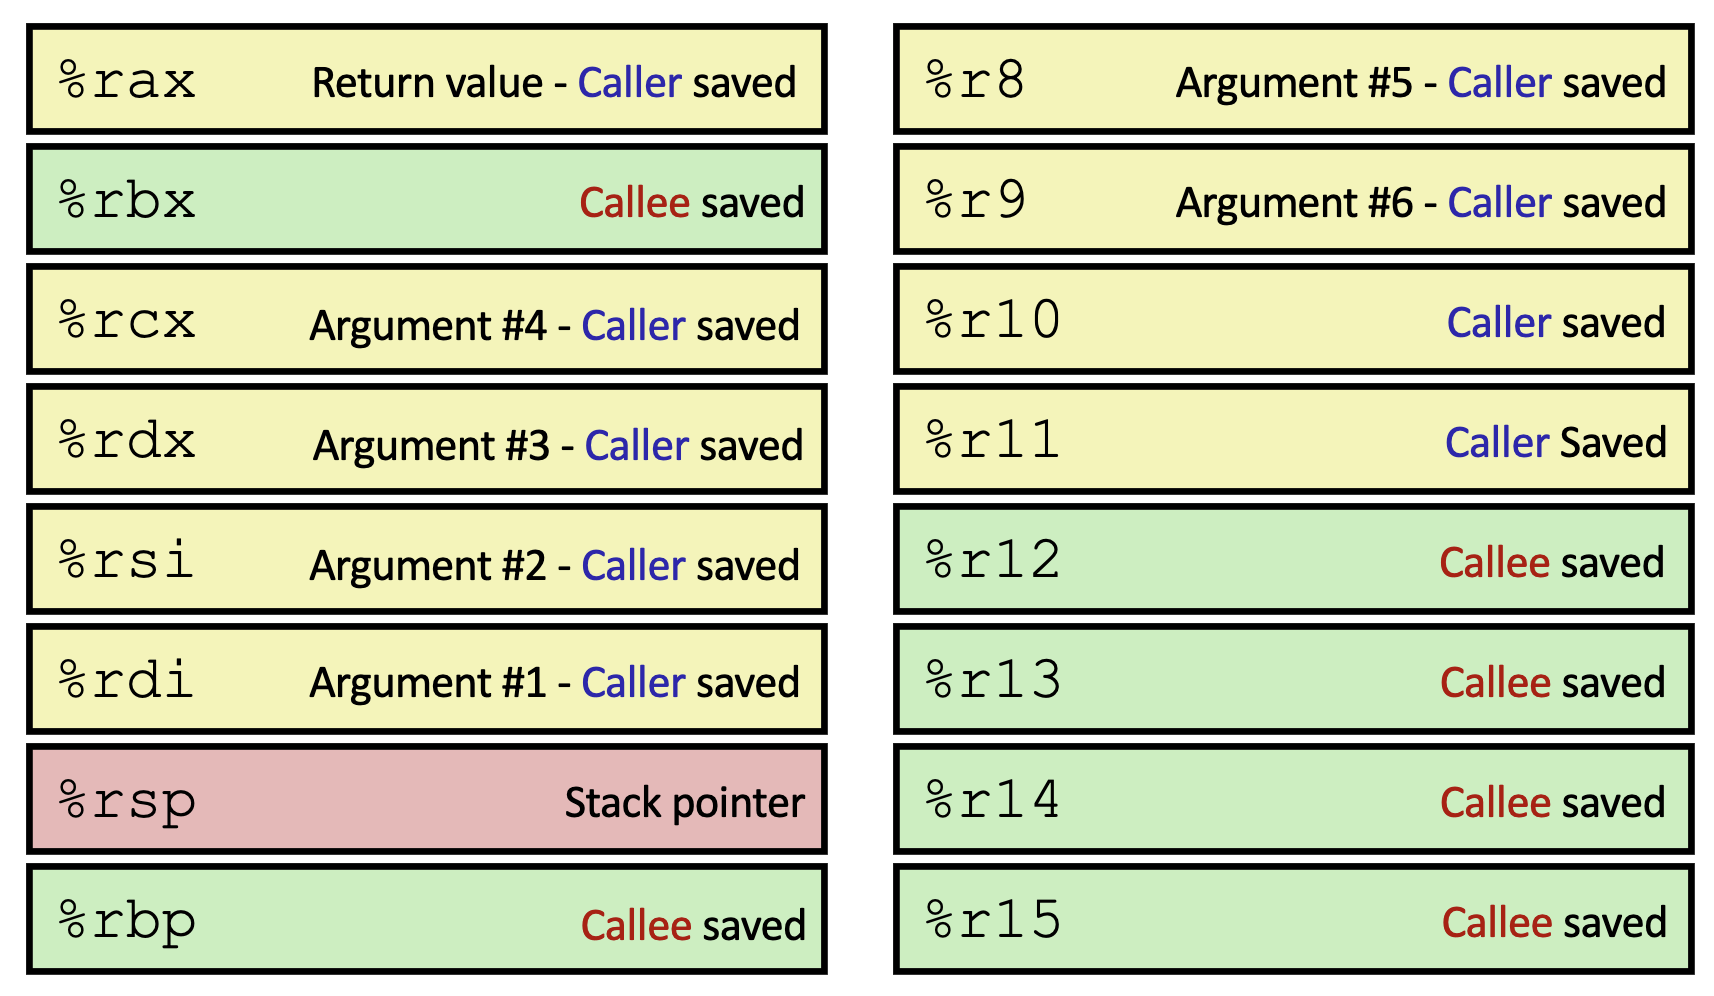
\includegraphics[scale=0.4]{img/caller_callee_save.png}
    \caption{Caller save and callee save registers. } 
    \label{fig:caller_callee_save}
  \end{figure}

  So far, we've traced through simple functions in assembly. In this section, we discuss the interaction between multiple functions in assembly in the context of a larger program. We also introduce some new instructions involved with function management. 

  \begin{definition}[Leave]
    The \textbf{leave} instruction is used to deallocate the current stack frame. For example, the leaveq instruction is a shorthand that the compiler uses to restore the stack and frame pointers as it prepares to leave a function. When the callee function finishes execution, leaveq ensures that the frame pointer is restored to its previous value. It is equivalent to the following two instructions: 
    \begin{align*}
      \texttt{leaveq} && \texttt{movq \%rbp, \%rsp} \\
                      && \texttt{popq \%rbp}
    \end{align*}
  \end{definition}

  \begin{definition}[Call and Return]
    The \textbf{call} instruction is used to call a function and the \textbf{ret} to return from a function. The callq and retq instructions play a prominent role in the process where one function calls another. Both instructions modify the instruction pointer (register \%rip). 

    \begin{enumerate}
      \item When the caller function executes the callq instruction, the current value of \%rip is saved on the stack to represent the return address, or the program address at which the caller resumes executing once the callee function finishes. The callq instruction also replaces the value of \%rip with the address of the callee function. 
        \begin{align*}
          \texttt{callq addr <fname>} && \texttt{push \%rip} \\
                                      && \texttt{mov addr, \%rip}
        \end{align*}
      \item The retq instruction restores the value of \%rip to the value saved on the stack, ensuring that the program resumes execution at the program address specified in the caller function. Any value returned by the callee is stored in \%rax or one of its component registers (e.g., \%eax). The retq instruction is usually the last instruction that executes in any function.
        \begin{align*}
          \texttt{retq} && \texttt{pop \%rip} \\
        \end{align*}
    \end{enumerate}
  \end{definition}

  Let's work through an example to solidify our knowledge. 

  \begin{example}[Calling Functions in Assembly]
    Let's take the following code and trace through main. 
    \begin{figure}[H]
      \centering 
      \noindent\begin{minipage}{.25\textwidth}
      \begin{lstlisting}[]{Code}
        #include <stdio.h>

        int assign(void) {
            int y = 40;
            return y;
        }

        int adder(void) {
            int a;
            return a + 2;
        }

        int main(void) {
            int x;
            assign();
            x = adder();
            printf("x is: %d\n", x);
            return 0;
        }
        .
        .
        .
        .
        .
        .
        .
        .
        .
        .
        .
        .
      \end{lstlisting}
      \end{minipage}
      \hfill
      \begin{minipage}{.74\textwidth}
      \begin{lstlisting}[]{Output}
        0000000000400526 <assign>:
          400526:       55                      push   %rbp
          400527:       48 89 e5                mov    %rsp,%rbp
          40052a:       c7 45 fc 28 00 00 00    movl   $0x28,-0x4(%rbp)
          400531:       8b 45 fc                mov    -0x4(%rbp),%eax
          400534:       5d                      pop    %rbp
          400535:       c3                      retq

        0000000000400536 <adder>:
          400536:       55                      push   %rbp
          400537:       48 89 e5                mov    %rsp,%rbp
          40053a:       8b 45 fc                mov    -0x4(%rbp),%eax
          40053d:       83 c0 02                add    $0x2,%eax
          400540:       5d                      pop    %rbp
          400541:       c3                      retq

        0000000000400542 <main>:
          400542:       55                      push   %rbp
          400543:       48 89 e5                mov    %rsp,%rbp
          400546:       48 83 ec 10             sub    $0x10,%rsp
          40054a:       e8 e3 ff ff ff          callq  400526 <assign>
          40054f:       e8 d2 ff ff ff          callq  400536 <adder>
          400554:       89 45 fc                mov    %eax,-0x4(%rbp)
          400557:       8b 45 fc                mov    -0x4(%rbp),%eax
          40055a:       89 c6                   mov    %eax,%esi
          40055c:       bf 04 06 40 00          mov    $0x400604,%edi
          400561:       b8 00 00 00 00          mov    $0x0,%eax
          400566:       e8 95 fe ff ff          callq  400400 <printf@plt>
          40056b:       b8 00 00 00 00          mov    $0x0,%eax
          400570:       c9                      leaveq
          400571:       c3                      retq
      \end{lstlisting}
      \end{minipage}
      \caption{C code and its assembly equivalent. Main function calls two other functions. } 
      \label{fig:calling_functions}
    \end{figure}

    Let's trace through what happens here in detail. This will be long. 

    \begin{enumerate}
      \item \texttt{\%rbp} is the base pointer that is initialized to something. Before we even begin main, say that we have the following initializations, where \texttt{\%eax}, \texttt{\%edi} is garbage. \texttt{\%rsp} denotes where on the stack we are right before calling to main, \textbf{\%rbp} is the base pointer to the current program, and \textbf{\%rip} should be the address of the first instruction in main. Again since we work with integers we use the lower 32-bits of the registers. \texttt{\%rip} now points to the next instruction. 
        \begin{center}
          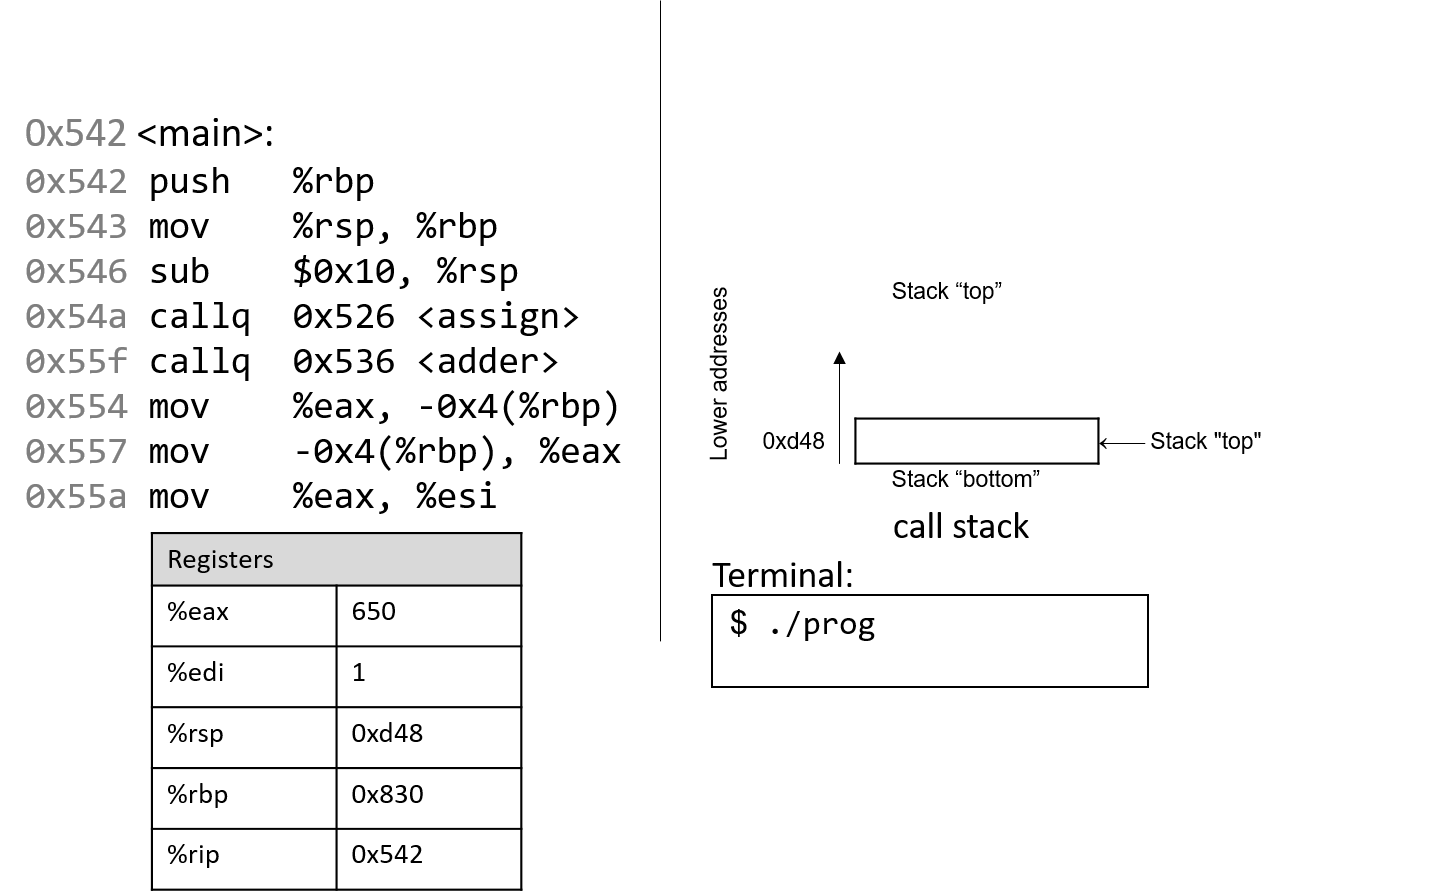
\includegraphics[scale=0.5]{img/Slide1.png}
        \end{center}  

      \item Now we start the main function. By calling main, the base pointer \texttt{\%rbp} of the stack outside of the main frame will be overwritten by the base of the main stack frame, so we must save it for when main is done. Therefore, we push it onto the stack where \texttt{\%rsp} is pointing. \texttt{\%rip} now points to the next instruction. 
        \begin{center}
          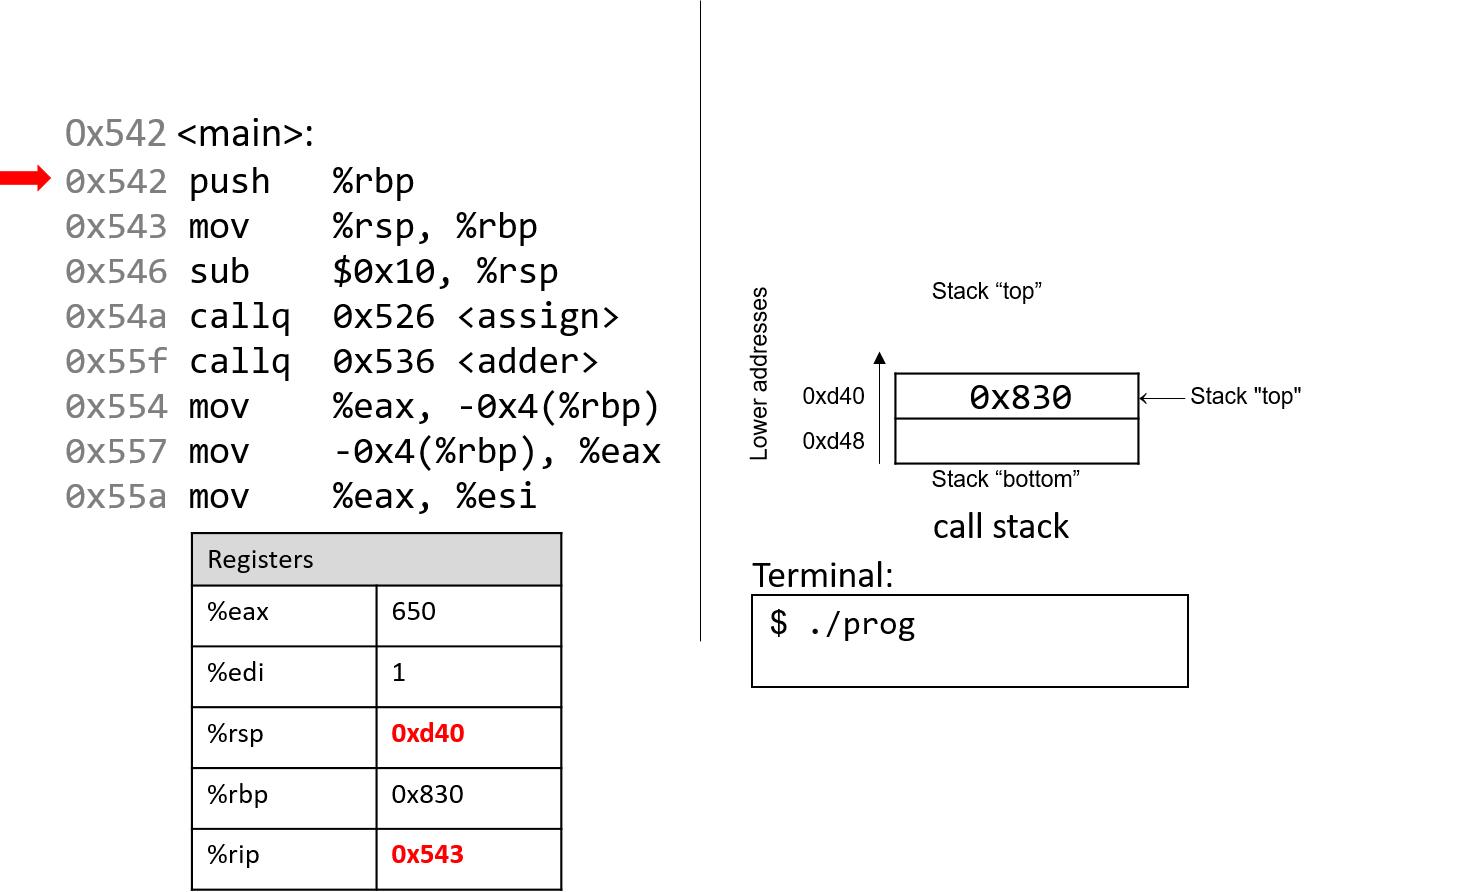
\includegraphics[scale=0.5]{img/Slide2.png}
        \end{center}

      \item Then we actually change the location of the base pointer to the top of the stack, which now includes the first instruction in main. 
        \begin{center}
          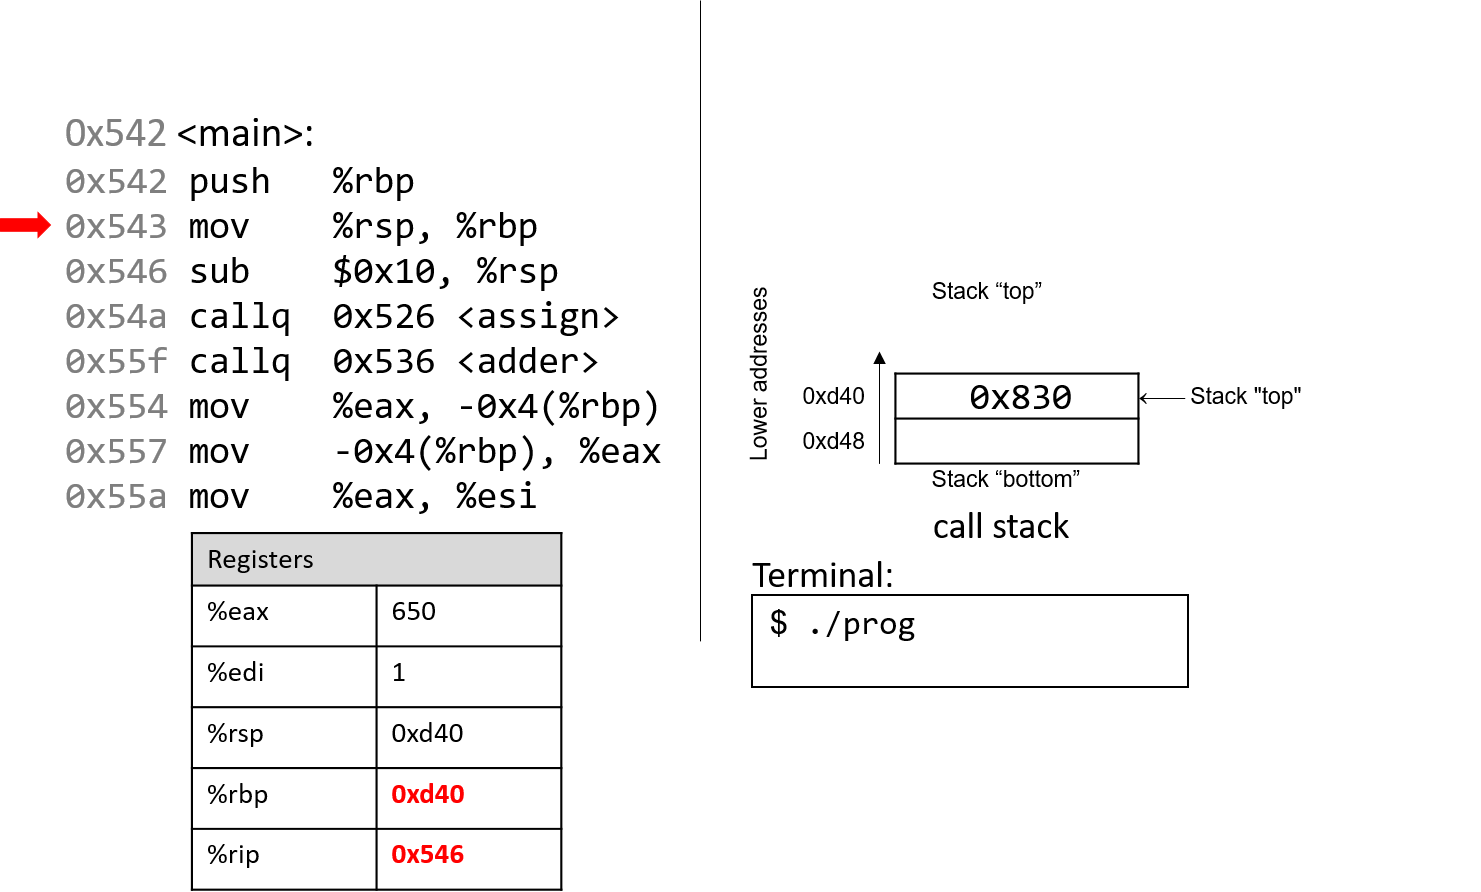
\includegraphics[scale=0.5]{img/Slide3.png}
        \end{center} 

      \item Now we manually change the stack pointer and have it grow by two bytes (\texttt{0x10}). Therefore, \texttt{\%rsp} is decremented by \texttt{0x10} and \texttt{\%rip} points to the next instruction at \texttt{0x54a}. 
        \begin{center}
          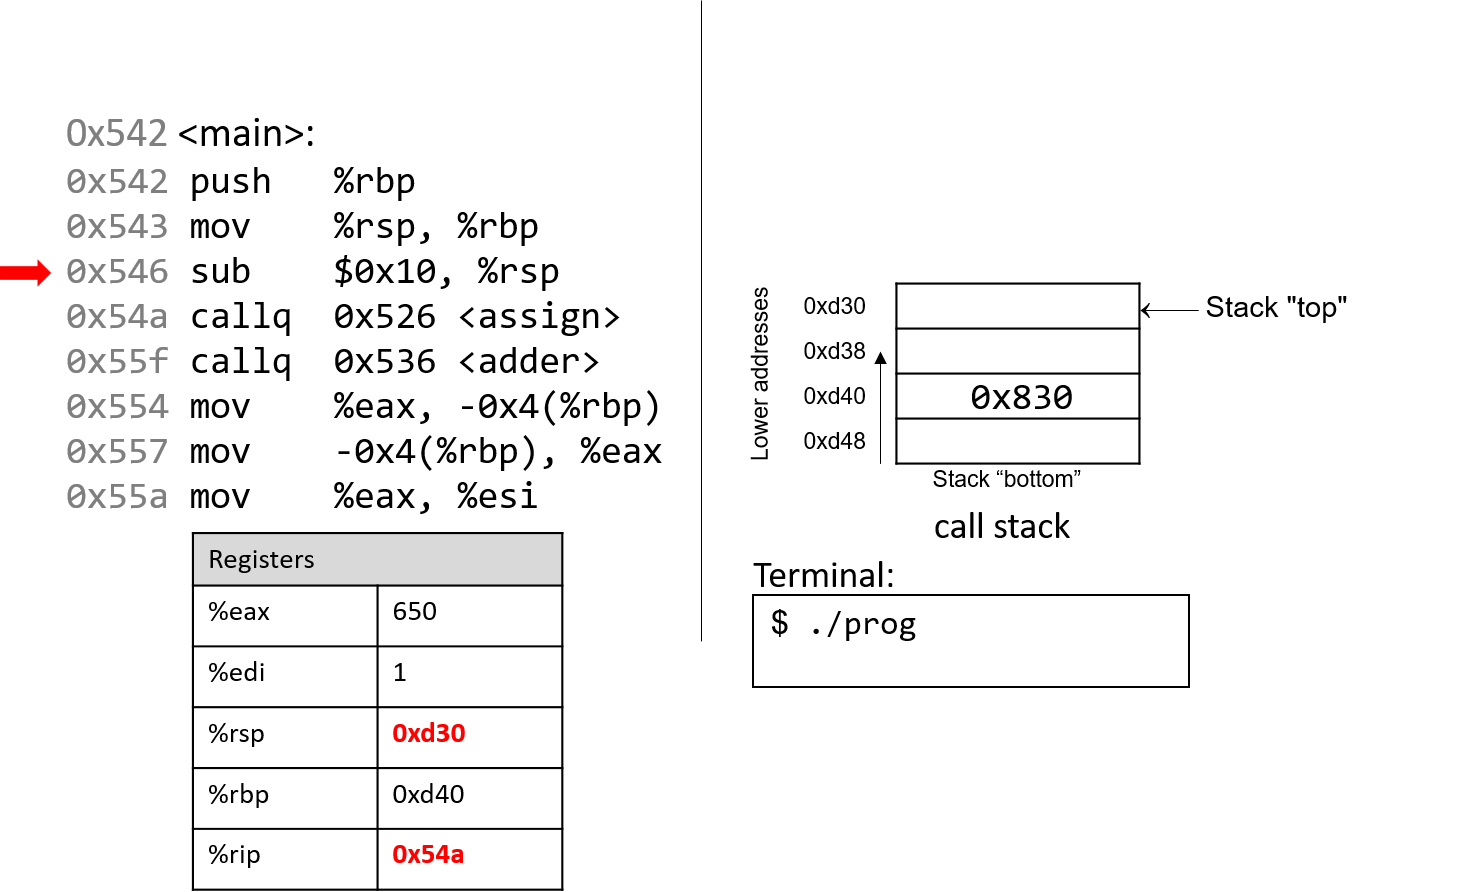
\includegraphics[scale=0.5]{img/Slide4.png}
        \end{center}
        
      \item Now the next instruction pointed at by \texttt{\%rip} is the \texttt{callq} instruction, which tells to go to the address of the \texttt{assign} function. We by default first update \texttt{\%rip} to point to the next instruction at \texttt{0x55f}. However, this should not be the actual next instruction that we execute since we are calling another function. Rather, we want to update \texttt{\%rip} to address \texttt{0x526} where \texttt{assign} is located at, but after completion we also want to know that we want to execute the instruction after it at address \texttt{0x55f}. Therefore, we should \textit{save} address \texttt{0x55f} onto the stack and then update \texttt{\%rip} to point to \texttt{0x526}. This is what we refer to as a \textbf{return address}. 
        \begin{center}
          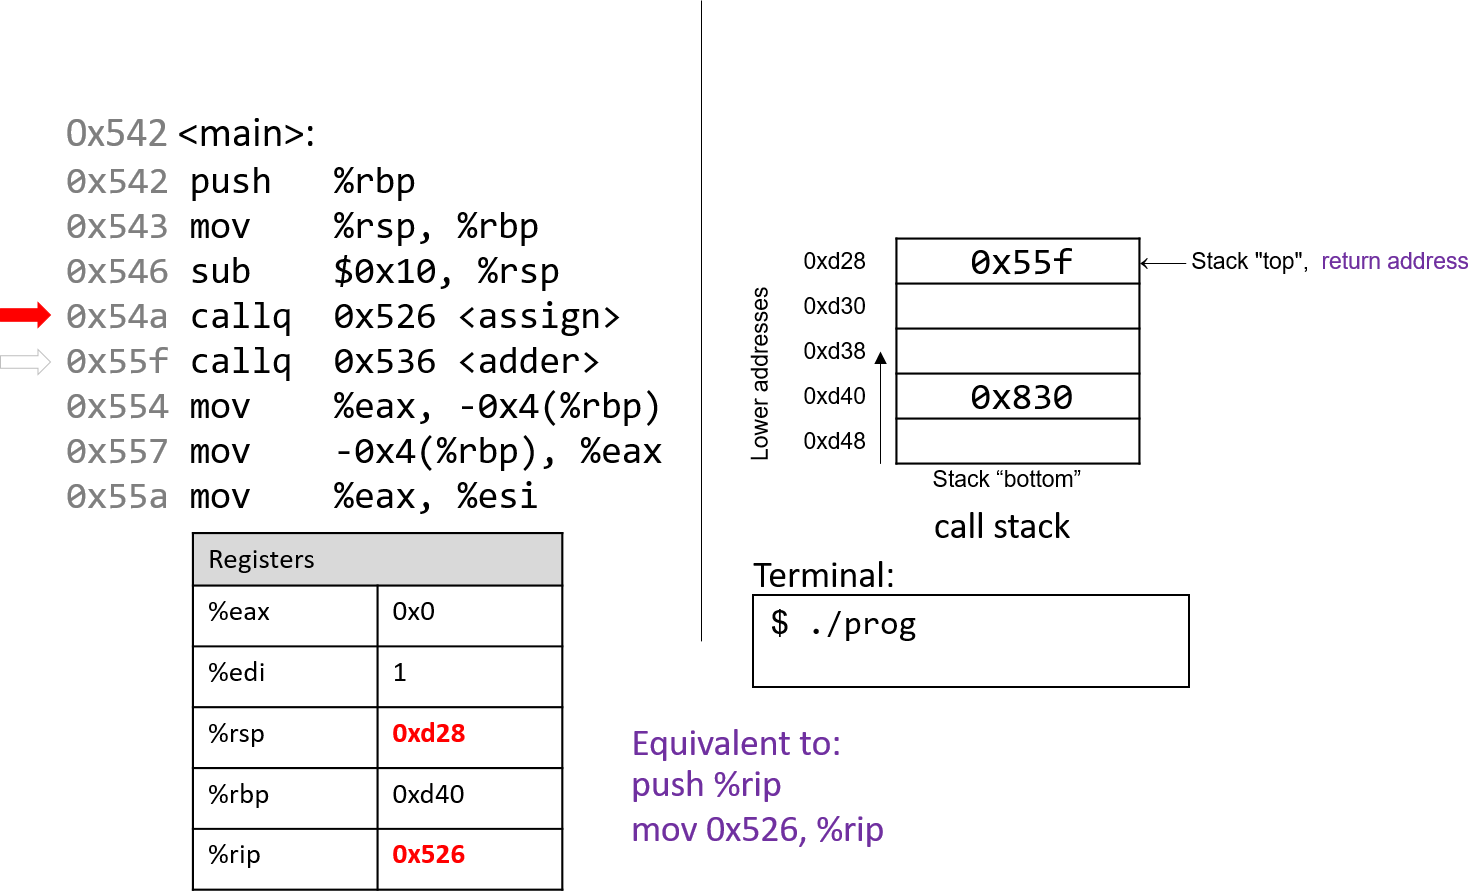
\includegraphics[scale=0.5]{img/Slide5.png}
        \end{center}

      \item \texttt{\%rip} is incremented to the next address. We step into the \texttt{assign} function, which is now a new stack frame, so the first thing we do is save the base pointer of the main stack frame onto the stack since we must immediately update it with the base pointer of the assign stack frame, which is where \texttt{\%rsp} is pointing to. 
        \begin{center}
          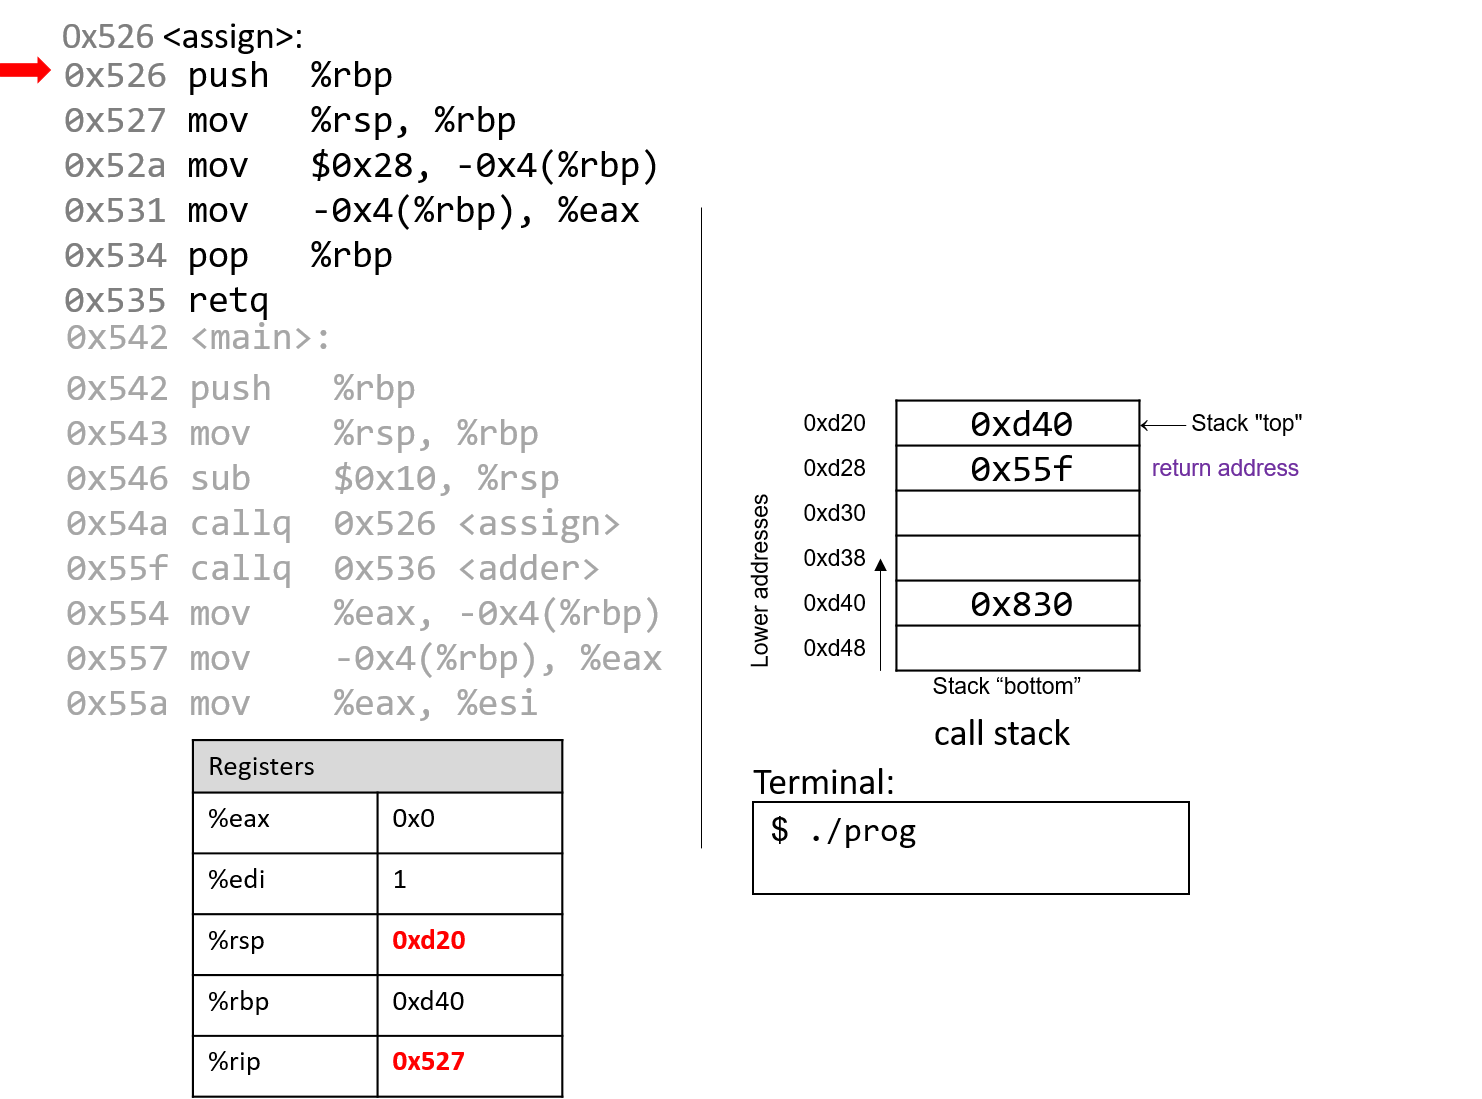
\includegraphics[scale=0.5]{img/Slide6.png}
        \end{center}

      \item \texttt{\%rip} is incremented to the next address. We then update the base pointer to the top of the stack. 
        \begin{center}
          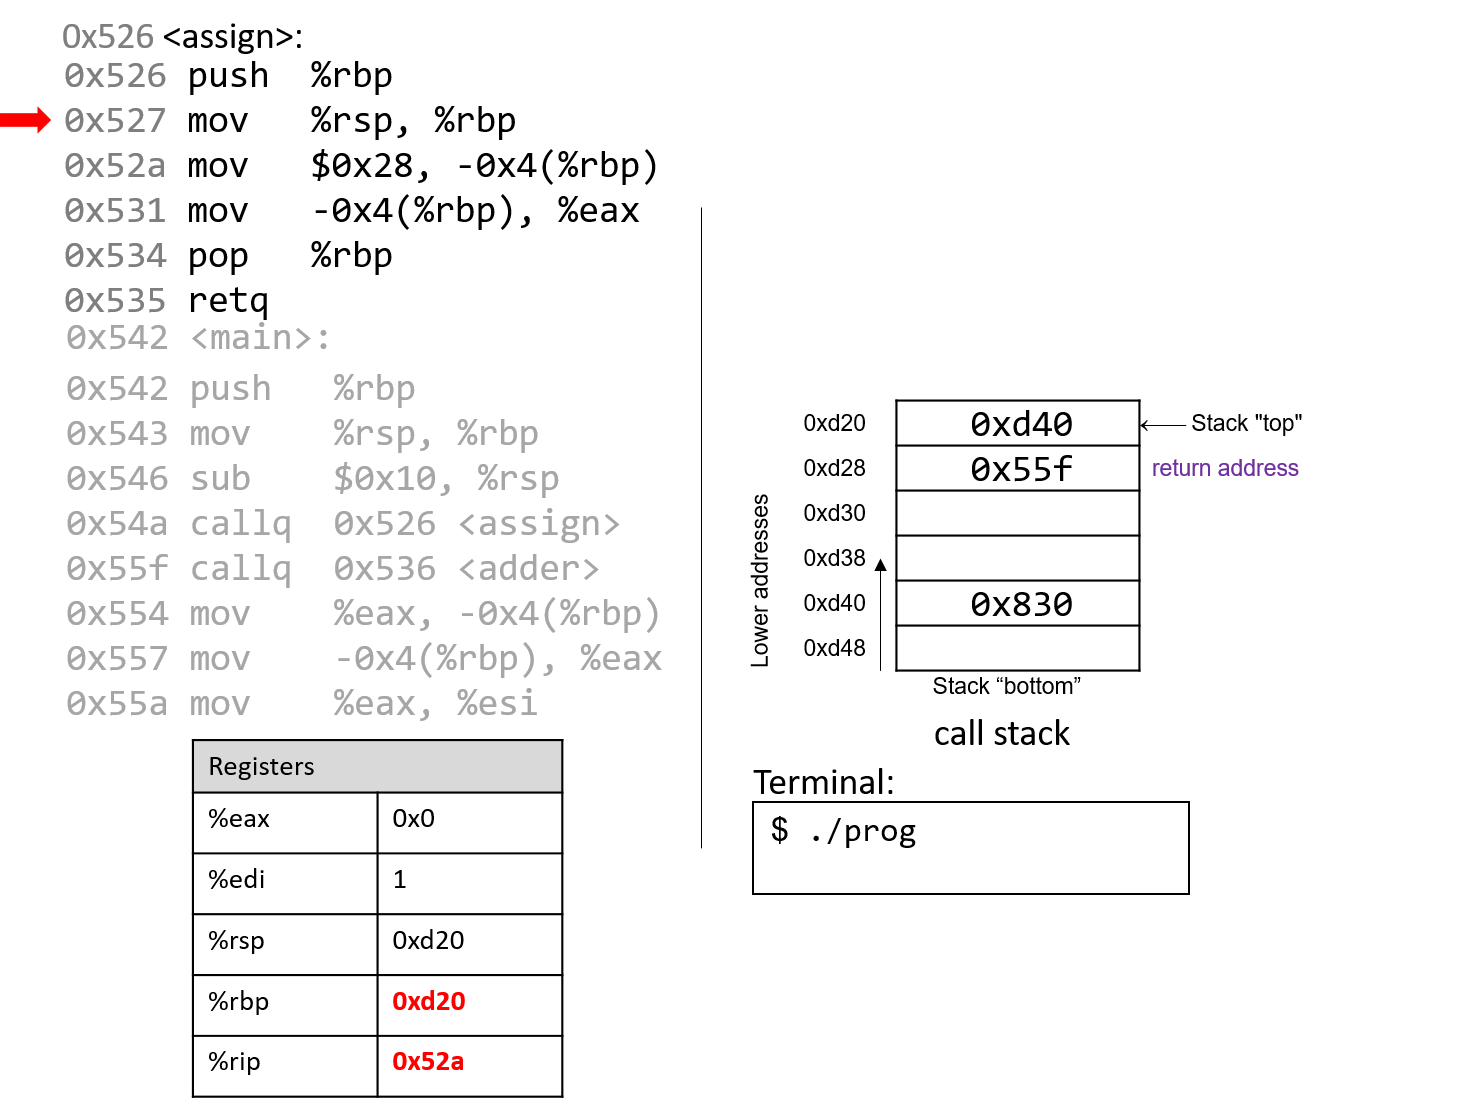
\includegraphics[scale=0.5]{img/Slide7.png}
        \end{center}

      \item Now we want to move the number \texttt{0x28} (40) into the memory location \texttt{-0x4(\%rbp)} of the stack, which is 4 bytes above the frame pointer, which is also the stack pointer. It is common that the frame pointer is used to reference locations on the stack. Note that this does not update the stack pointer.  
        \begin{center}
          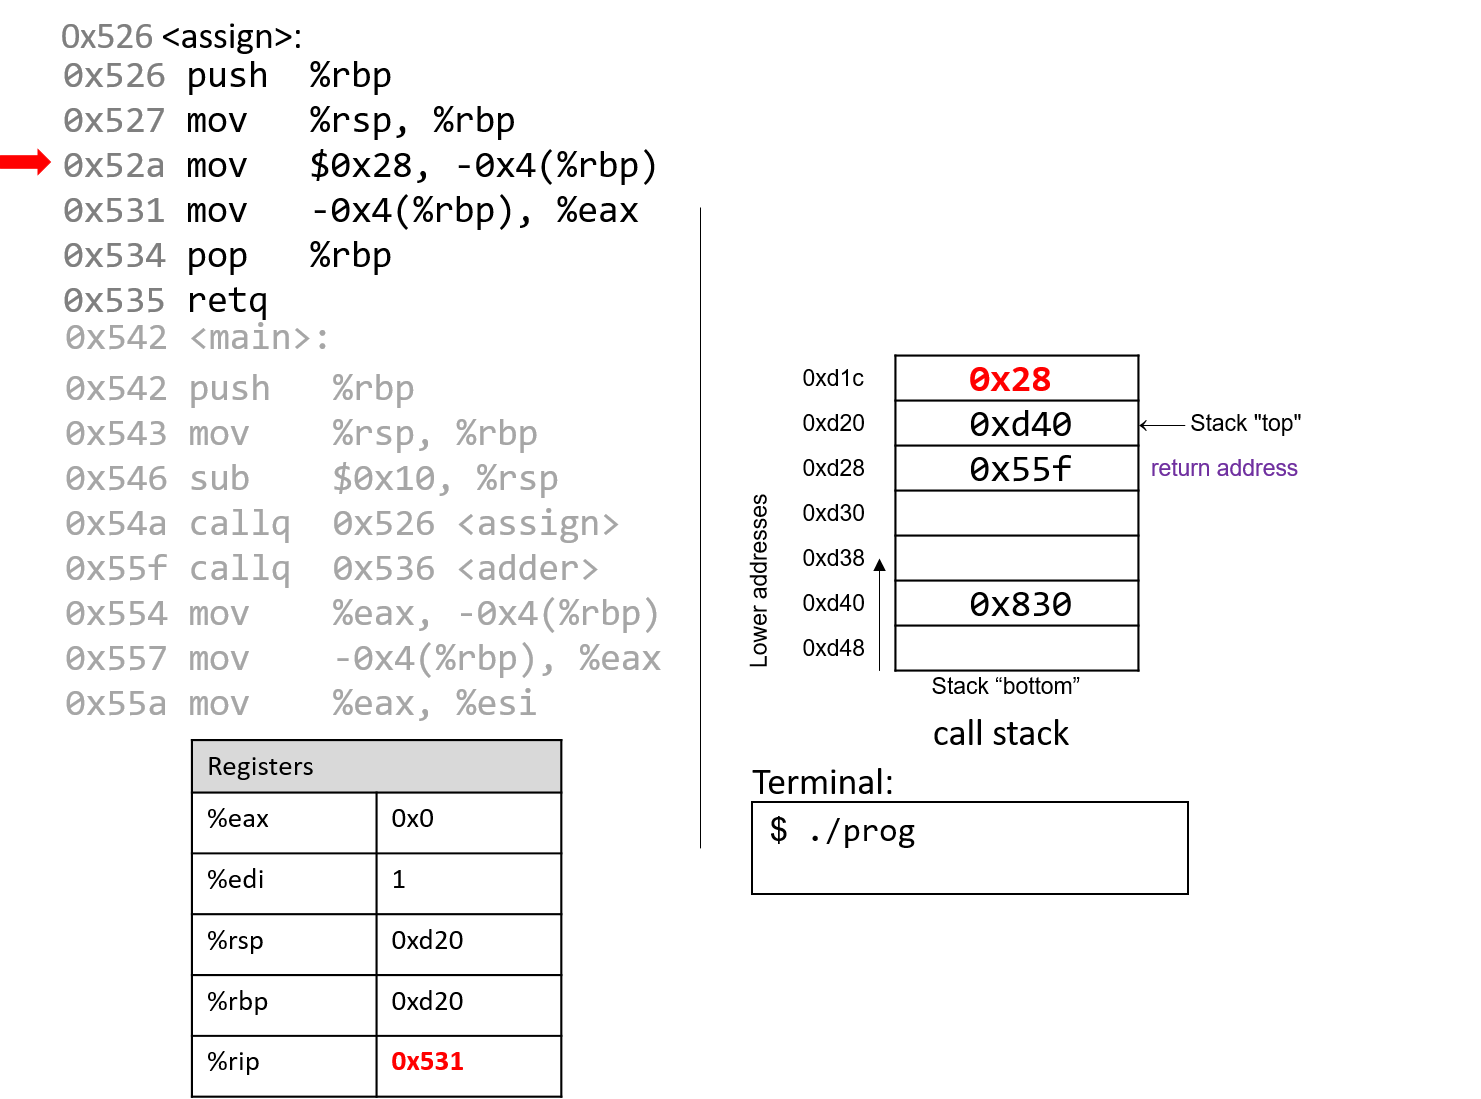
\includegraphics[scale=0.5]{img/Slide8.png}
        \end{center}

      \item Now we take the same address where we stored \texttt{0x28} to and move it into \texttt{\%eax}, effectively loading 40 onto the return value. 
        \begin{center}
          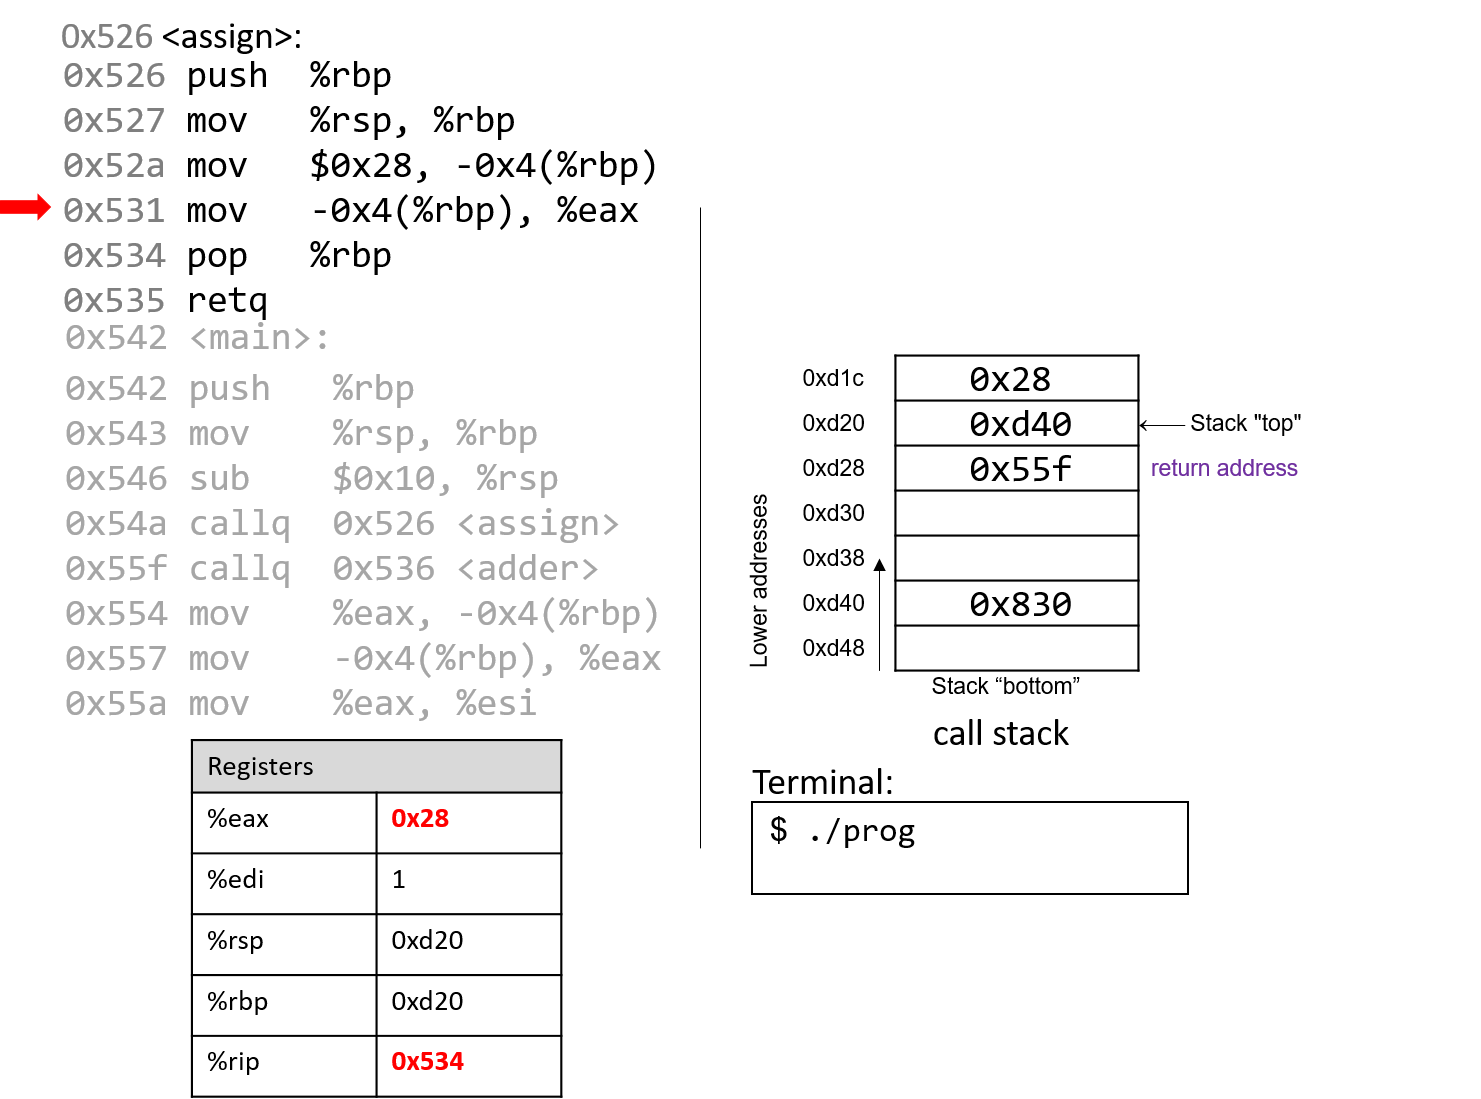
\includegraphics[scale=0.5]{img/Slide9.png}
        \end{center}

      \item We see that we will return this value soon, but before we do, we want to make sure that when the assign stack frame gets deleted (not really, but overwritten), we want to restore the base pointer of the main stack frame. We have already saved this before at \texttt{\%rsp}, which hasn't changed since we only worked with displacements from the base pointer. We retrieve the main stack pointer data and load it back into \texttt{\%rbp}. Note that this increments \texttt{\%rsp} by 8 bytes, shrinking the stack, and we are technically out of the assign stack frame. 
        \begin{center}
          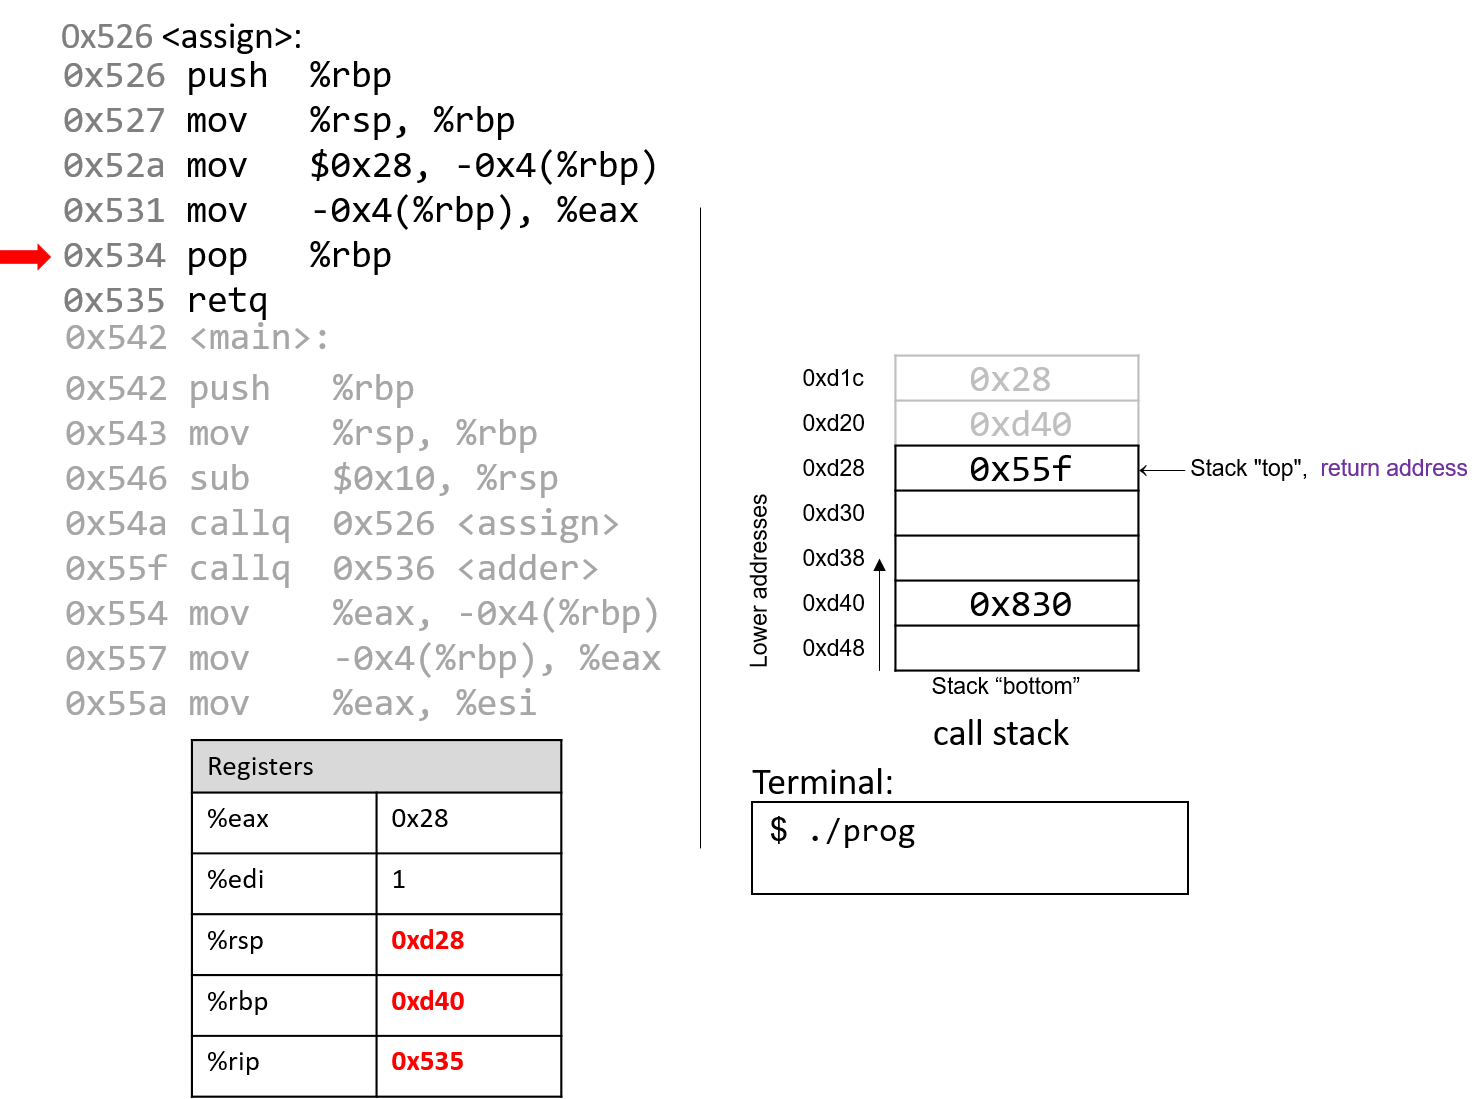
\includegraphics[scale=0.5]{img/Slide10.png}
        \end{center} 

      \item Note that at this point, since \texttt{\%rbp} was popped off, the next value that is at the top of the stack is the address \texttt{\%rip} that we store earlier, which points to the next execution in main. When \texttt{retq} executes, this value at the top of the stack is popped into \texttt{\%rip}, allowing main to continue executing within the main stack frame. Note that the return value is stored in \texttt{\%eax}.
        \begin{center}
          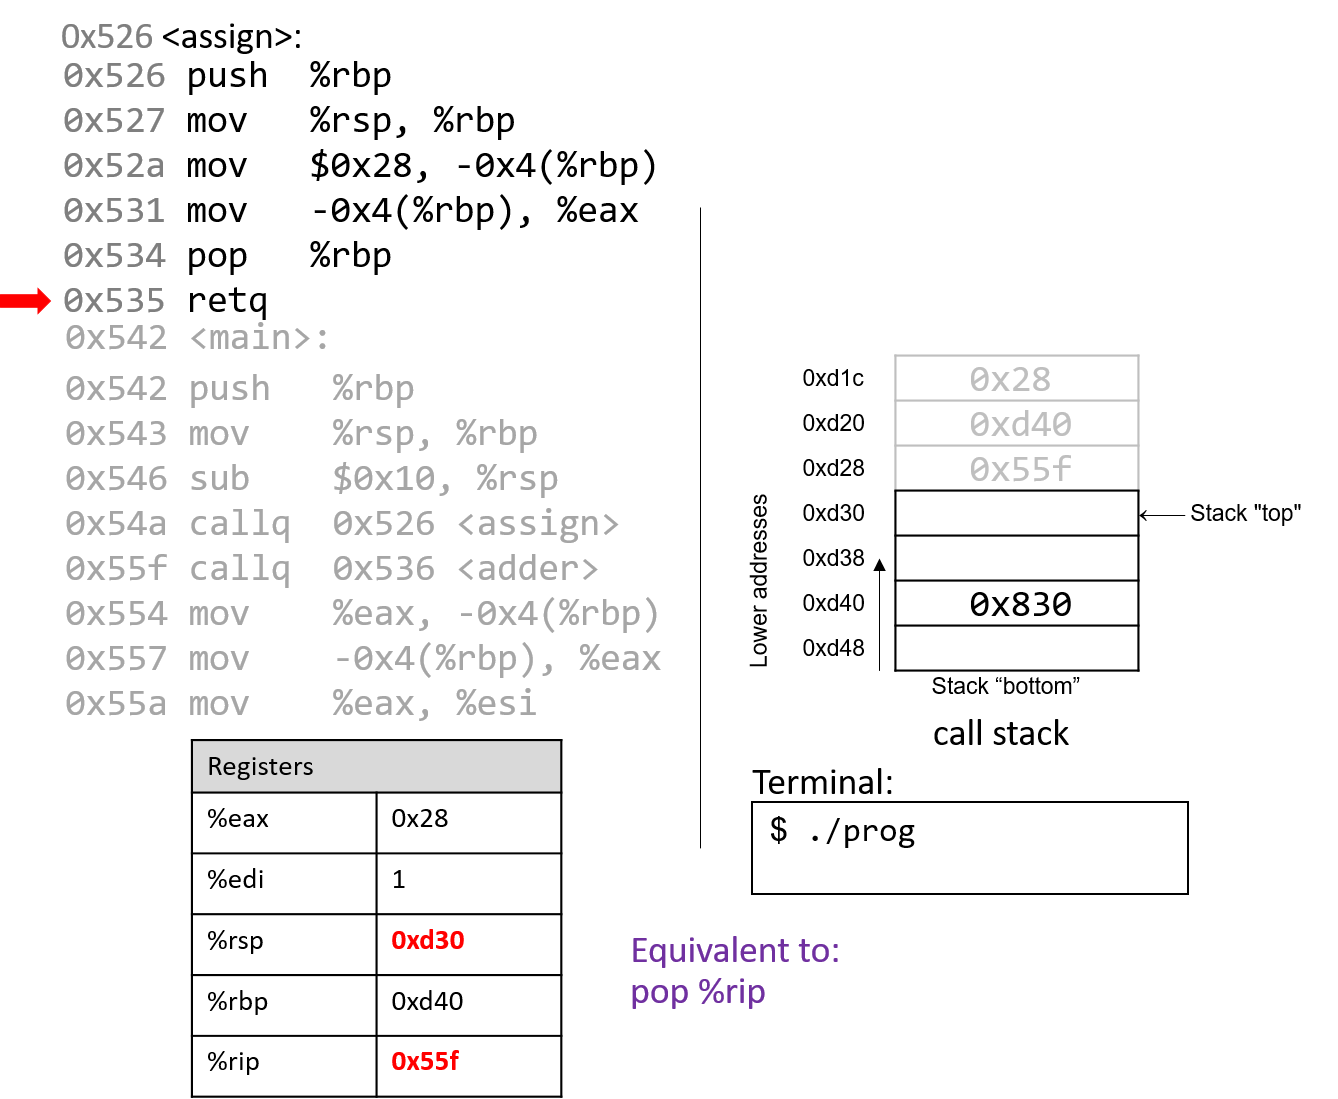
\includegraphics[scale=0.5]{img/Slide11.png}
        \end{center}

      \item Now we execute the next instruction in \texttt{\%rip} which is a call to the \texttt{adder} function. \texttt{\%rip} is automatically updated to the next address at \texttt{0x554}, but since this is a \texttt{callq} instruction, we first want to store this \texttt{\%rip} into the stack so we can come back to it, and then update \texttt{\%rip} to the first instruction in \texttt{adder}, which is address \texttt{0x536}. 
        \begin{center}
          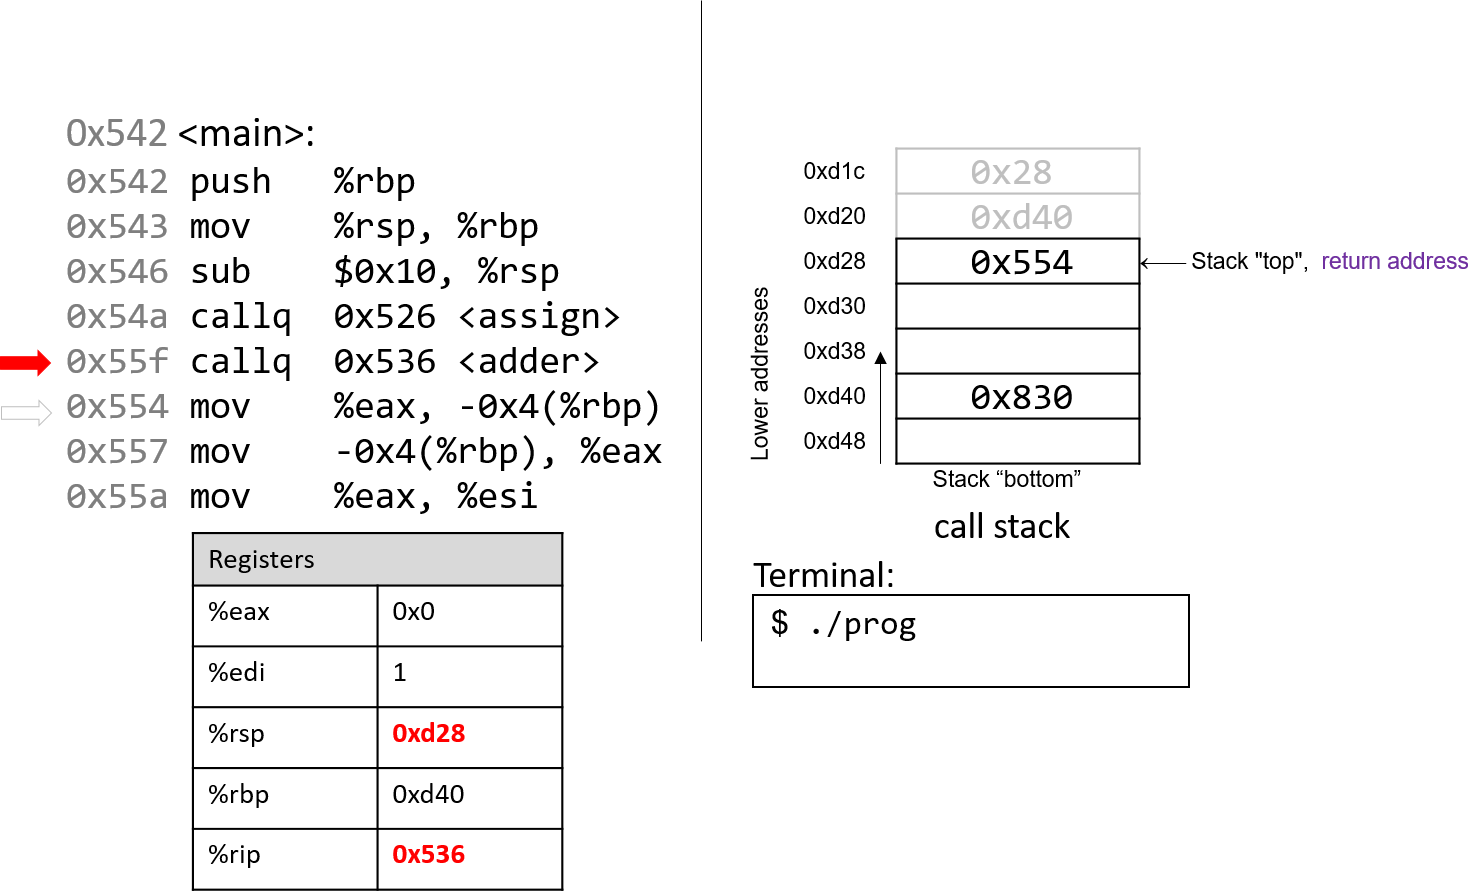
\includegraphics[scale=0.5]{img/Slide12.png}
        \end{center}

      \item Since we are in the adder function, this creates a new stack frame and we must update \texttt{\%rbp}. Again, we don't want to overwrite the base pointer of main, so we save it onto the stack by pushing \texttt{\%rbp}. 
        \begin{center}
          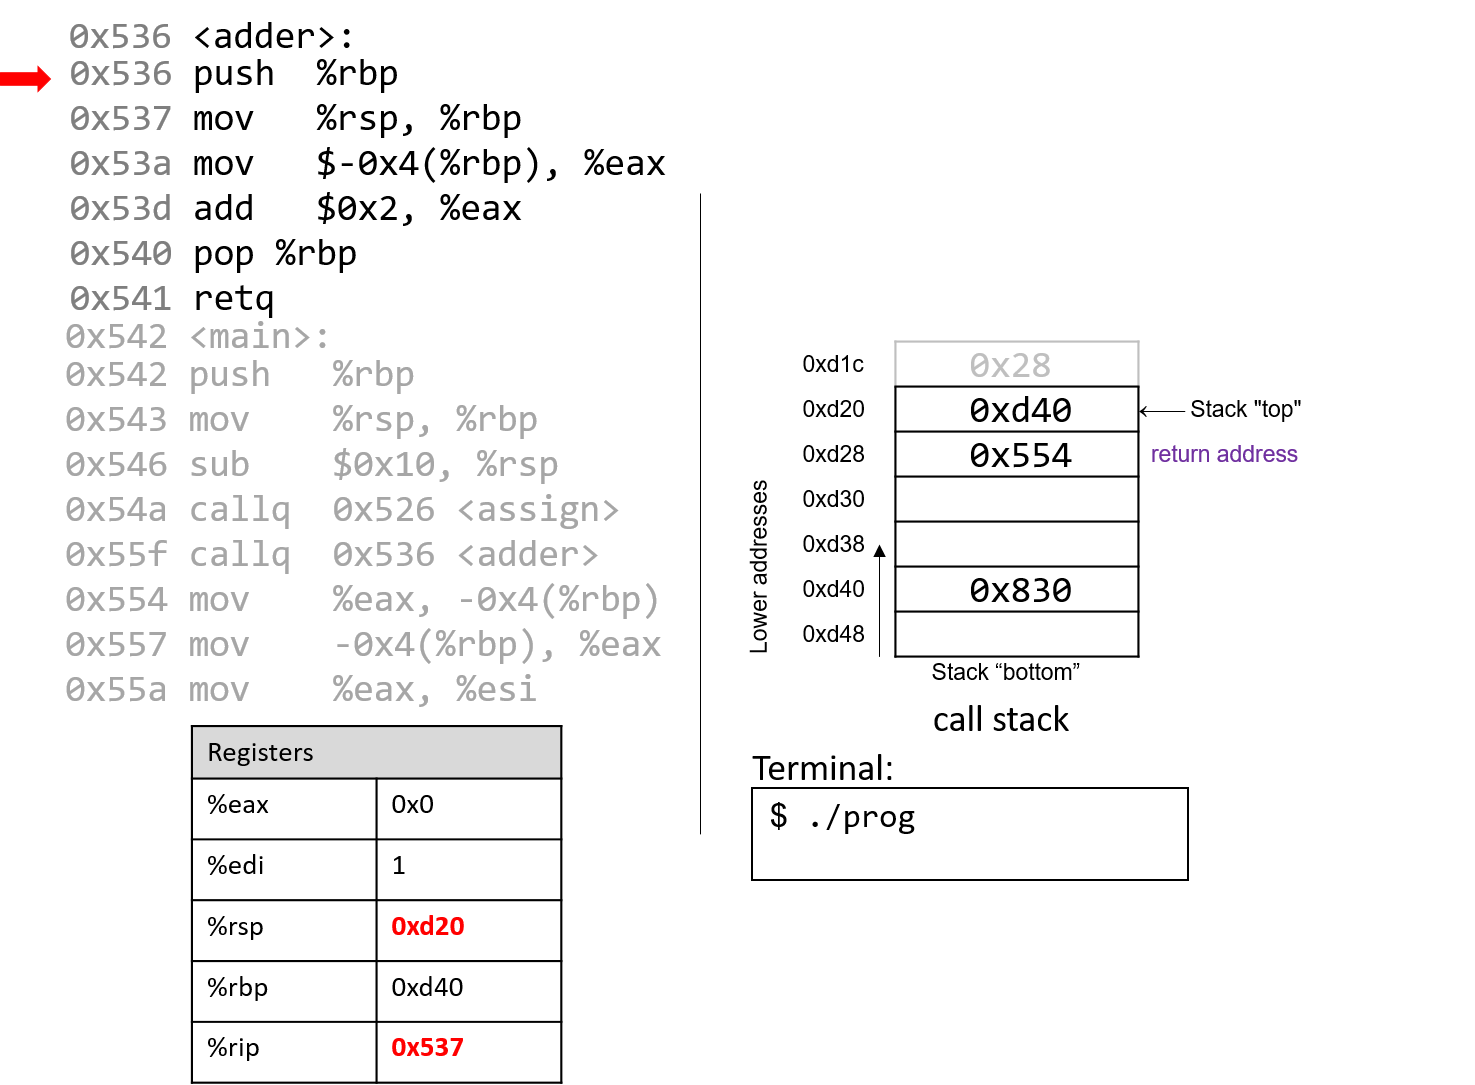
\includegraphics[scale=0.5]{img/Slide13.png}
        \end{center}

      \item Then we update \texttt{\%rbp} to the current stack pointer. 
        \begin{center}
          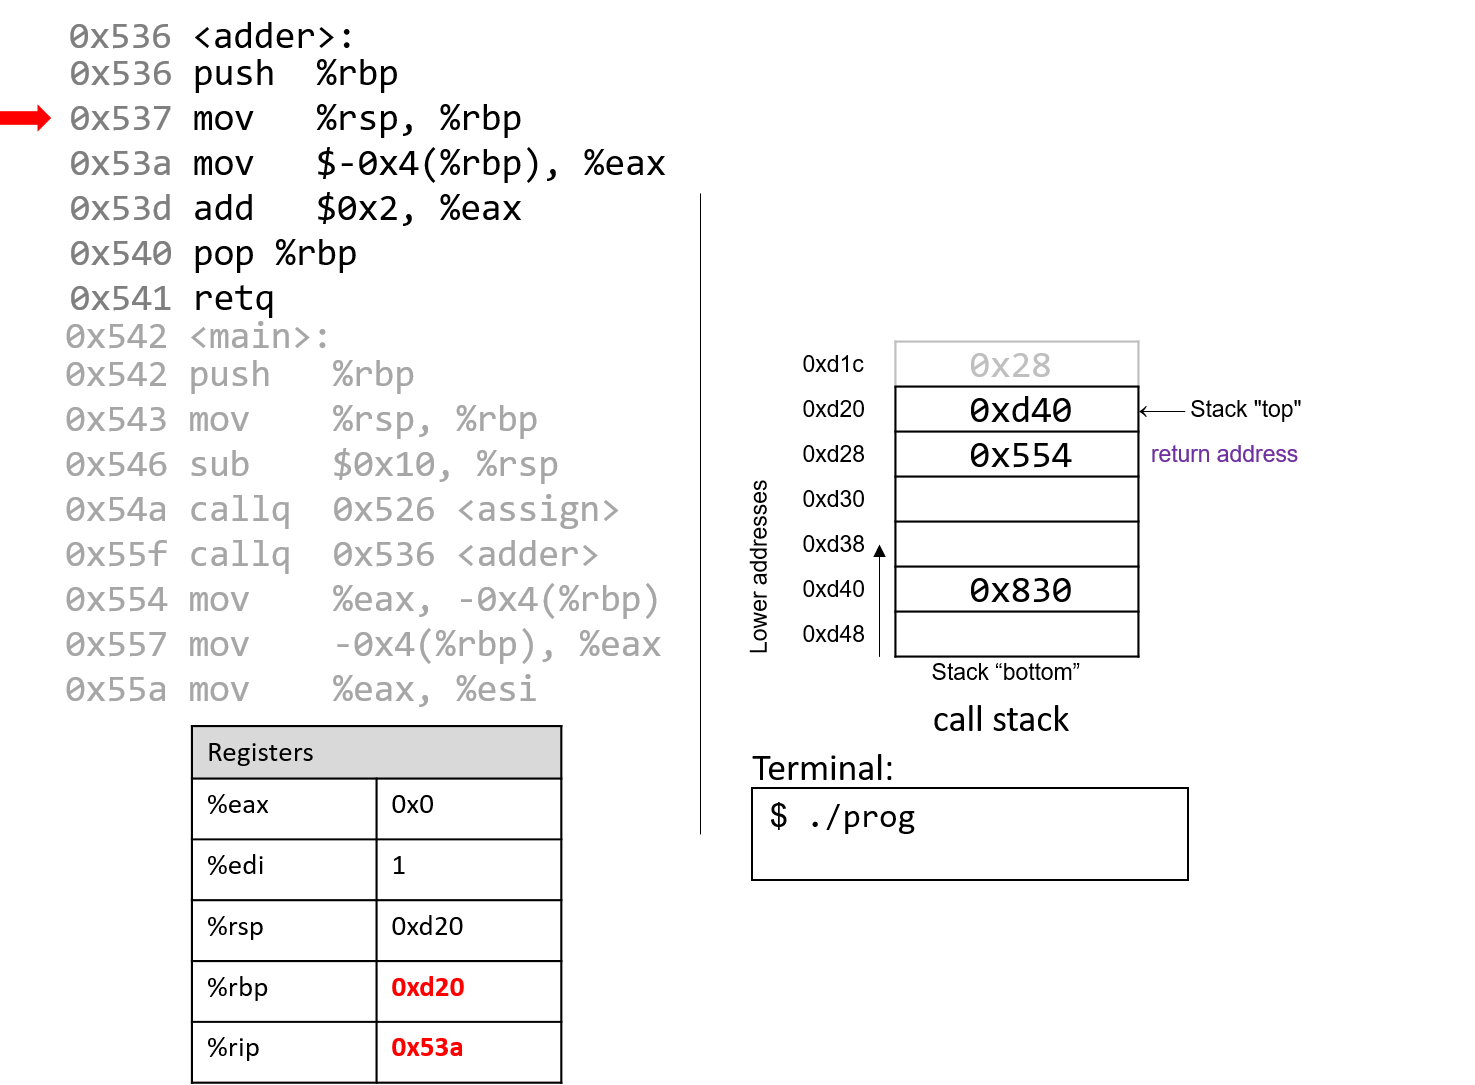
\includegraphics[scale=0.5]{img/Slide14.png}
        \end{center}

      \item This part is a bit tricky. Note that the value of \texttt{0x28} still lives at \texttt{0xd1c}, which is conveniently at address \texttt{-0x4(\%rbp)}. Therefore, when we call \texttt{int a;} in that corresponding line in \texttt{adder}, we can actually add 2 to it, though it seems like there was no value assigned to it. This is just a trick though. So, we can take these remnant value and store it into \texttt{\%eax}. 
        \begin{center}
          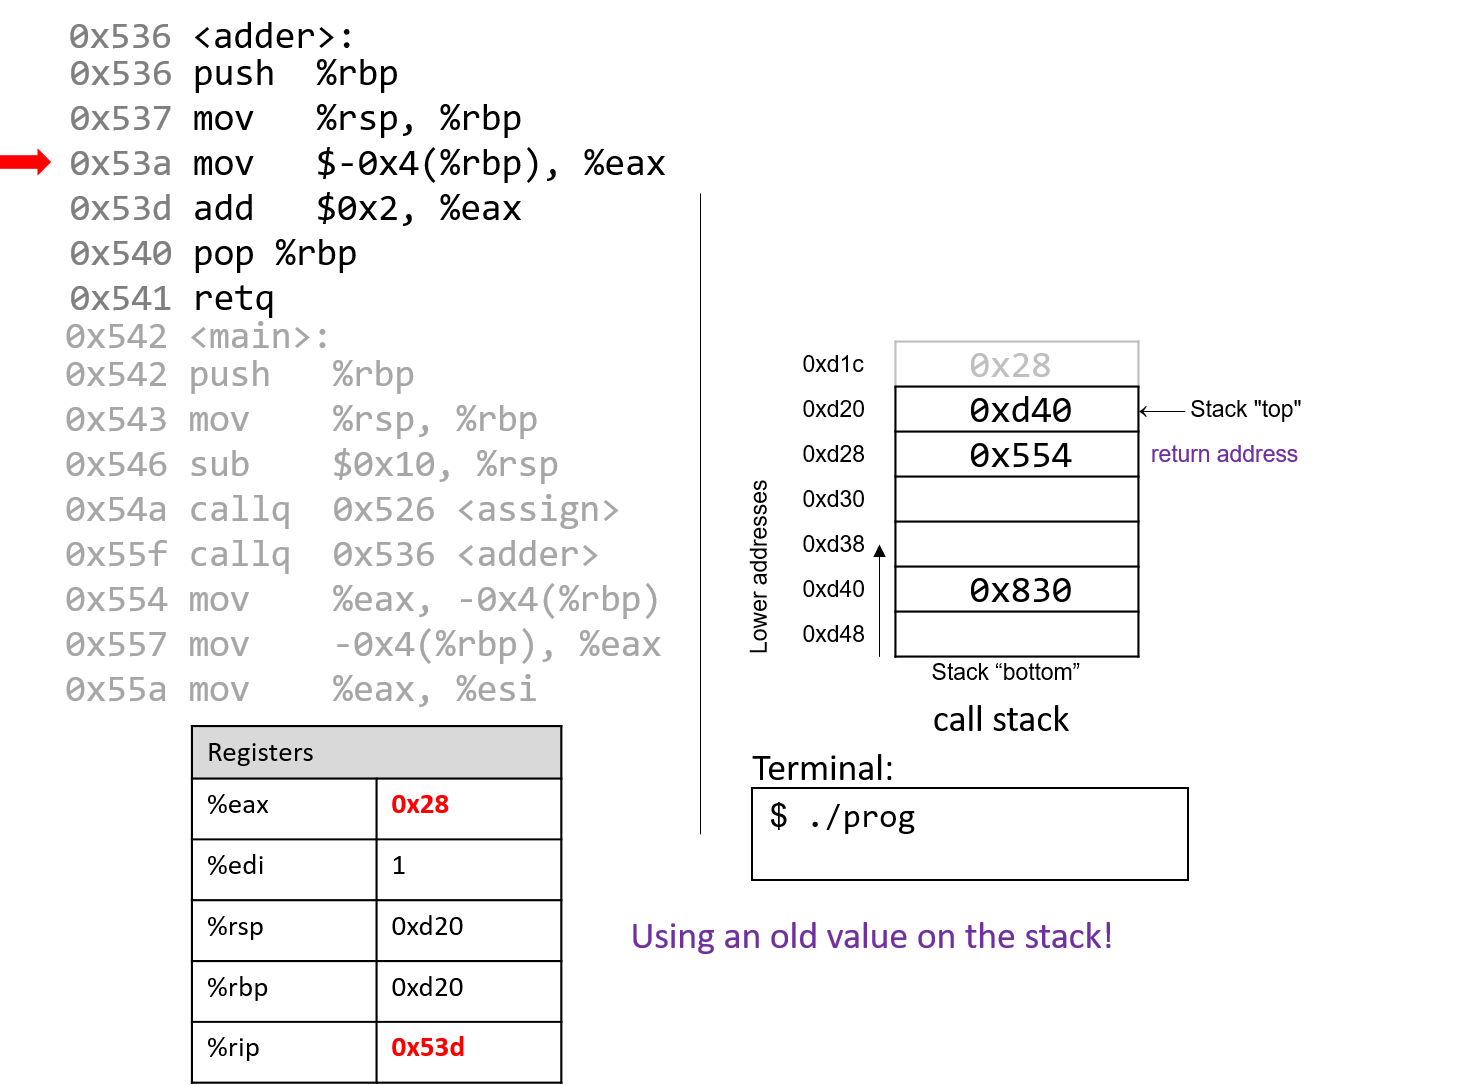
\includegraphics[scale=0.5]{img/Slide15.png}
        \end{center}

      \item We then add 2 to it. 
        \begin{center}
          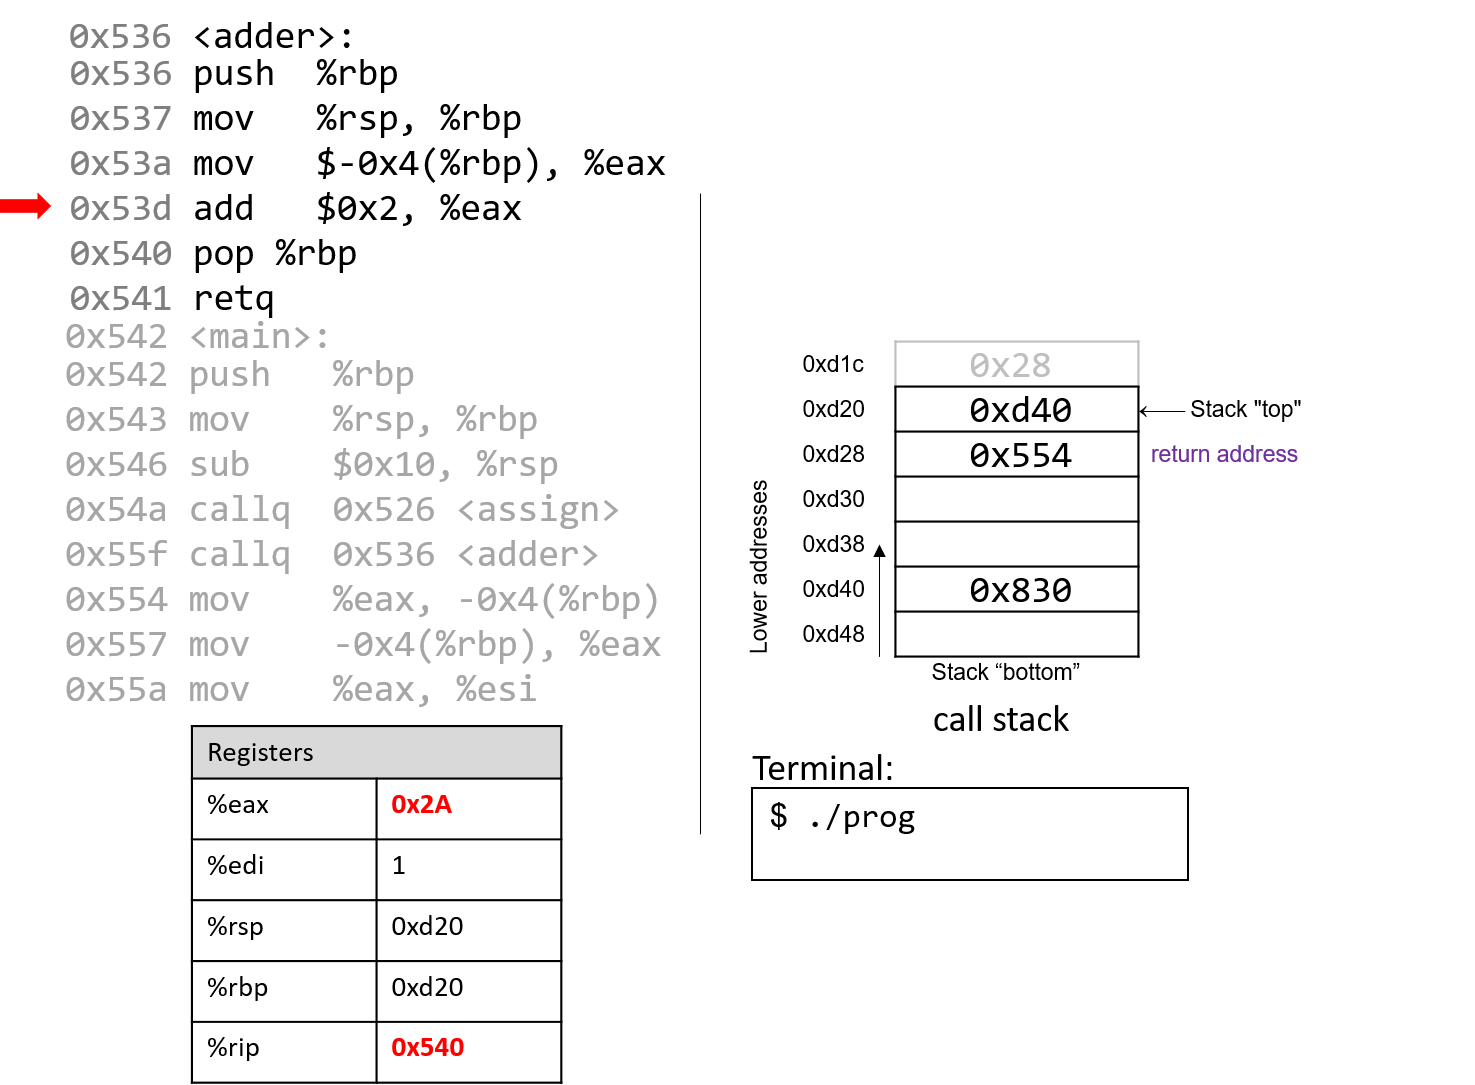
\includegraphics[scale=0.5]{img/Slide16.png}
        \end{center}

      \item Now we are almost done, so we pop the base pointer of the main stack frame, at \texttt{0xd40}, back into \texttt{\%rbp}. 
        \begin{center}
          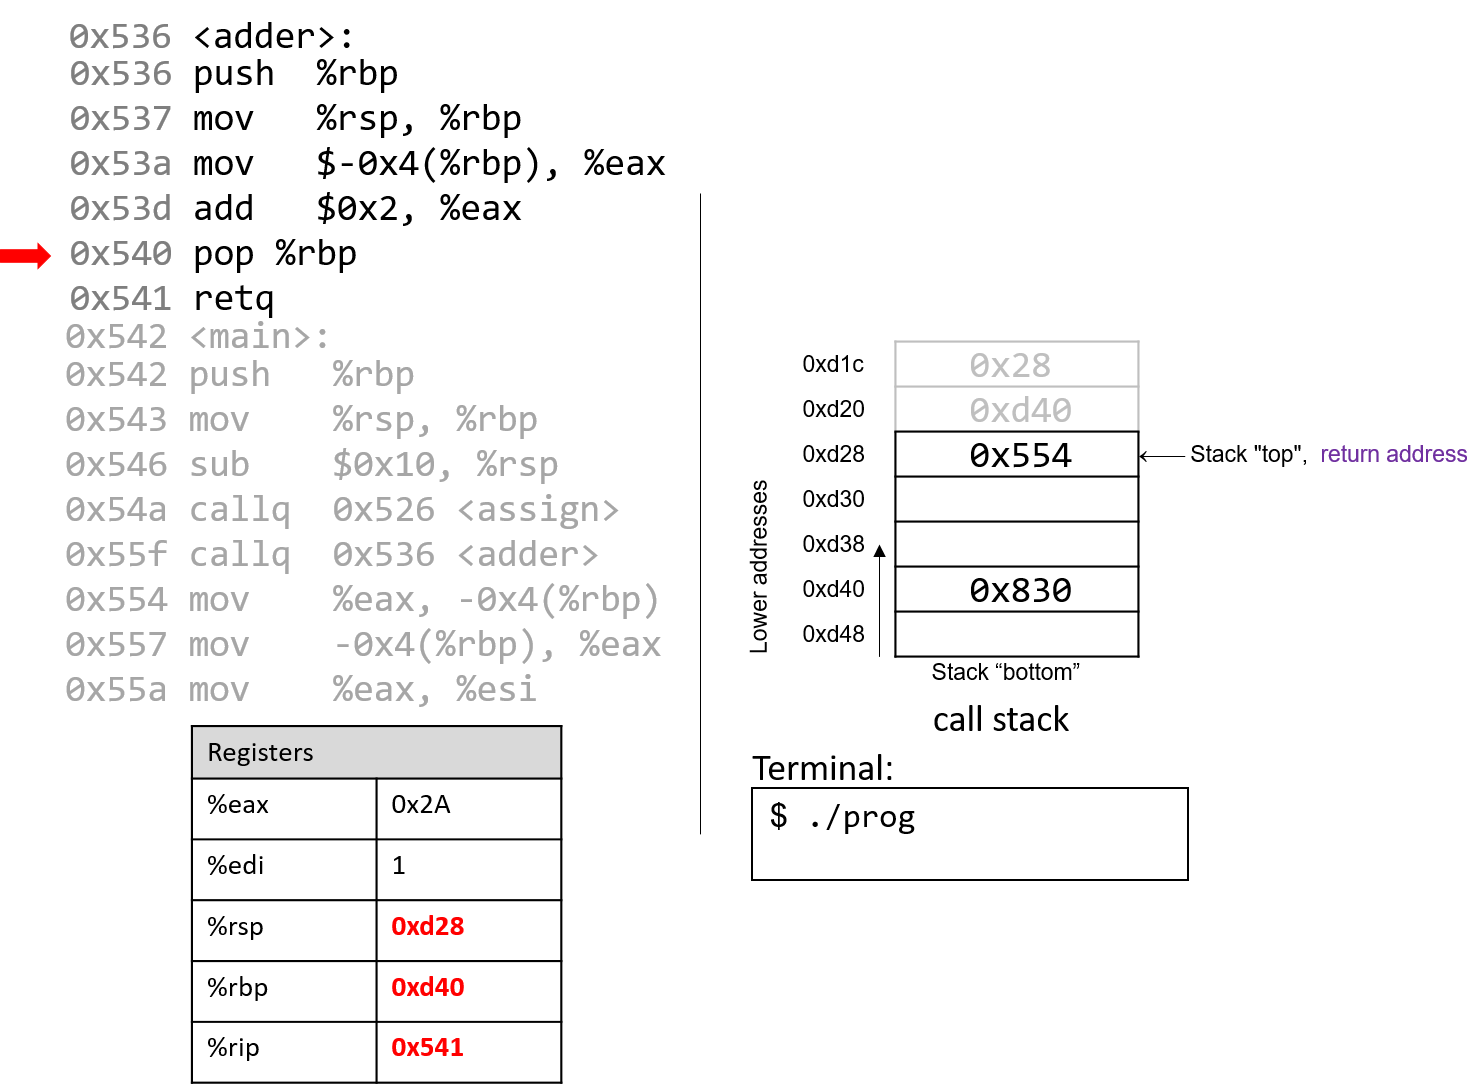
\includegraphics[scale=0.5]{img/Slide17.png}
        \end{center}

      \item We now return the value in \texttt{\%eax} and pop the base pointer of the adder stack frame, which simply updates the instruction pointer \texttt{\%rip} back to the next instruction in main. This is equivalent to \texttt{pop \%rip}, which is equivalent to moving the stack pointer \texttt{\%rsp} into \texttt{\%rip} and then shrinking the stack by 8 bytes \texttt{subq \$8, \%rsp}. 
        \begin{center}
          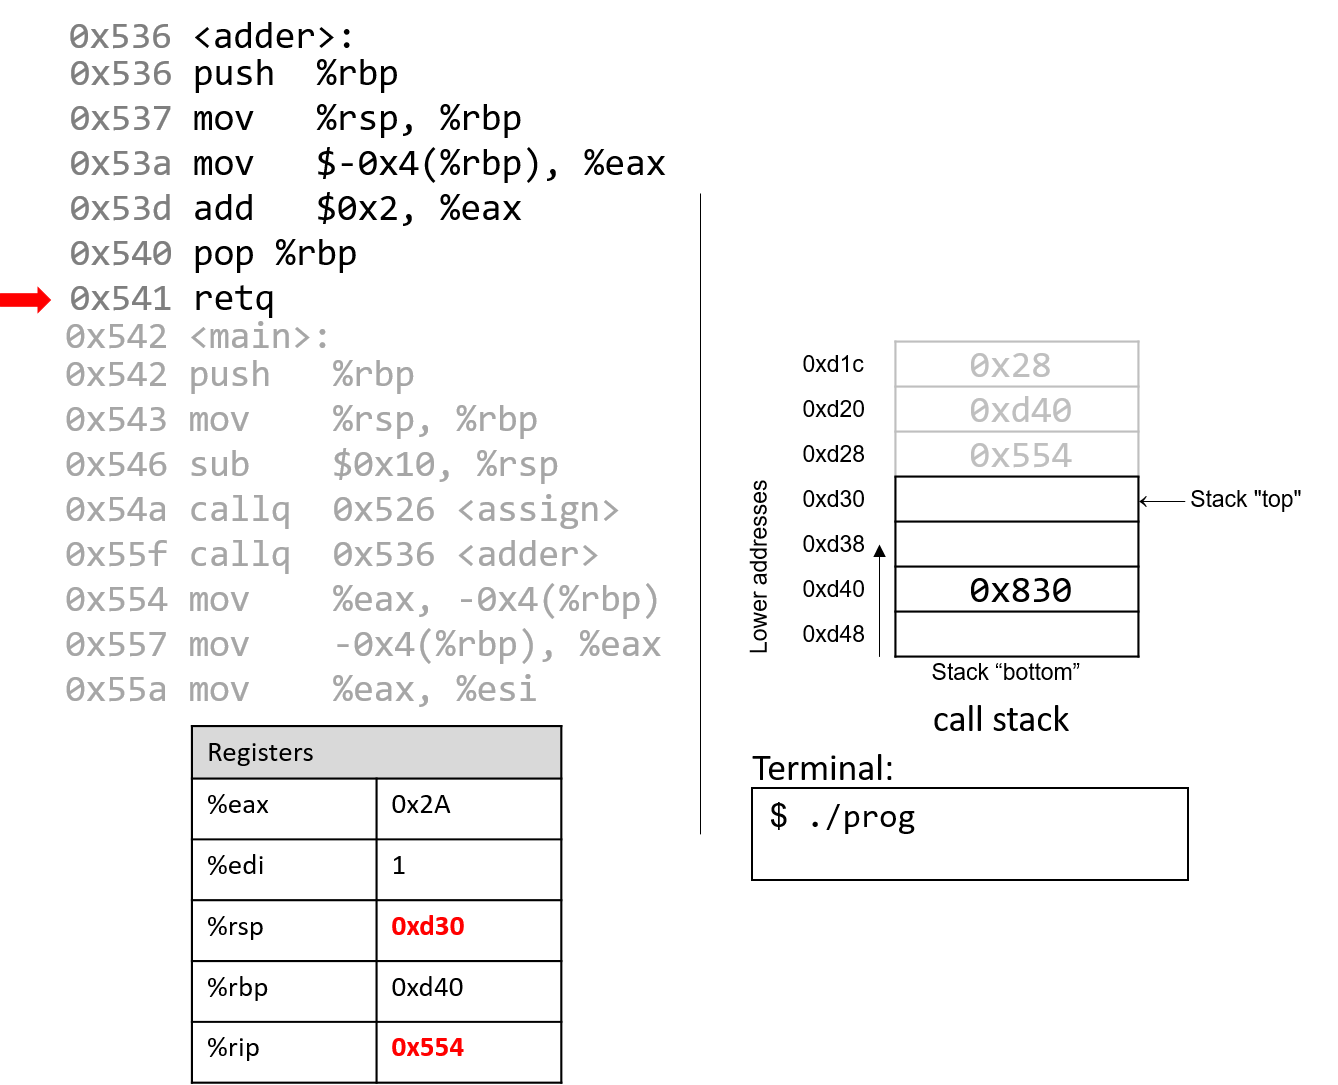
\includegraphics[scale=0.5]{img/Slide18.png}
        \end{center}

      \item Now it is relatively straightforward since we do the rest in main (except for the print statement). The current value in \texttt{\%eax} represents the return value of adder. We want to put this in the variable \texttt{x}, which we have already allocated some memory for right above the base pointer in the main stack frame. We move it there. Note that right after, it places this right back into \texttt{\%eax}.
        \begin{center}
          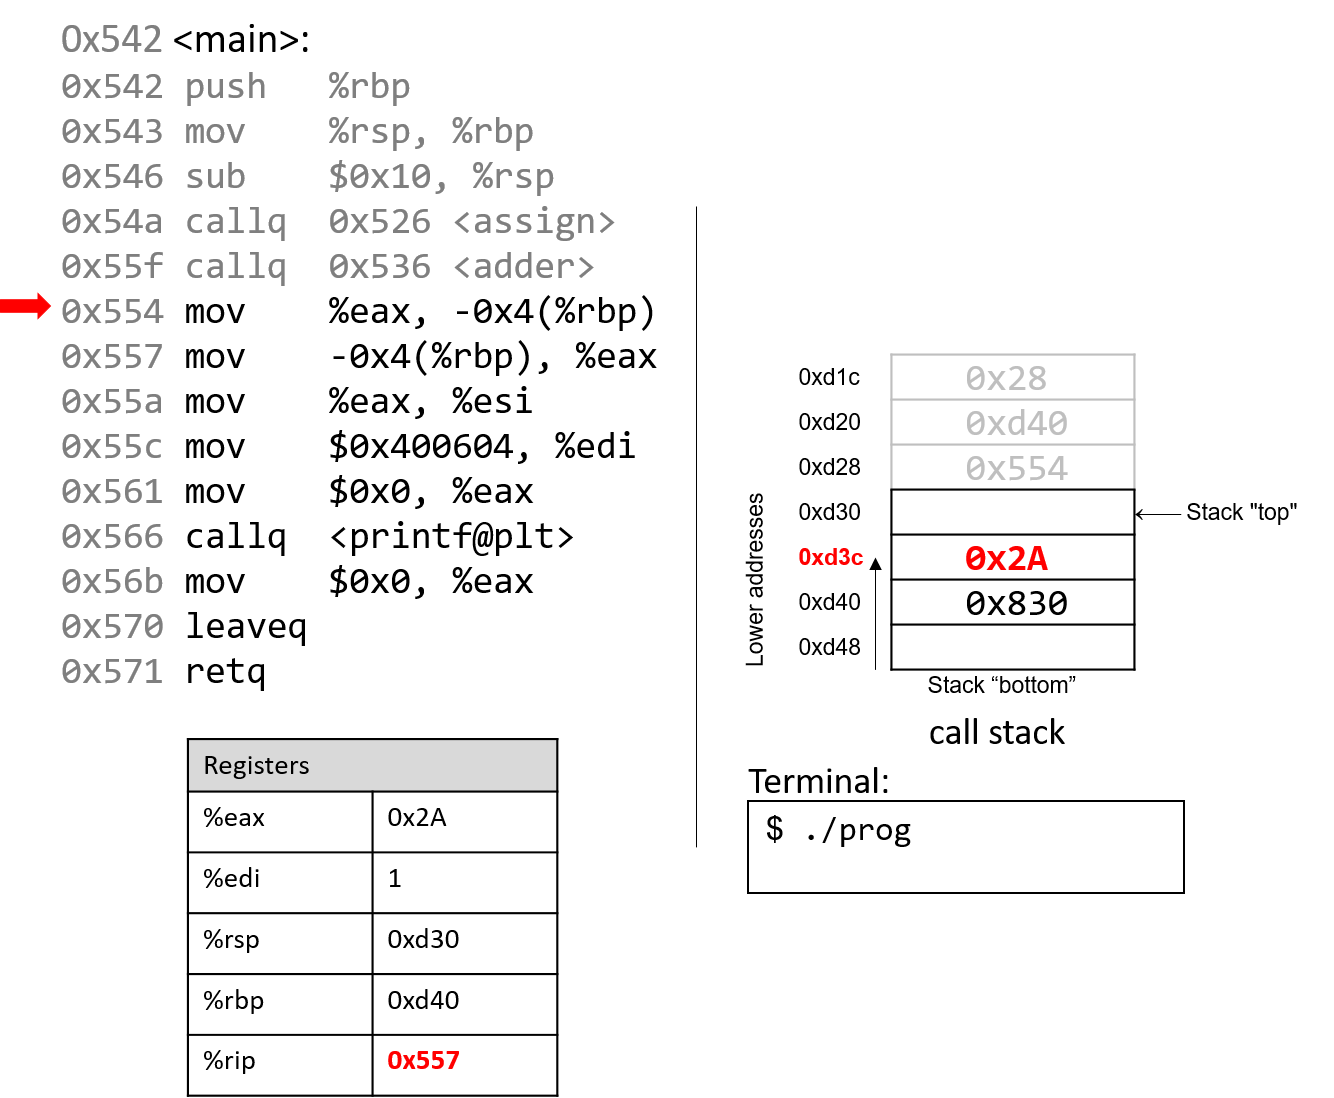
\includegraphics[scale=0.5]{img/Slide19.png}
        \end{center}

      \item the mov instruction at address 0x55a copies the value in \texttt{\%eax} (or 0x2A) to register \texttt{\%esi}, which is the 32-bit component register associated with \texttt{\%rsi} and typically stores the second parameter to a function. We can see why since this will be put into a print statement, which is a function, and \texttt{x = \%esi} is the second argument of \texttt{printf}. 
        \begin{center}
          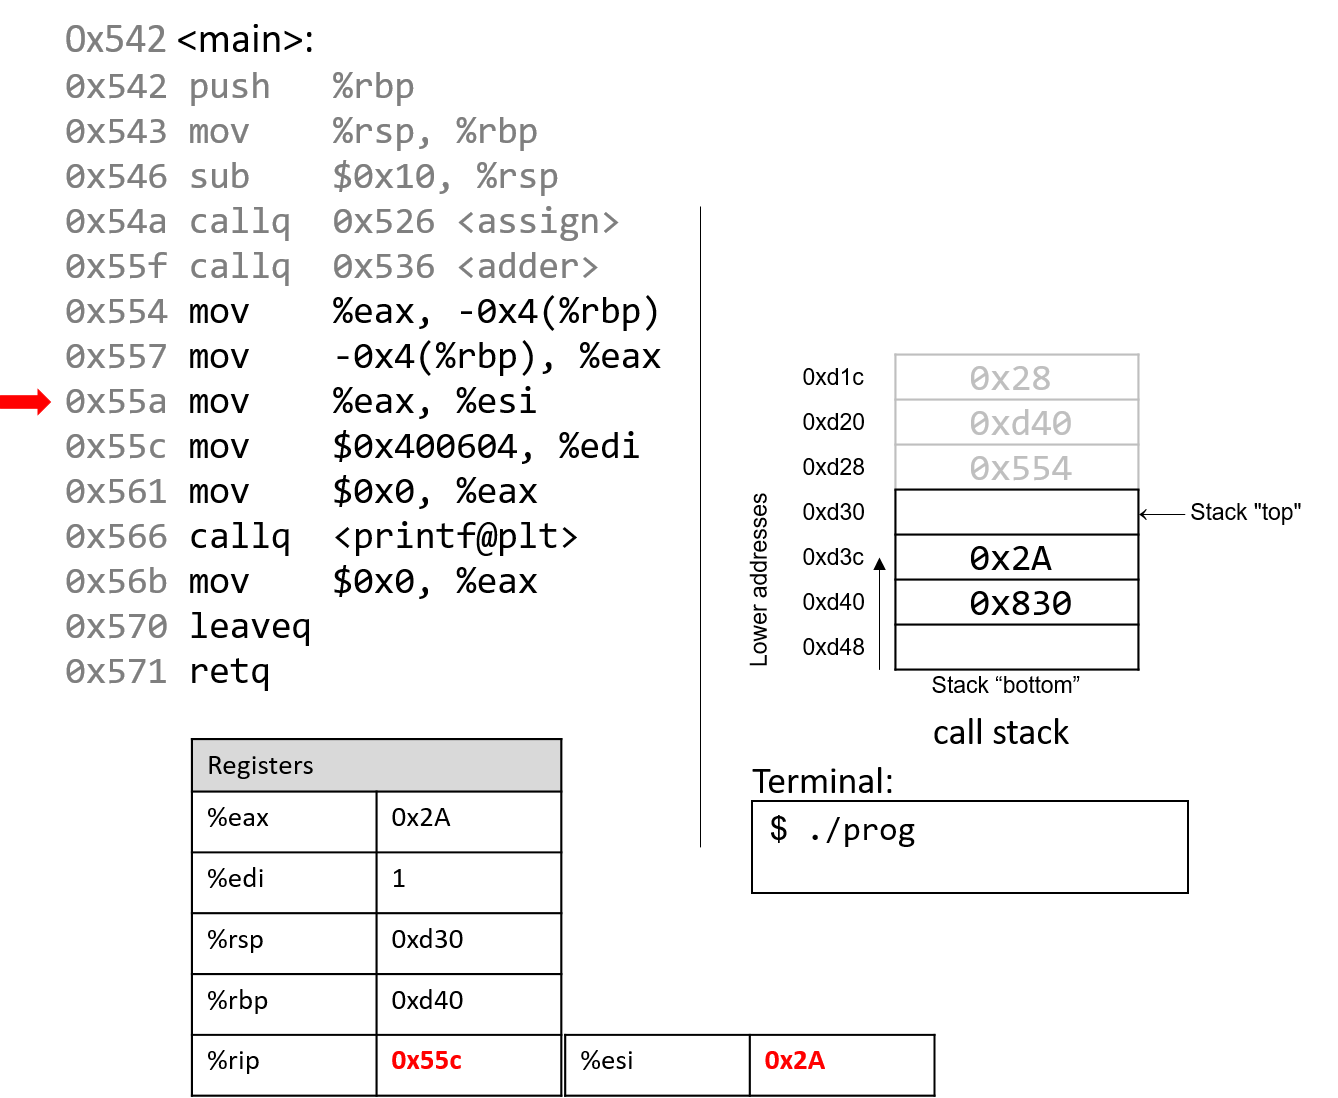
\includegraphics[scale=0.5]{img/Slide21.png}
        \end{center}

      \item Now we want to retrieve the first argument of the print function. The address at \texttt{\$0x400604} is some address in the code segment memory that holds the string \texttt{"x is \%d\textbackslash n"}. 
        \begin{center}
          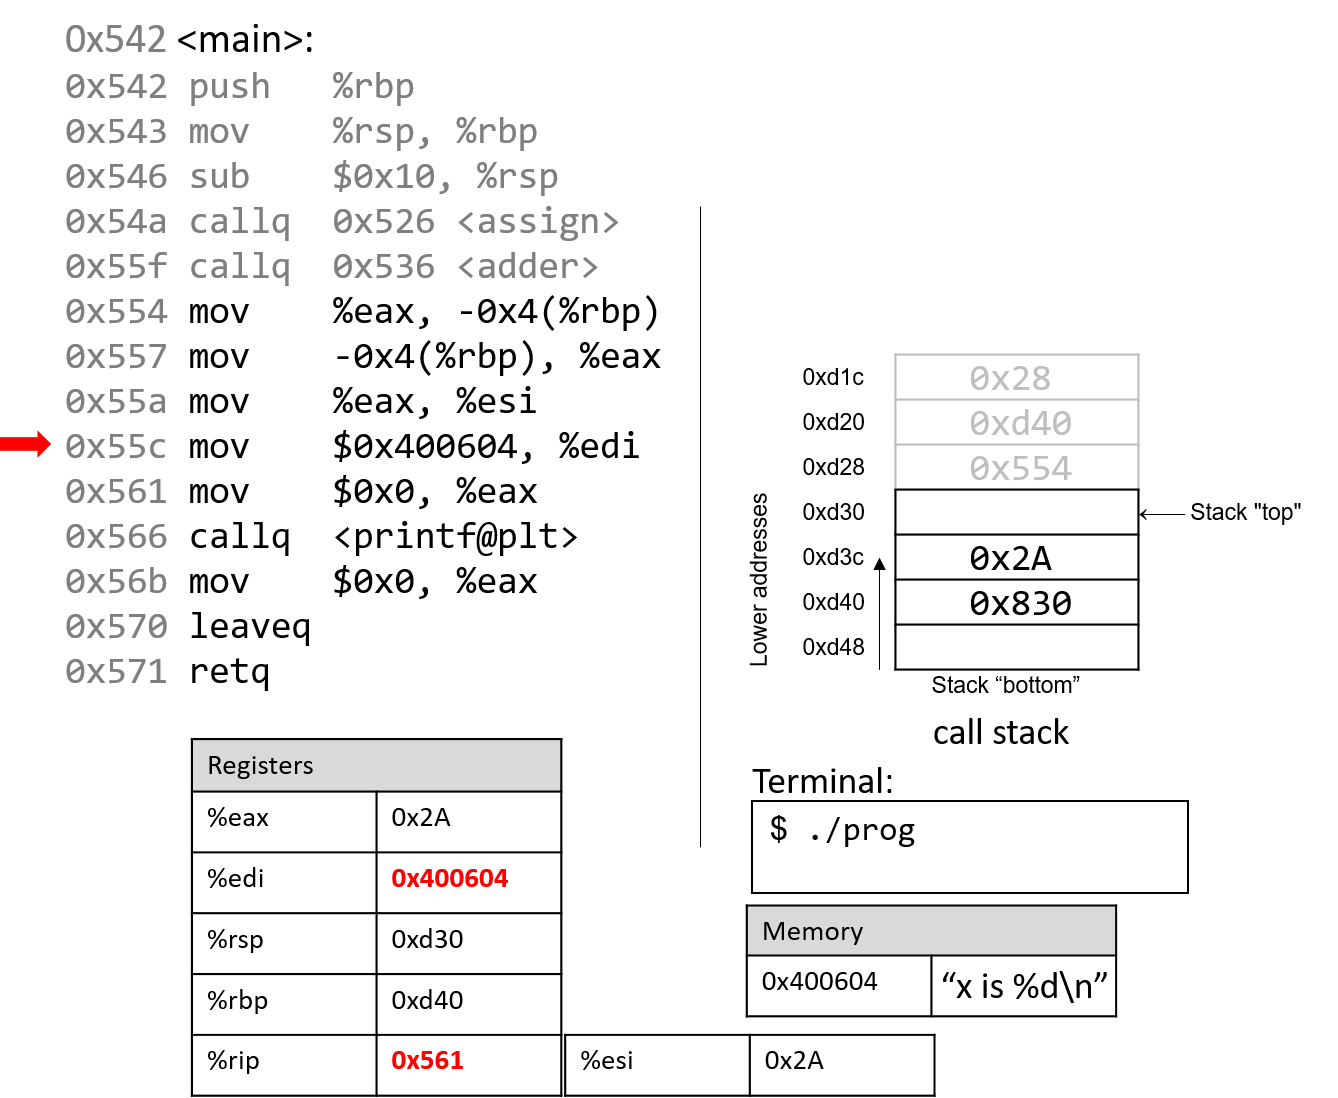
\includegraphics[scale=0.5]{img/Slide22.png}
        \end{center}

      \item Then we move $0$ into the \texttt{\%eax} register to clear it. 
        \begin{center}
          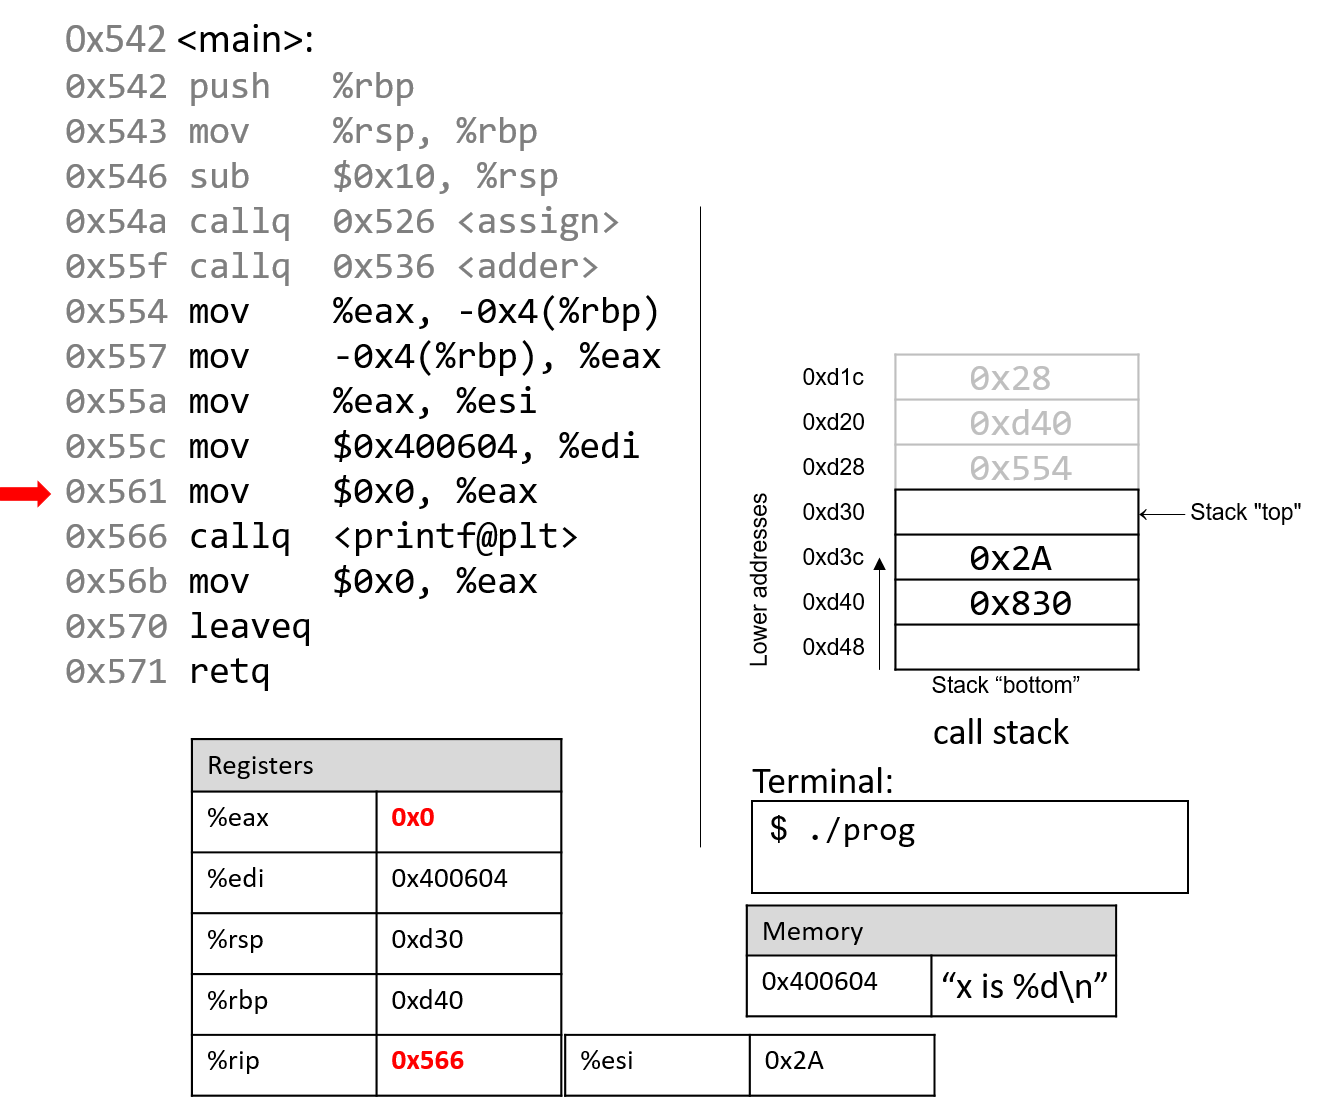
\includegraphics[scale=0.5]{img/Slide23.png}
        \end{center} 

      \item We then call the \texttt{printf} function, which we won't trace through but it outputs to stdout.  
        \begin{center}
          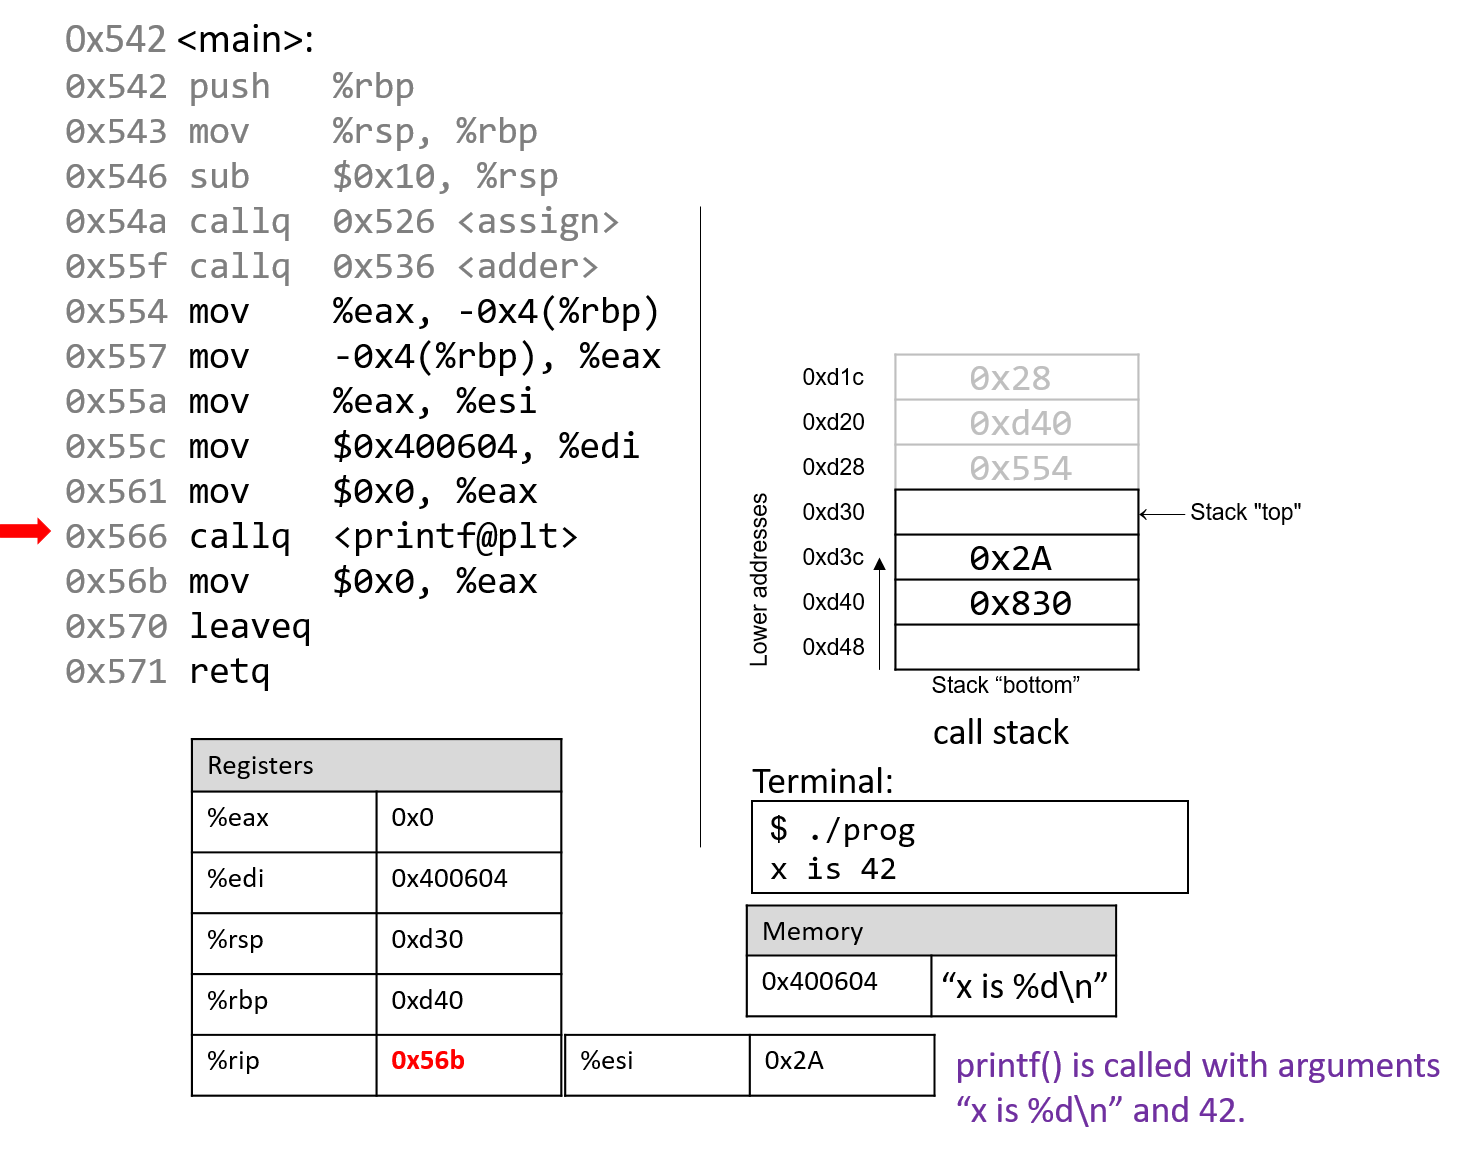
\includegraphics[scale=0.5]{img/Slide24.png}
        \end{center}

      \item The print function might have returned something, but we don't care. We want to main function to return 0, so we move 0 into \texttt{\%eax}. 
        \begin{center}
          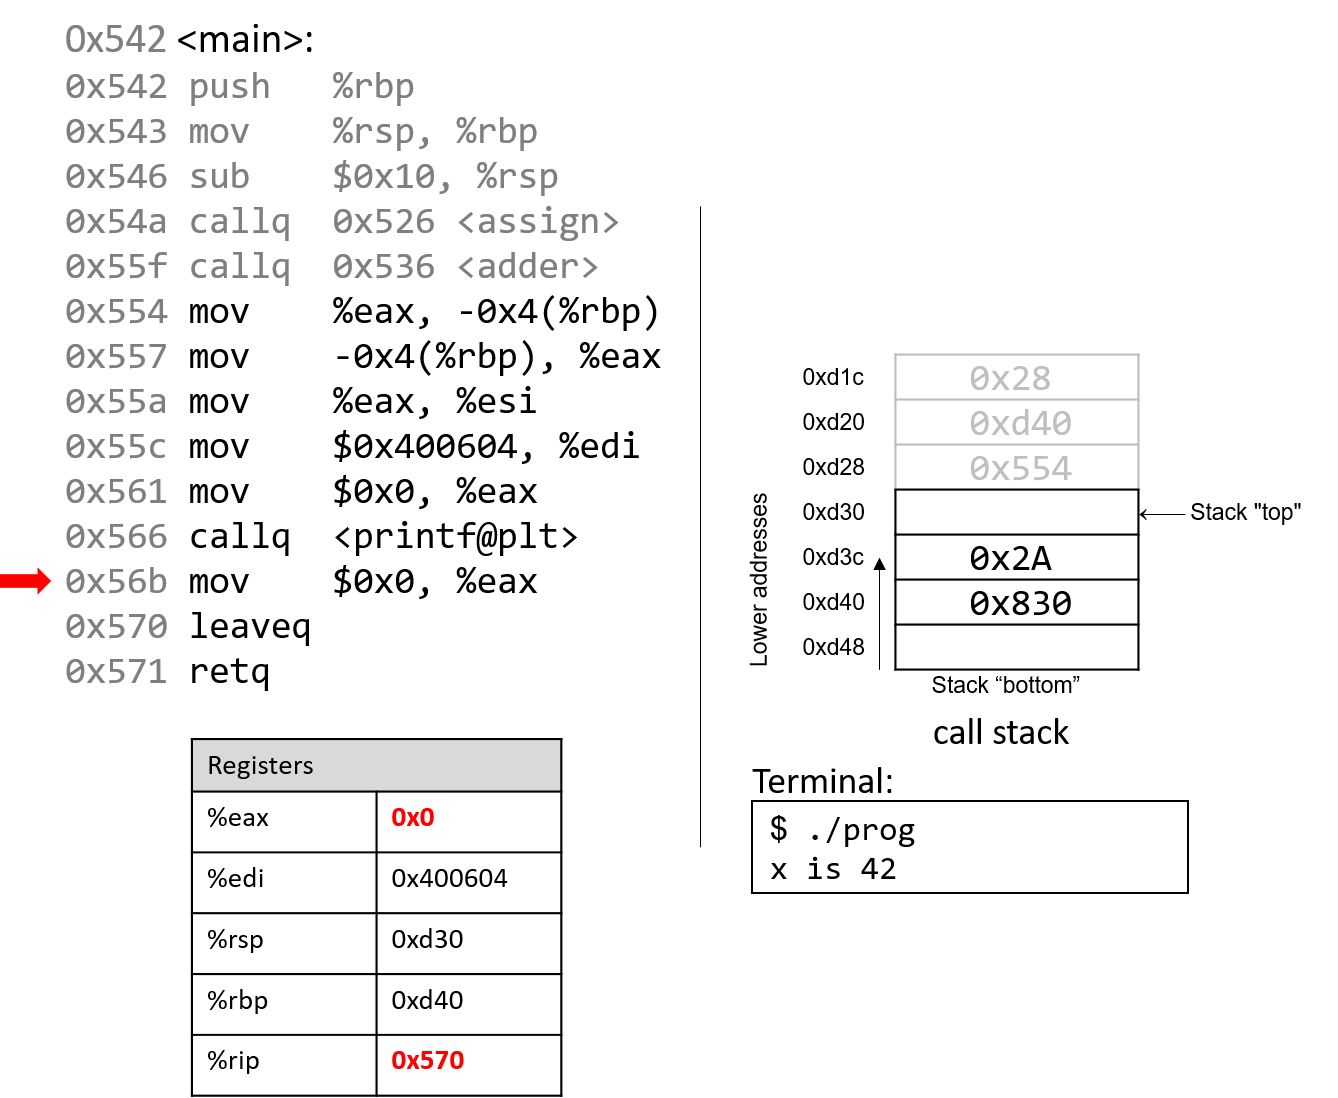
\includegraphics[scale=0.5]{img/Slide25.png}
        \end{center}

      \item Finally we execute \texttt{leaveq}, which prepares the stack for returning from the function call. It essentially moves the base pointer back to the stack pointer and then pops the base pointer off the stack. The new \texttt{\%rbp} is the original base pointer of whatever was outside the main function, \texttt{0x830}. 
        \begin{center}
          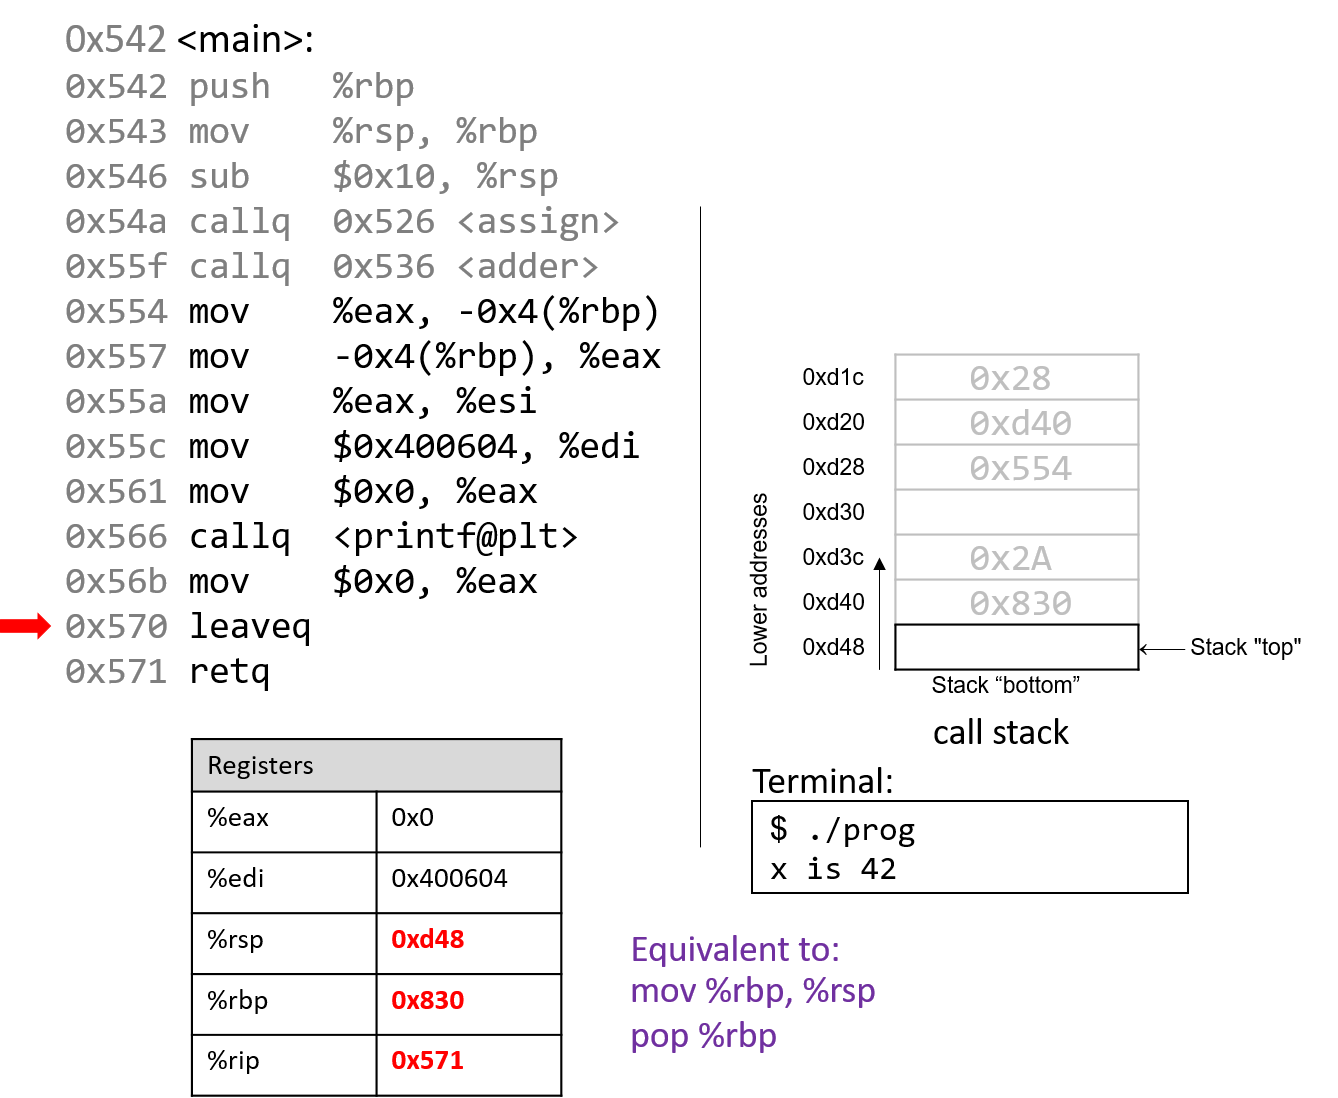
\includegraphics[scale=0.5]{img/Slide26.png}
        \end{center}

      \item Finally, we execute \texttt{retq}, which pops the return address off the stack and puts it into \texttt{\%rip}. 
    \end{enumerate}
  \end{example}

  We have omitted the details of caller and callee saved registers, but they do exist and are important for the general implementations. 

  For arrays, there's not anything new here. Let's go over some code and follow through it. 

  \begin{lstlisting}
    int sumArray(int *array, int length) {
      int i, total = 0;
      for (i = 0; i < length; i++) {
        total += array[i];
      }
      return total;
    }
  \end{lstlisting}

  This function takes the address of an array and the length of it and sums up all the elements in the array. 

  \begin{lstlisting}
    0x400686 <+0>:	push %rbp                   # save %rbp
    0x400687 <+1>:	mov  %rsp,%rbp              # update %rbp (new stack frame)
    0x40068a <+4>:	mov  %rdi,-0x18(%rbp)       # copy array to %rbp-0x18
    0x40068e <+8>:	mov  %esi,-0x1c(%rbp)       # copy length to %rbp-0x1c
    0x400691 <+11>:	movl $0x0,-0x4(%rbp)        # copy 0 to %rbp-0x4 (total)
    0x400698 <+18>:	movl $0x0,-0x8(%rbp)        # copy 0 to %rbp-0x8 (i)
    0x40069f <+25>:	jmp  0x4006be <sumArray+56> # goto <sumArray+56>
    0x4006a1 <+27>:	mov  -0x8(%rbp),%eax        # copy i to %eax
    0x4006a4 <+30>:	cltq                        # convert i to a 64-bit integer
    0x4006a6 <+32>:	lea  0x0(,%rax,4),%rdx      # copy i*4 to %rdx
    0x4006ae <+40>:	mov  -0x18(%rbp),%rax       # copy array to %rax
    0x4006b2 <+44>:	add  %rdx,%rax              # compute array+i*4, store in %rax
    0x4006b5 <+47>:	mov  (%rax),%eax            # copy array[i] to %eax
    0x4006b7 <+49>:	add  %eax,-0x4(%rbp)        # add %eax to total
    0x4006ba <+52>:	addl $0x1,-0x8(%rbp)        # add 1 to i (i+=1)
    0x4006be <+56>:	mov  -0x8(%rbp),%eax        # copy i to %eax
    0x4006c1 <+59>:	cmp  -0x1c(%rbp),%eax       # compare i to length
    0x4006c4 <+62>:	jl   0x4006a1 <sumArray+27> # if i<length goto <sumArray+27>
    0x4006c6 <+64>:	mov  -0x4(%rbp),%eax        # copy total to %eax
    0x4006c9 <+67>:	pop  %rbp                   # prepare to leave the function
    0x4006ca <+68>:	retq                        # return total
  \end{lstlisting}


\section{x86 Control Flow} 


\section{RISC-V Data Movement} 


\section{RISC-V Arithmetic Operations} 


\section{RISC-V Control Flow} 



\end{document}
